% Template:     Template Tesis LaTeX
% Documento:    Archivo principal
% Versión:      1.1.7 (02/10/2019)
% Codificación: UTF-8
%
% Autor: Pablo Pizarro R. @ppizarror
%        Facultad de Ciencias Físicas y Matemáticas
%        Universidad de Chile
%        pablo.pizarro@ing.uchile.cl, ppizarror.com
%
% Sitio web:    [https://latex.ppizarror.com/tesis]
% Licencia MIT: [https://opensource.org/licenses/MIT]
% CREACIÓN DEL DOCUMENTO
\documentclass[letterpaper,12pt,oneside]{book} % Libro, tamaño carta
\usepackage[utf8]{inputenc} % Codificación UTF-8
\bibliographystyle{unsrtnat}
% INFORMACIÓN DEL DOCUMENTO
\def\titulotesis {Modelamiento y seguimiento de tópicos para detección de modus operandi en robo de vehículos}
\def\titulogrado {
	Tesis para optar al grado de magíster en gestión de operaciones
	\bigbreak\vspace{0.3cm}
	Memoria para optar al título de ingeniero civil industrial
}

\def\nombreuniversidad {Universidad de Chile}
\def\nombrefacultad {Facultad de Ciencias Físicas y Matemáticas}
\def\departamentouniversidad {Departamento de Ingeniería Industrial}
\def\imagendepartamento {img/departamentos/uchile2.pdf}
\def\imagendepartamentoescala {0.7}
\def\localizacionuniversidad {Santiago, Chile}

% INTEGRANTES, PROFESORES Y FECHAS
\def\autortesis {DIEGO GARRIDO}
\def\fechatesis {\the\year}

\def\tablacomision {
\begin{tabular}{c}
	\vspace{1.5cm} \\
	\MakeUppercase{\textbf{\autortesis}} \\
	\vspace{1.0cm} \\
	PROFESOR GUÍA: \\
	RICHARD WEBER \\
	\vspace{0.5cm} \\
	MIEMBROS DE LA COMISIÓN: \\
	PROFESOR 2 \\
	PROFESOR 3 \\
	\vspace{0.5cm} \\
	Este trabajo ha sido parcialmente financiado por: \\
	NOMBRE INSTITUCIÓN \\
	\vspace{0.5cm} \\
	\MakeUppercase{\localizacionuniversidad} \\
	\MakeUppercase{\fechatesis}
\end{tabular}}{
}
\def\tablaresumen {
\begin{tabular}{l}
	RESUMEN DE LA MEMORIA PARA OPTAR \\
	AL TÍTULO DE MAGÍSTER EN CIENCIAS \\
	DE LA INGENIERÍA \\
	POR: \MakeUppercase{\textbf{\autortesis}} \\
	FECHA: \MakeUppercase{\fechatesis} \\
	PROF. GUÍA: RICHARD WEBER
\end{tabular}}{
}

% CONFIGURACIONES
% Template:     Presentación LaTeX
% Documento:    Configuraciones del template
% Versión:      1.4.5 (27/09/2021)
% Codificación: UTF-8
%
% Autor: Pablo Pizarro R.
%        pablo@ppizarror.com
%
% Manual template: [https://latex.ppizarror.com/presentacion]
% Licencia MIT:    [https://opensource.org/licenses/MIT]

% CONFIGURACIONES GENERALES
\def\compilertype {pdf2latex}      % Compilador {pdf2latex,xelatex,lualatex}
\def\documentfontsize {10}         % Tamaño de la fuente del documento [pt]
\def\documentinterline {1}         % Interlineado del documento [factor]
\def\documentparindent {0}         % Tamaño del indentado de párrafos [pt]
\def\documentparskip {0}           % Tamaño adicional entre párrafos (+/-) [pt]
\def\fontdocument {lmodern}        % Tipografía base, ver soportadas en manual
\def\fonttypewriter {tmodern}      % Tipografía de \texttt, ver manual
\def\fonturl {same}                % Tipo de fuente url {tt,sf,rm,same}
\def\frametextjustified {true}     % Justifica todos los párrafos de los frames
\def\graphicxdraft {false}         % En true no carga las imágenes (modo draft)
\def\pointdecimal {true}           % N° decimales con punto en vez de coma
\def\showlayoutlines {false}       % Muestra el layout de la página

% CONFIGURACIÓN DE LAS LEYENDAS - CAPTION
\def\captionalignment {justified}  % Posición {centered,justified,left,right}
\def\captionfontsize{footnotesize} % Tamaño de fuente de los caption
\def\captionlabelformat {simple}   % Formato leyenda {empty,simple,parens}
\def\captionlabelsep {colon}       % Sep. {none,colon,period,space,quad,newline}
\def\captionlessmarginimage {0.1}  % Margen sup/inf de figura sin leyenda [cm]
\def\captionlrmargin {0}           % Márgenes izq/der de la leyenda [cm]
\def\captionlrmarginmc {0}         % Margen izq/der leyenda dentro de cols. [cm]
\def\captionmarginimage {0}        % Margen vertical entre caption e imagen [cm]
\def\captionmarginimages {-0.04}   % Margen vertical entre caption e images [cm]
\def\captionmarginimagesmc {-0.04} % Margen vert. entre caption e imagesmc [cm]
\def\captionmarginmultimg {0}      % Margen izq/der leyendas múltiple img [cm]
\def\captionnumcode {arabic}       % N° código {arabic,alph,Alph,roman,Roman}
\def\captionnumequation {arabic}   % N° ecuac. {arabic,alph,Alph,roman,Roman}
\def\captionnumfigure {arabic}     % N° figuras {arabic,alph,Alph,roman,Roman}
\def\captionnumsubfigure {alph}    % N° subfigs. {arabic,alph,Alph,roman,Roman}
\def\captionnumsubtable {alph}     % N° subtabla {arabic,alph,Alph,roman,Roman}
\def\captionnumtable {arabic}      % N° tabla {arabic,alph,Alph,roman,Roman}
\def\captionsubchar {.}            % Caracter entre N° objeto - subfigura/tabla
\def\captiontbmarginfigure {9.35}  % Margen sup/inf de leyenda en figuras [pt]
\def\captiontbmargintable {7}      % Margen sup/inf de la leyenda en tablas [pt]
\def\captiontextbold {true}        % Etiqueta (código,figura,tabla) en negrita
\def\captiontextsubnumbold {true}  % N° subfigura/subtabla en negrita
\def\codecaptiontop {true}         % Leyenda arriba del código fuente
\def\equationcaptioncenter {true}  % Ecuaciones están centradas o justificadas
\def\figurecaptiontop {false}      % Leyenda arriba de las imágenes
\def\marginaligncaptbottom {0.1}   % Margen inferior caption en align [cm]
\def\marginaligncapttop {-0.75}    % Margen superior caption en align [cm]
\def\marginalignedcaptbottom {0.1} % Margen inferior caption en aligned [cm]
\def\marginalignedcapttop {-0.75}  % Margen superior caption en aligned [cm]
\def\margineqncaptionbottom {0}    % Margen inferior caption ecuación [cm]
\def\margineqncaptiontop {-0.7}    % Margen superior caption ecuación [cm]
\def\margingathercaptbottom {0.1}  % Margen inferior caption en gather [cm]
\def\margingathercapttop {-0.9}    % Margen superior caption en gather [cm]
\def\margingatheredcaptbottom{0.1} % Margen inferior caption en gathered [cm]
\def\margingatheredcapttop {-0.7}  % Margen superior caption en gathered [cm]
\def\sectioncaptiondelimiter {.}   % Caracter delimitador n° objeto y sección
\def\showsectioncaptioncode {none} % N° sec código {none,chap,(s/ss/sss/ssss)ec}
\def\showsectioncaptioneqn {none}  % N° sec ecuac. {none,chap,(s/ss/sss/ssss)ec}
\def\showsectioncaptionfig {none}  % N° sec figs. {none,chap,(s/ss/sss/ssss)ec}
\def\showsectioncaptionmat {none}  % N° matemático {none,chap,(s/ss/sss/ssss)ec}
\def\showsectioncaptiontab {none}  % N° sec tablas {none,chap,(s/ss/sss/ssss)ec}
\def\subcaptionfsize{footnotesize} % Tamaño de la fuente de los subcaption
\def\subcaptionlabelformat{parens} % Formato leyenda sub. {empty,simple,parens}
\def\subcaptionlabelsep {space}    % Sep. {none,colon,period,space,quad,newline}
\def\tablecaptiontop {true}        % Leyenda arriba de las tablas

% ANEXO, CITAS, REFERENCIAS
\def\bibtexrefsep {5}              % Separación entre refs. {bibtex} [pt]
\def\bibtexstyle {apalike}         % Formato refs. bibtex {apa,ieeetr,etc...}
\def\stylecitereferences {bibtex}  % Estilo cita/ref {bibtex,custom}

% CONFIGURACIONES DE OBJETOS
\def\columnsepwidth {2.1}          % Separación entre columnas [em]
\def\defaultimagefolder {img/}     % Carpeta raíz de las imágenes
\def\equationleftalign {false}     % Ecuaciones alineadas a la izquierda
\def\equationrestart {none}        % Reinicio n° {none,chap,(s/ss/sss/ssss)ec}
\def\footnotelmargin {10}          % Margen entre footnote y el número [pt]
\def\footnoterestart {none}        % N° foot. {none,chap,page,(s/ss/sss/ssss)ec}
\def\footnoterulefigure {false}    % Footnote en figuras tienen línea superior
\def\footnoterulepage {false}      % Footnote en páginas tienen línea superior
\def\footnoteruletable {false}     % Footnote en tablas tienen línea superior
\def\footnotetwocolumn {false}     % Footnote en dos columnas
\def\fpremovetopbottomcenter{true} % Elimina espacio vert. al centrar con b!,t!
\def\imagedefaultplacement {H}     % Posición por defecto de las imágenes
\def\marginalignbottom {-0.4}      % Margen inferior entorno align [cm]
\def\marginalignedbottom {-0.2}    % Margen inferior entorno aligned [cm]
\def\marginalignedtop {-0.4}       % Margen superior entorno aligned [cm]
\def\marginaligntop {-0.4}         % Margen superior entorno align [cm]
\def\marginequationbottom {-0.2}   % Margen inferior ecuaciones [cm]
\def\marginequationtop {0}         % Margen superior ecuaciones [cm]
\def\marginfloatimages {-13}       % Margen sup figs. insertimageleft/right [pt]
\def\margingatherbottom {-0.2}     % Margen inferior entorno gather [cm]
\def\margingatheredbottom {-0.1}   % Margen inferior entorno gathered [cm]
\def\margingatheredtop {-0.4}      % Margen superior entorno gathered [cm]
\def\margingathertop {-0.4}        % Margen superior entorno gather [cm]
\def\marginimagebottom {-0.50}     % Margen inferior figura [cm]
\def\marginimagemultbottom {-0.05} % Margen inferior imágenes múltiples [cm]
\def\marginimagemultright {0.35}   % Margen derecho imágenes múltiples [cm]
\def\marginimagemulttop {-0.3}     % Margen superior imágenes múltiples [cm]
\def\marginimagetop {0}            % Margen superior figuras [cm]
\def\numberedequation {true}       % Ecuaciones con \insert... numeradas
\def\senumerti {\arabic{enumi}.}   % Estilo enumerate nivel 1
\def\senumertii {\alph{enumii})}   % Estilo enumerate nivel 2
\def\senumertiii{\roman{enumiii}.} % Estilo enumerate nivel 3
\def\senumertiv {\Alph{enumiv})}   % Estilo enumerate nivel 4
\def\sitemizei {\iitembcirc}       % Estilo itemize nivel 1
\def\sitemizeii {\iitemdash}       % Estilo itemize nivel 2
\def\sitemizeiii {\iitemcirc}      % Estilo itemize nivel 3
\def\sitemizeiv {\iitembsquare}    % Estilo itemize nivel 4
\def\sourcecodebtmargin {0}        % Margen superior e inferior del bloque [pt]
\def\sourcecodefontf {\ttfamily}   % Tipo de letra código fuente
\def\sourcecodefonts{\footnotesize}% Tamaño letra código fuente
\def\sourcecodeilfontf {\ttfamily} % Tipo de letra código fuente inline
\def\sourcecodeilfonts {\small}    % Tamaño letra código fuente inline
\def\sourcecodenumbersep {3}       % Separación entre número línea y código [pt]
\def\sourcecodenumbersize {\tiny}  % Tamaño fuente número línea
\def\sourcecodeskipabove {0.75}    % Espacio sobre recuadro código [em]
\def\sourcecodeskipbelow {1}       % Espacio bajo recuadro código [em]
\def\sourcecodetabsize {3}         % Tamaño tabulación código fuente
\def\tabledefaultplacement {H}     % Posición por defecto de las tablas
\def\tablenotesameline {true}      % Notas en tablas en una sola línea
\def\tablenotesfontsize {\small}   % Tamaño de fuente de las notas en tablas
\def\tablepaddingh {0.75}          % Espaciado horizontal de celda de las tablas
\def\tablepaddingv {1.15}          % Espaciado vertical de celda de las tablas
\def\tikzdefaultplacement {H}      % Posición por defecto de las figuras tikz

% CONFIGURACIÓN DE LOS COLORES DEL DOCUMENTO
\def\captioncolor {black}          % Color nombre objeto (código,figura,tabla)
\def\captiontextcolor {black}      % Color de la leyenda
\def\highlightcolor {yellow}       % Color del subrayado con \hl
\def\linenumbercolor {gray}        % Color del n° de línea (\showlinenumbers)
\def\linkcolor {black}             % Color de los links del documento
\def\maintextcolor {black}         % Color principal del texto
\def\numcitecolor {black}          % Color del n° de las referencias o citas
\def\pagescolor {white}            % Color de la página
\def\showborderonlinks {false}     % Color de un link por un recuadro de color
\def\sourcecodebgcolor {lgray}     % Color de fondo del código fuente
\def\tablelinecolor {black}        % Color de las líneas de las tablas
\def\tablerowfirstcolor {none}     % Primer color de celda de las tablas
\def\tablerowsecondcolor {gray!20} % Segundo color de celda de las tablas
\def\urlcolor {magenta}            % Color de los enlaces web (\href,\url)

% OPCIONES DEL PDF COMPILADO
\def\cfgbookmarksopenlevel {1}     % Nivel marcadores en pdf (1:secciones)
\def\cfgpdfbookmarkopen {true}     % Expande marcadores del nivel configurado
\def\cfgpdfcenterwindow {true}     % Centra ventana del lector al abrir el pdf
\def\cfgpdfcopyright {}            % Establece el copyright del documento
\def\cfgpdfdisplaydoctitle {true}  % Muestra título del informe en visor
\def\cfgpdffitwindow {true}        % Ajusta la ventana del lector tamaño pdf
\def\cfgpdfkeywords {}             % Palabras clave del pdf
\def\cfgpdflayout {OneColumn}      % Modo de página {OneColumn,SinglePage}
\def\cfgpdfmenubar {true}          % Muestra el menú del lector
\def\cfgpdfpageview {FitBV}        % {Fit,FitH,FitV,FitR,FitB,FitBH,FitBV}
\def\cfgpdfsecnumbookmarks {true}  % Número de la sec. en marcadores del pdf
\def\cfgpdftoolbar {true}          % Muestra barra de herramientas lector pdf
\def\cfgshowbookmarkmenu {false}   % Muestra menú marcadores al abrir el pdf
\def\indexdepth {4}                % Profundidad de los marcadores
\def\pdfcompilecompression {9}     % Factor de compresión del pdf (0-9)
\def\pdfcompileobjcompression {2}  % Nivel compresión objetos del pdf (0-3)
\def\usepdfmetadata {true}         % Añade metadatos al pdf compilado

% NOMBRE DE OBJETOS
\def\nameltappendixsection {Anexo} % Etiqueta sección en anexo/apéndices
\def\nameltwfigure {Figura}        % Etiqueta leyenda de las figuras
\def\nameltwsrc {Código}           % Etiqueta leyenda del código fuente
\def\nameltwtable {Tabla}          % Etiqueta leyenda de las tablas
\def\namemathcol {Corolario}       % Nombre de los colorarios
\def\namemathdefn {Definición}     % Nombre de las definiciones
\def\namemathej {Ejemplo}          % Nombre de los ejemplos
\def\namemathlem {Lema}            % Nombre de los lemas
\def\namemathobs {Observación}     % Nombre de las observaciones
\def\namemathprp {Proposición}     % Nombre de las proposiciones
\def\namemaththeorem {Teorema}     % Nombre de los teoremas
\def\namereferences {Referencias}  % Nombre de la sección de referencias

% CONFIGURA BEAMER
% https://latex.ppizarror.com/doc/beameruserguide.pdf
\mode<presentation> {
	
	% LISTA DE TEMAS GLOBALES, DESCONFIGURAR PARA APLICAR
	% https://latex.ppizarror.com/beamer_themes.html
	
	% \usetheme{AnnArbor}
	% \usetheme{Antibes}
	% \usetheme{Bergen}
	% \usetheme{Berkeley}
	% \usetheme{Berlin}
	% \usetheme{Boadilla}
	% \usetheme{boxes}
	% \usetheme{CambridgeUS}
	% \usetheme{Copenhagen}
	% \usetheme{Darmstadt}
	% \usetheme{default}
	% \usetheme{Dresden}
	% \usetheme{Frankfurt}
	% \usetheme{Goettingen}
	% \usetheme{Hannover}
	% \usetheme{Ilmenau}
	% \usetheme{JuanLesPins}
	% \usetheme{Luebeck}
	\usetheme{Madrid}
	% \usetheme{Malmoe}
	% \usetheme{Marburg}
	% \usetheme{Montpellier}
	% \usetheme{PaloAlto}
	% \usetheme{Pittsburgh}
	% \usetheme{Rochester}
	% \usetheme{Singapore}
	% \usetheme{Szeged}
	% \usetheme{Warsaw}
	
	% TEMAS TIPO <INNER>, USAR SÓLO SI NO SE APLICA EL GLOBAL
	% https://latex.ppizarror.com/doc/Beamer-appearance-cheat-sheet.pdf
	
	% \useinnertheme{default}
	% \useinnertheme{circles}
	%\useinnertheme{rectangles}
	% \useinnertheme{rounded}
	% \useinnertheme{inmargin}
	
	% TEMAS TIPO <OUTER>, USAR SÓLO SI NO SE APLICA EL GLOBAL
	
	% \useoutertheme{default}
	%\useoutertheme{infolines}
	% \useoutertheme{miniframes}
	% \useoutertheme{smoothbars}
	% \useoutertheme{sidebar}
	% \useoutertheme{split}
	% \useoutertheme{shadow}
	% \useoutertheme{tree}
	% \useoutertheme{smoothtree}
	
	% COLORES DE LA SLIDE, USAR SÓLO SI NO SE APLICA EL GLOBAL
	% https://latex.ppizarror.com/beamer_colors.html
	
	% \usecolortheme{default}
	%\usecolortheme[named=cardinalred]{structure}
	% \usecolortheme{sidebartab}
	
	% \usecolortheme{albatross}
	% \usecolortheme{beaver}
	% \usecolortheme{beetle}
	% \usecolortheme{crane}
	% \usecolortheme{dolphin}
	% \usecolortheme{dove}
	% \usecolortheme{fly}
	% \usecolortheme{lily}
	% \usecolortheme{monarca}
	%\usecolortheme{orchid}
	% \usecolortheme{rose}
	% \usecolortheme{seagull}
	% \usecolortheme{seahorse}
	% \usecolortheme{spruce}
	%\usecolortheme{whale}
	% \usecolortheme{wolverine}
	
	% CONFIGURACIONES GENERALES
	\def\itemizedeleteleftmargin {true}
	\def\tabularframeopacity {0.4}
	\def\tabularframepaddingleft {0.2}
	\def\tabularframepaddingright {0.2}
	\def\tabularframepaddingtop {0.15}
	
	% CONFIGURA LOS BLOQUES, VALORES EN [EM]
	\def\blockmarginbottom {1}
	\def\blockpaddingbottom {0.6}
	\def\blockpaddingleft {0.6}
	\def\blockpaddingright {0.6}
	\def\blockpaddingtop {0.75}
	
	% PARA RESTABLECER EL HEADLINE, COMENTAR
	\setbeamertemplate{headline}{}
	
	% ELEMENTOS CON \pause o \onslide ESTÁN OCULTOS
	\setbeamercovered{invisible}
	% \setbeamercovered{transparent}
	
	% PARA ELIMINAR EL FOOTER, DESCOMENTAR
	% \setbeamertemplate{footline}{}
	
	% REEMPLAZAR EL FOOTER POR EL N° DE PÁGINA
	% \setbeamertemplate{footline}[page number]
	
	% PARA ACTIVAR LOS SÍMBOLOS DE NAVEGACIÓN, COMENTAR
	\setbeamertemplate{navigation symbols}{}
	
}


% IMPORTACIÓN DE LIBRERÍAS
% Template:     Template Tesis LaTeX
% Documento:    Importación de librerías
% Versión:      1.1.7 (02/10/2019)
% Codificación: UTF-8
%
% Autor: Pablo Pizarro R.
%        Facultad de Ciencias Físicas y Matemáticas
%        Universidad de Chile
%        pablo@ppizarror.com
%
% Sitio web:    [https://latex.ppizarror.com/tesis]
% Licencia MIT: [https://opensource.org/licenses/MIT]

\usepackage[spanish,es-nosectiondot,es-lcroman,es-noquoting]{babel}
\usepackage{ifthen}
\newcommand{\throwbadconfig}[4][]{
	\ifthenelse{\equal{#1}{noheader}}{
		\errmessage{LaTeX Warning: #4}
	}{
		\ifthenelse{\equal{#1}{noheader-nostop}}{
			\errmessage{LaTeX Warning: #4}
		}{
			\errmessage{LaTeX Warning: #2 \noexpand #3=#3. Valores esperados: #4}
		}
	}
	\ifthenelse{\equal{#1}{nostop}}{}{
		\ifthenelse{\equal{#1}{noheader-nostop}}{}{
			\stop
		}
	}
}
\ifthenelse{\equal{\equationleftalign}{true}}{
	\usepackage[fleqn]{amsmath}
}{
	\usepackage{amsmath}
}
\let\counterwithout\relax
\let\counterwithin\relax
\let\RE\Re
\let\IM\Im
\usepackage{amssymb}
\usepackage{amsthm}
\usepackage{array}
\usepackage{bigstrut}
\usepackage{bm}
\usepackage{booktabs}
\usepackage{caption}
\usepackage{changepage}
\usepackage{chngcntr}
\usepackage{color}
\usepackage{datetime}
\usepackage{floatpag}
\usepackage{floatrow}
\usepackage{framed}
\usepackage{gensymb}
\usepackage{geometry}
\usepackage{graphicx}
\usepackage{lipsum}
\usepackage{listings}
\usepackage{listingsutf8}
\usepackage{longtable}
\usepackage{mathtools}
\usepackage{multicol}
\usepackage{needspace}
\usepackage{pdflscape}
\usepackage{pdfpages}
\usepackage{physics}
\usepackage{rotating}
\usepackage{sectsty}
\usepackage{selinput}
\usepackage{setspace}
\usepackage{soul}
\usepackage{subfig}
\usepackage{textcomp}
\usepackage{url}
\usepackage{wasysym}
\usepackage{wrapfig}
\usepackage{xspace}
\usepackage[makeroom]{cancel}
\usepackage[inline]{enumitem}
\usepackage[subfigure,titles]{tocloft}
\usepackage[figure,table,lstlisting]{totalcount}
\usepackage[normalem]{ulem}
\usepackage[dvipsnames,table,usenames]{xcolor}
\ifthenelse{\equal{\footnotepagetoprule}{true}}{
\usepackage[bottom,hang]{footmisc}
}{
	\usepackage[bottom,norule,hang]{footmisc}
}
\ifthenelse{\equal{\showdotaftersnum}{true}}{
	\usepackage{secdot}
	\sectiondot{subsection}
	\sectiondot{subsubsection}}{
}
\usepackage[pdfencoding=auto,psdextra]{hyperref}
\ifthenelse{\equal{\stylecitereferences}{natbib}}{
	\ifthenelse{\equal{\natbibrefstyle}{apa}}{
		\ifthenelse{\equal{\natbibsquare}{true}}{
			\usepackage[square]{natbib}
		}{
			\usepackage[round]{natbib}
		}
	}{
	\ifthenelse{\equal{\natbibrefstyle}{ieeetr}}{
		\ifthenelse{\equal{\natbibsquare}{true}}{
			\usepackage[square,numbers]{natbib}
		}{
			\usepackage[round,numbers]{natbib}
		}
	}{
	\ifthenelse{\equal{\natbibrefstyle}{unsrt}}{
		\ifthenelse{\equal{\natbibsquare}{true}}{
			\usepackage[square,numbers]{natbib}
		}{
			\usepackage[round,numbers]{natbib}
		}
	}{
	\ifthenelse{\equal{\natbibrefstyle}{abbrvnat}}{
		\ifthenelse{\equal{\natbibsquare}{true}}{
			\usepackage[square,numbers]{natbib}
		}{
			\usepackage[round,numbers]{natbib}
		}
	}{
		\ifthenelse{\equal{\natbibnumbers}{true}}{
			\ifthenelse{\equal{\natbibsquare}{true}}{
				\usepackage[square,numbers]{natbib}
			}{
				\usepackage[round,numbers]{natbib}
			}
		}{
			\ifthenelse{\equal{\natbibsquare}{true}}{
				\usepackage[square]{natbib}
			}{
				\usepackage[round]{natbib}
			}
		}
	}}}}
	\usepackage[nottoc,notlof,notlot]{tocbibind}
}{
\ifthenelse{\equal{\stylecitereferences}{apacite}}{
		\usepackage{apacite}
		\usepackage[nottoc,notlof,notlot]{tocbibind}
	}{
\ifthenelse{\equal{\stylecitereferences}{bibtex}}{
		}{}
	}
}
\ifthenelse{\equal{\showappendixsecindex}{true}}{
	\usepackage[toc]{appendix}
}{
	\usepackage{appendix}
}
\ifthenelse{\equal{\importtikz}{true}}{
	\usepackage{tikz}}{
}
\usepackage{bookmark}
\usepackage{fancyhdr}
\usepackage{float}
\usepackage{hyperxmp}
\usepackage{multirow}
\usepackage{notoccite}
\usepackage{titlesec}
\ifthenelse{\equal{\fontdocument}{lmodern}}{
	\usepackage{lmodern}
}{
\ifthenelse{\equal{\fontdocument}{arial}}{
	\usepackage{helvet}
	\renewcommand{\familydefault}{\sfdefault}
}{
\ifthenelse{\equal{\fontdocument}{arial2}}{
	\usepackage{arial}
}{
\ifthenelse{\equal{\fontdocument}{times}}{
	\usepackage{mathptmx}
}{
\ifthenelse{\equal{\fontdocument}{helvet}}{
	\usepackage{helvet}
}{
\ifthenelse{\equal{\fontdocument}{alegreyasans}}{
	\usepackage[sfdefault]{AlegreyaSans}
	\renewcommand*\oldstylenums[1]{{\AlegreyaSansOsF #1}}
}{
\ifthenelse{\equal{\fontdocument}{mathpazo}}{
	\usepackage{mathpazo}
}{
\ifthenelse{\equal{\fontdocument}{accantis}}{
	\usepackage{accanthis}
}{
\ifthenelse{\equal{\fontdocument}{alegreya}}{
	\usepackage{Alegreya}
	\renewcommand*\oldstylenums[1]{{\AlegreyaOsF #1}}
}{
\ifthenelse{\equal{\fontdocument}{algolrevived}}{
	\usepackage{algolrevived}
}{
\ifthenelse{\equal{\fontdocument}{antiqua}}{
	\usepackage{antiqua}
}{
\ifthenelse{\equal{\fontdocument}{antpolt}}{
	\usepackage{antpolt}
}{
\ifthenelse{\equal{\fontdocument}{antpoltlight}}{
	\usepackage[light]{antpolt}
}{
\ifthenelse{\equal{\fontdocument}{anttor}}{
	\usepackage[math]{anttor}
}{
\ifthenelse{\equal{\fontdocument}{anttorcondensed}}{
	\usepackage[condensed,math]{anttor}
}{
\ifthenelse{\equal{\fontdocument}{anttorlight}}{
	\usepackage[light,math]{anttor}
}{
\ifthenelse{\equal{\fontdocument}{anttorlightcondensed}}{
	\usepackage[light,condensed,math]{anttor}
}{
\ifthenelse{\equal{\fontdocument}{arev}}{
	\usepackage{arev}
}{
\ifthenelse{\equal{\fontdocument}{arimo}}{
	\usepackage[sfdefault]{arimo}
	\renewcommand*\familydefault{\sfdefault}
}{
\ifthenelse{\equal{\fontdocument}{aurical}}{
	\usepackage{aurical}
}{
\ifthenelse{\equal{\fontdocument}{avant}}{
	\usepackage{avant}
}{
\ifthenelse{\equal{\fontdocument}{baskervald}}{
	\usepackage{baskervald}
}{
\ifthenelse{\equal{\fontdocument}{berasans}}{
	\usepackage[scaled]{berasans}
	\renewcommand*\familydefault{\sfdefault}
}{
\ifthenelse{\equal{\fontdocument}{beraserif}}{
	\usepackage{bera}
}{
\ifthenelse{\equal{\fontdocument}{biolinum}}{
	\usepackage{libertine}
	\renewcommand*\familydefault{\sfdefault}
}{
\ifthenelse{\equal{\fontdocument}{cabin}}{
	\usepackage[sfdefault]{cabin}
	\renewcommand*\familydefault{\sfdefault}
}{
\ifthenelse{\equal{\fontdocument}{cabincondensed}}{
	\usepackage[sfdefault,condensed]{cabin}
	\renewcommand*\familydefault{\sfdefault}
}{
\ifthenelse{\equal{\fontdocument}{cantarell}}{
	\usepackage[default]{cantarell}
}{
\ifthenelse{\equal{\fontdocument}{caladea}}{
	\usepackage{caladea}
}{
\ifthenelse{\equal{\fontdocument}{carlito}}{
	\usepackage[sfdefault]{carlito}
	\renewcommand*\familydefault{\sfdefault}
}{
\ifthenelse{\equal{\fontdocument}{chivolight}}{
	\usepackage[familydefault,light]{Chivo}
}{
\ifthenelse{\equal{\fontdocument}{chivoregular}}{
	\usepackage[familydefault,regular]{Chivo}
}{
\ifthenelse{\equal{\fontdocument}{clearsans}}{
	\usepackage[sfdefault]{ClearSans}
	\renewcommand*\familydefault{\sfdefault}
}{
\ifthenelse{\equal{\fontdocument}{comfortaa}}{
	\usepackage[default]{comfortaa}
}{
\ifthenelse{\equal{\fontdocument}{comicneue}}{
	\usepackage[default]{comicneue}
}{
\ifthenelse{\equal{\fontdocument}{comicneueangular}}{
	\usepackage[default,angular]{comicneue}
}{
\ifthenelse{\equal{\fontdocument}{crimson}}{
	\usepackage{crimson}
}{
\ifthenelse{\equal{\fontdocument}{cyklop}}{
	\usepackage{cyklop}
}{
\ifthenelse{\equal{\fontdocument}{dejavusans}}{
	\usepackage{DejaVuSans}
	\renewcommand*\familydefault{\sfdefault}
}{
\ifthenelse{\equal{\fontdocument}{dejavusanscondensed}}{
	\usepackage{DejaVuSansCondensed}
	\renewcommand*\familydefault{\sfdefault}
}{
\ifthenelse{\equal{\fontdocument}{droidsans}}{
	\usepackage[defaultsans]{droidsans}
	\renewcommand*\familydefault{\sfdefault}
}{
\ifthenelse{\equal{\fontdocument}{fetamont}}{
	\usepackage{fetamont}
	\renewcommand*\familydefault{\sfdefault}
}{
\ifthenelse{\equal{\fontdocument}{firasans}}{
	\usepackage[sfdefault]{FiraSans}
	\renewcommand*\familydefault{\sfdefault}
}{
\ifthenelse{\equal{\fontdocument}{iwona}}{
	\usepackage[math]{iwona}
}{
\ifthenelse{\equal{\fontdocument}{iwonacondensed}}{
	\usepackage[math]{iwona}
}{
\ifthenelse{\equal{\fontdocument}{iwonalight}}{
	\usepackage[light,math]{iwona}
}{
\ifthenelse{\equal{\fontdocument}{iwonalightcondensed}}{
	\usepackage[light,condensed,math]{iwona}
}{
\ifthenelse{\equal{\fontdocument}{kurier}}{
	\usepackage[math]{kurier}
}{
\ifthenelse{\equal{\fontdocument}{kuriercondensed}}{
	\usepackage[condensed,math]{kurier}
}{
\ifthenelse{\equal{\fontdocument}{kurierlight}}{
	\usepackage[light,math]{kurier}
}{
\ifthenelse{\equal{\fontdocument}{kurierlightcondensed}}{
	\usepackage[light,condensed,math]{kurier}
}{
\ifthenelse{\equal{\fontdocument}{lato}}{
	\usepackage[default]{lato}
}{
\ifthenelse{\equal{\fontdocument}{libris}}{
	\usepackage{libris}
	\renewcommand*\familydefault{\sfdefault}
}{
\ifthenelse{\equal{\fontdocument}{lxfonts}}{
	\usepackage{lxfonts}
}{
\ifthenelse{\equal{\fontdocument}{merriweather}}{
	\usepackage[sfdefault]{merriweather}
}{
\ifthenelse{\equal{\fontdocument}{merriweatherlight}}{
	\usepackage[sfdefault,light]{merriweather}
}{
\ifthenelse{\equal{\fontdocument}{mintspirit}}{
	\usepackage[default]{mintspirit}
}{
\ifthenelse{\equal{\fontdocument}{montserratalternatesextralight}}{
	\usepackage[defaultfam,extralight,tabular,lining,alternates]{montserrat}
	\renewcommand*\oldstylenums[1]{{\fontfamily{Montserrat-TOsF}\selectfont #1}}
}{
\ifthenelse{\equal{\fontdocument}{montserratalternatesregular}}{
	\usepackage[defaultfam,tabular,lining,alternates]{montserrat}
	\renewcommand*\oldstylenums[1]{{\fontfamily{Montserrat-TOsF}\selectfont #1}}
}{
\ifthenelse{\equal{\fontdocument}{montserratalternatesthin}}{
	\usepackage[defaultfam,thin,tabular,lining,alternates]{montserrat}
	\renewcommand*\oldstylenums[1]{{\fontfamily{Montserrat-TOsF}\selectfont #1}}
}{
\ifthenelse{\equal{\fontdocument}{montserratextralight}}{
	\usepackage[defaultfam,extralight,tabular,lining]{montserrat}
	\renewcommand*\oldstylenums[1]{{\fontfamily{Montserrat-TOsF}\selectfont #1}}
}{
\ifthenelse{\equal{\fontdocument}{montserratlight}}{
	\usepackage[defaultfam,light,tabular,lining]{montserrat}
	\renewcommand*\oldstylenums[1]{{\fontfamily{Montserrat-TOsF}\selectfont #1}}
}{
\ifthenelse{\equal{\fontdocument}{montserratregular}}{
	\usepackage[defaultfam,tabular,lining]{montserrat}
	\renewcommand*\oldstylenums[1]{{\fontfamily{Montserrat-TOsF}\selectfont #1}}
}{
\ifthenelse{\equal{\fontdocument}{montserratthin}}{
	\usepackage[defaultfam,thin,tabular,lining]{montserrat}
	\renewcommand*\oldstylenums[1]{{\fontfamily{Montserrat-TOsF}\selectfont #1}}
}{
\ifthenelse{\equal{\fontdocument}{nimbussans}}{
	\usepackage{nimbussans}
	\renewcommand*\familydefault{\sfdefault}
}{
\ifthenelse{\equal{\fontdocument}{noto}}{
	\usepackage[sfdefault]{noto}
	\renewcommand*\familydefault{\sfdefault}
}{
\ifthenelse{\equal{\fontdocument}{opensans}}{
	\usepackage[default,osfigures,scale=0.95]{opensans}
}{
\ifthenelse{\equal{\fontdocument}{overlock}}{
	\usepackage[sfdefault]{overlock}
	\renewcommand*\familydefault{\sfdefault}
}{
\ifthenelse{\equal{\fontdocument}{paratype}}{
	\usepackage{paratype}
	\renewcommand*\familydefault{\sfdefault}
}{
\ifthenelse{\equal{\fontdocument}{paratypesanscaption}}{
	\usepackage{PTSansCaption}
	\renewcommand*\familydefault{\sfdefault}
}{
\ifthenelse{\equal{\fontdocument}{paratypesansnarrow}}{
	\usepackage{PTSansNarrow}
	\renewcommand*\familydefault{\sfdefault}
}{
\ifthenelse{\equal{\fontdocument}{quattrocento}}{
	\usepackage[sfdefault]{quattrocento}
}{
\ifthenelse{\equal{\fontdocument}{raleway}}{
	\usepackage[default]{raleway}
}{
\ifthenelse{\equal{\fontdocument}{roboto}}{
	\usepackage[sfdefault]{roboto}
}{
\ifthenelse{\equal{\fontdocument}{robotocondensed}}{
	\usepackage[sfdefault,condensed]{roboto}
}{
\ifthenelse{\equal{\fontdocument}{robotolight}}{
	\usepackage[sfdefault,light]{roboto}
}{
\ifthenelse{\equal{\fontdocument}{robotolightcondensed}}{
	\usepackage[sfdefault,light,condensed]{roboto}
}{
\ifthenelse{\equal{\fontdocument}{robotothin}}{
	\usepackage[sfdefault,thin]{roboto}
}{
\ifthenelse{\equal{\fontdocument}{rosario}}{
	\usepackage[familydefault]{Rosario}
}{
\ifthenelse{\equal{\fontdocument}{sourcesanspro}}{
	\usepackage[default]{sourcesanspro}
}{
\ifthenelse{\equal{\fontdocument}{uarial}}{
	\usepackage{uarial}
	\renewcommand*\familydefault{\sfdefault}
}{
\ifthenelse{\equal{\fontdocument}{ugq}}{
	\renewcommand*\sfdefault{ugq}
	\renewcommand*\familydefault{\sfdefault}
}{
\ifthenelse{\equal{\fontdocument}{universalis}}{
	\usepackage[sfdefault]{universalis}
}{
\ifthenelse{\equal{\fontdocument}{universaliscondensed}}{
	\usepackage[condensed,sfdefault]{universalis}
}{
\ifthenelse{\equal{\fontdocument}{venturis}}{
	\usepackage[lf]{venturis}
	\renewcommand*\familydefault{\sfdefault}
}{
	\throwbadconfig[nostop]{Fuente desconocida}{\fontdocument}{(Fuentes clasicas) lmodern,arial,arial2,helvet,times,alegreyasans,mathpazo}
	\throwbadconfig[noheader-nostop]{Fuente desconocida}{\fontdocument}{(Fuentes adicionales) accantis,alegreya,algolrevived,antiqua,antpolt,antpoltlight,anttor,anttorcondensed,anttorlight,anttorlightcondensed,arev,arimo,aurical,avant,baskervald,berasans,beraserif,biolinum,cabin,cabincondensed,cantarell,caladea,carlito,chivolight,chivoregular,clearsans,comfortaa,comicneue,comicneueangular,crimson,cyklop,dejavusans,dejavusanscondensed,droidsans,firasans,iwona,iwonacondensed,iwonalight,iwonalightcondensed,kurier}
	\throwbadconfig[noheader-nostop]{Fuente desconocida}{\fontdocument}{kuriercondensed,kurierlight,kurierlightcondensed,lato,libris,lxfonts,merriweather,merriweatherlight,mintspirit,montserratalternatesextralight,montserratalternatesregular,montserratalternatesthin,montserratextralight,montserratlight,montserratregular,montserratthin,nimbussans,noto,opensans,overlock,paratype,paratypesanscaption,paratypesansnarrow,quattrocento,raleway,roboto,robotolight,robotolightcondensed,robotothin,rosario,sourcesanspro,uarial,ugq}
	\throwbadconfig[noheader]{Fuente desconocida}{\fontdocument}{universalis,universaliscondensed,venturis}
	}}}}}}}}}}}}}}}}}}}}}}}}}}}}}}}}}}}}}}}}}}}}}}}}}}}}}}}}}}}}}}}}}}}}}}}}}}}}}}}}}}}}
}
\ifthenelse{\equal{\fonttypewriter}{tmodern}}{
	\renewcommand*\ttdefault{lmvtt}
}{
\ifthenelse{\equal{\fonttypewriter}{anonymouspro}}{
	\usepackage[ttdefault=true]{AnonymousPro}
}{
\ifthenelse{\equal{\fonttypewriter}{ascii}}{
	\usepackage{ascii}
	\let\SI\relax
}{
\ifthenelse{\equal{\fonttypewriter}{beramono}}{
	\usepackage[scaled]{beramono}
}{
\ifthenelse{\equal{\fonttypewriter}{cmpica}}{
	\usepackage{addfont}
	\addfont{OT1}{cmpica}{\pica}
	\addfont{OT1}{cmpicab}{\picab}
	\addfont{OT1}{cmpicati}{\picati}
	\renewcommand*\ttdefault{pica}
}{
\ifthenelse{\equal{\fonttypewriter}{courier}}{
	\usepackage{courier}
}{
\ifthenelse{\equal{\fonttypewriter}{dejavusansmono}}{
	\usepackage[scaled]{DejaVuSansMono}
}{
\ifthenelse{\equal{\fonttypewriter}{firamono}}{
	\usepackage[scale=0.85]{FiraMono}
}{
\ifthenelse{\equal{\fonttypewriter}{gomono}}{
	\usepackage[scale=0.85]{GoMono}
}{
\ifthenelse{\equal{\fonttypewriter}{inconsolata}}{
	\usepackage{inconsolata}
}{
\ifthenelse{\equal{\fonttypewriter}{nimbusmono}}{
	\usepackage{nimbusmono}
}{
\ifthenelse{\equal{\fonttypewriter}{newtxtt}}{
	\usepackage[zerostyle=d]{newtxtt}
}{
\ifthenelse{\equal{\fonttypewriter}{nimbusmono}}{
	\usepackage{nimbusmono}
}{
\ifthenelse{\equal{\fonttypewriter}{nimbusmononarrow}}{
	\usepackage{nimbusmononarrow}
}{
\ifthenelse{\equal{\fonttypewriter}{lcmtt}}{
	\renewcommand*\ttdefault{lcmtt}
}{
\ifthenelse{\equal{\fonttypewriter}{sourcecodepro}}{
	\usepackage[ttdefault=true,scale=0.85]{sourcecodepro}
}{
\ifthenelse{\equal{\fonttypewriter}{texgyrecursor}}{
	\usepackage{tgcursor}
}{
	\throwbadconfig{Fuente desconocida}{\fonttypewriter}{anonymouspro,ascii,beramono,
		cmpica,courier,dejavusansmono,firamono,gomono,inconsolata,kpmonospaced,lcmtt,
		newtxtt,nimbusmono,nimbusmononarrow,texgyrecursor,tmodern}
	}}}}}}}}}}}}}}}}
}
\usepackage[T1]{fontenc}
\ifthenelse{\equal{\showlinenumbers}{true}}{
	\usepackage[switch,columnwise,running]{lineno}}{
}
\usepackage{csquotes}
\inputencoding{utf8}


\graphicspath{img/} 
% IMPORTACIÓN DE FUNCIONES Y ENTORNOS
% Template:     Template Tesis LaTeX
% Documento:    Estilos del template
% Versión:      1.1.7 (02/10/2019)
% Codificación: UTF-8
%
% Autor: Pablo Pizarro R.
%        Facultad de Ciencias Físicas y Matemáticas
%        Universidad de Chile
%        pablo@ppizarror.com
%
% Sitio web:    [https://latex.ppizarror.com/tesis]
% Licencia MIT: [https://opensource.org/licenses/MIT]

% Template:     Template Tesis LaTeX
% Documento:    Definición de colores
% Versión:      1.1.7 (02/10/2019)
% Codificación: UTF-8
%
% Autor: Pablo Pizarro R.
%        Facultad de Ciencias Físicas y Matemáticas
%        Universidad de Chile
%        pablo@ppizarror.com
%
% Sitio web:    [https://latex.ppizarror.com/tesis]
% Licencia MIT: [https://opensource.org/licenses/MIT]

\colorlet{numb}{magenta!60!black}
\colorlet{punct}{red!60!black}
\definecolor{delim}{RGB}{20,105,176}
\definecolor{dkcyan}{RGB}{0,123,167}
\definecolor{dkgray}{rgb}{0.35,0.35,0.35}
\definecolor{dkgreen}{rgb}{0,0.6,0}
\definecolor{dkyellow}{cmyk}{0,0,0.8,0.3}
\definecolor{gray}{rgb}{0.5,0.5,0.5}
\definecolor{lbrown}{RGB}{255,252,249}
\definecolor{lgray}{RGB}{240,240,240}
\definecolor{lyellow}{rgb}{1.0,1.0,0.88}
\definecolor{mauve}{rgb}{0.58,0,0.82}
\definecolor{mygray}{rgb}{0.5,0.5,0.5}
\definecolor{ocher}{rgb}{1,0.5,0}
\definecolor{ocre}{RGB}{243,102,25}

% Template:     Presentación LaTeX
% Documento:    Estilos de código fuente
% Versión:      1.4.5 (27/09/2021)
% Codificación: UTF-8
%
% Autor: Pablo Pizarro R.
%        pablo@ppizarror.com
%
% Manual template: [https://latex.ppizarror.com/presentacion]
% Licencia MIT:    [https://opensource.org/licenses/MIT]

% ABAP
\lstdefinestyle{abap}{
	language=ABAP
}

% Ada
\lstdefinestyle{ada}{
	language=[2005]Ada
}

% Assembler
\lstdefinelanguage[x64]{Assembler}[x86masm]{Assembler}{
	morekeywords={
		CDQE,CMPSQ,CMPXCHG16B,CQO,IRETQ,JRCXZ,LODSQ,MOVSXD,POPFQ,PUSHFQ,r8,r8b,r8d,r8w,r9,r9b,r9d,r9w,r10,r10b,r10d,r10w,r11,r11b,r11d,r11w,r12,r12b,r12d,r12w,r13,r13b,r13d,r13w,r14,r14b,r14d,r14w,r15,r15b,r15d,r15w,rax,rbp,rbx,rcx,rdi,RDTSCP,rdx,rsi,rsp,SCASQ,STOSQ,SWAPGS
	}
}
\lstdefinestyle{assemblerx64}{
	language=[x64]Assembler
}
\lstdefinestyle{assemblerx86}{
	language=[x86masm]Assembler
}

% Awk
\lstdefinestyle{awk}{
	language=[gnu]Awk
}

% Bash
\lstdefinestyle{bash}{
	language=bash,
	breakatwhitespace=false,
	morecomment=[l]{rem},
	morecomment=[s]{::}{::},
	morekeywords={
		call,cp,dig,gcc,git,grep,ls,mv,python,rm,sudo,vim
	},
	sensitive=false
}

% Basic
\lstdefinestyle{basic}{
	language=[Visual]Basic
}

% C
\lstdefinestyle{c}{
	language=C,
	breakatwhitespace=false,
	keepspaces=true
}

% Caml
\lstdefinestyle{caml}{
	language=[light]Caml
}

% CMake
\lstdefinestyle{cmake}{
	language=[gnu] make,
	keywordstyle=[2]\color{dkcyan},
	morekeywords=[1]{
		add_custom_command,add_custom_target,add_definitions,add_executable,add_library,add_subdirectory,cmake_minimum_required,cmake_policy,configure_file,cuda_add_library,cuda_include_directories,else,elseif,endforeach,endfunction,endif,endmacro,execute_process,file,find_package,find_path,find_program,foreach,function,get_directory_property,get_filename_component,get_filename_component,get_source_file_property,if,include,include_directories,install,link_directories,list,macro,mark_as_advanced,message,option,project,set,set_property,set_target_properties,string,target_compile_options,target_link_libraries,unset
	},
	morekeywords=[2]{
		AND,APPEND,ARCHIVE,CACHE,CMAKE_MODULE_PATH,COMMAND,COMMENT,COMPILE_DEFINITIONS,CONFIG,DEFINED,DEPENDS,DESTINATION,DIRECTORY,ENDIF,ENV,EQUAL,ERROR_QUIET,EXISTS,FATAL_ERROR,FILES,FILES_MATCHING,FIND,FIND,FIND_LIBRARY,FORCE,GLOB,GREATER,IF,INCLUDE_DIRECTORIES,IS_ABSOLUTE,LESS,LIBRARY,LINK_PRIVATE,LIST,MAIN_DEPENDENCY,MAKE_DIRECTORY,MARK_AS_ADVANCED,MATCHALL,MATCHES,NOT,OFF,ON,OPTIONAL,OR,OUTPUT,OUTPUT_STRIP_TRAILING_WHITESPACE,OUTPUT_VARIABLE,PARENT_SCOPE,PATTERN,PRE_BUILD_COMMAND,PRE_LINK,PRIVATE,PROPERTIES,PUBLIC,REGEX,RELEASE,RENAME,REQUIRED,RUNTIME,SET,STATIC,STREQUAL,TARGET,TARGETS,TOUPPER,UNIX,VERSION,VERSION_EQUAL,VERSION_LESS,WIN32,WORKING_DIRECTORY
	}
}

% Cobol
\lstdefinestyle{cobol}{
	language=Cobol
}

% C++
\lstdefinestyle{cpp}{
	language=C++,
	breakatwhitespace=false
}

% C#
\lstdefinestyle{csharp}{
	language=csh,
	morecomment=[l]{//},
	morecomment=[s]{/*}{*/},
	morekeywords={
		abstract,as,base,bool,break,byte,case,catch,char,checked,class,const,continue,decimal,default,delegate,do,double,else,enum,event,explicit,extern,false,finally,fixed,float,for,foreach,goto,if,implicit,in,int,interface,internal,is,lock,long,namespace,new,null,object,operator,out,override,params,private,protected,public,readonly,ref,return,sbyte,sealed,short,sizeof,stackalloc,static,string,struct,switch,this,throw,true,try,typeof,uint,ulong,unchecked,unsafe,ushort,using,virtual,void,volatile,while
	}
}

% CSS
\lstdefinelanguage{CSS}{
	morecomment=[s]{/*}{*/},
	morekeywords={
		-moz-binding,-moz-border-bottom-colors,-moz-border-left-colors,-moz-border-radius,-moz-border-radius-bottomleft,-moz-border-radius-bottomright,-moz-border-radius-topleft,-moz-border-radius-topright,-moz-border-right-colors,-moz-border-top-colors,-moz-opacity,-moz-outline,-moz-outline-color,-moz-outline-style,-moz-outline-width,-moz-user-focus,-moz-user-input,-moz-user-modify,-moz-user-select,-replace,-set-link-source,-use-link-source,accelerator,azimuth,background,background-attachment,background-color,background-image,background-position,background-position-x,background-position-y,background-repeat,behavior,border,border-bottom,border-bottom-color,border-bottom-style,border-bottom-width,border-collapse,border-color,border-left,border-left-color,border-left-style,border-left-width,border-right,border-right-color,border-right-style,border-right-width,border-spacing,border-style,border-top,border-top-color,border-top-style,border-top-width,border-width,bottom,caption-side,clear,clip,color,content,counter-increment,counter-reset,cue,cue-after,cue-before,cursor,direction,display,elevation,empty-cells,filter,float,font,font-family,font-size,font-size-adjust,font-stretch,font-style,font-variant,font-weight,height,ime-mode,include-source,layer-background-color,layer-background-image,layout-flow,layout-grid,layout-grid-char,layout-grid-char-spacing,layout-grid-line,layout-grid-mode,layout-grid-type,left,letter-spacing,line-break,line-height,list-style,list-style-image,list-style-position,list-style-type,margin,margin-bottom,margin-left,margin-right,margin-top,marker-offset,marks,max-height,max-width,min-height,min-width,orphans,outline,outline-color,outline-style,outline-width,overflow,overflow-X,overflow-Y,padding,padding-bottom,padding-left,padding-right,padding-top,page,page-break-after,page-break-before,page-break-inside,pause,pause-after,pause-before,pitch,pitch-range,play-during,position,quotes,richness,right,ruby-align,ruby-overhang,ruby-position,scrollbar-3d-light-color,scrollbar-arrow-color,scrollbar-base-color,scrollbar-dark-shadow-color,scrollbar-face-color,scrollbar-highlight-color,scrollbar-shadow-color,scrollbar-track-color,size,speak,speak-header,speak-numeral,speak-punctuation,speech-rate,stress,table-layout,text-align,text-align-last,text-autospace,text-decoration,text-indent,text-justify,text-kashida-space,text-overflow,text-shadow,text-transform,text-underline-position,top,unicode-bidi,vertical-align,visibility,voice-family,volume,white-space,widows,width,word-break,word-spacing,word-wrap,writing-mode,z-index,zoom
	},
	morestring=[s]{:}{;},
	sensitive=true
}
\lstdefinestyle{css}{
	language=CSS,
	breakatwhitespace=true
}

% CSV
\lstdefinestyle{csv}{
	language={}
}

% CUDA
\lstdefinestyle{cuda}{
	language=C++,
	breakatwhitespace=false,
	emph={
		cudaFree,cudaMalloc,__device__,__global__,__host__,__shared__,__syncthreads
	},
	emphstyle=\color{dkcyan}\ttfamily,
	morecomment=[l][\color{magenta}]{\#},
	moredelim=[s][\ttfamily]{<<<}{>>>}
}

% Dart
\lstdefinestyle{dart}{
	language=Java,
	emph=[2]{
		findAllElements,findElements
	},
	morekeywords={
		*,get,library,List,num,set,String,var
	}
}

% Docker
\lstdefinelanguage{docker}{
	comment=[l]{\#},
	keywords={
		ADD,CMD,COPY,ENTRYPOINT,ENV,EXPOSE,FROM,LABEL,MAINTAINER,ONBUILD,RUN,STOPSIGNAL,USER,VOLUME,WORKDIR
	},
	morestring=[b]',
	morestring=[b]"
}
\lstdefinestyle{docker}{
	language=docker,
	breakatwhitespace=true
}

% Elisp
\lstdefinestyle{elisp}{
	language=elisp
}

% Elixir
\lstdefinestyle{elixir}{
	morekeywords={
		case,catch,def,do,else,false,use,alias,receive,timeout,defmacro,defp,for,if,import,defmodule,defprotocol,nil,defmacrop,defoverridable,defimpl,super,fn,raise,true,try,end,with,unless
	},
	otherkeywords={
		<-,->, |>, \%\{, \}, \{, \, (, )
	},
	morecomment=[l]{\#},
	morecomment=[n]{/*}{*/},
	morecomment=[s][\color{purple}]{:}{\ },
	morestring=[s][\color{mauve}]"",
	sensitive=true
}

% Erlang
\lstdefinestyle{erlang}{
	language=erlang
}

% Fortran-95
\lstdefinestyle{fortran}{
	language=[95]Fortran,
	breakatwhitespace=false
}

% F#
\lstdefinestyle{fsharp}{
	morecomment=[l][\color{dkgreen}]{///},
	morecomment=[l][\color{dkgreen}]{//},
	morecomment=[s][\color{dkgreen}]{{(*}{*)}},
	morestring=[b]",
	morekeywords={
		abstract,and,Application,Array,Async,async,begin,cloud,do,else,end,false,finally,for,fun,function,if,in,inherit,interface,let,List,match,member,module,mutable,namespace,new,of,open,rec,return,Seq,static,System,then,true,try,type,use,while,with,yield
	},
	otherkeywords={
		by,do!,from,let!,order,return!,select,use!,var,where,yield!
	},
	sensitive=true
}

% GLSL
\lstdefinelanguage{GLSL}{
	alsoletter={\#},
	morekeywords=[1]{
		attribute,bool,break,bvec2,bvec3,bvec4,case,centroid,const,continue,default,discard,do,else,false,flat,float,for,highp,if,in,inout,int,invariant,isampler1D,isampler1DArray,isampler2D,isampler2DArray,isampler2DMS,isampler2DMSArray,isampler2DRect,isampler3D,isamplerBuffer,isamplerCube,ivec2,ivec3,ivec4,layout,lowp,mat2,mat2x2,mat2x3,mat2x4,mat3,mat3x2,mat3x3,mat3x4,mat4,mat4x2,mat4x3,mat4x4,mediump,noperspective,out,precision,return,sampler1D,sampler1DArray,sampler1DArrayShadow,sampler1DShadow,sampler2D,sampler2DArray,sampler2DArrayShadow,sampler2DMS,sampler2DMSArray,sampler2DRect,sampler2DRectShadow,sampler2DShadow,sampler3D,samplerBuffer,samplerCube,samplerCubeShadow,smooth,struct,switch,true,uint,uniform,usampler1D,usampler1DArray,usampler2D,usampler2DArray,usampler2DMS,usampler2DMSArray,usampler2DRect,usampler3D,usamplerBuffer,usamplerCube,uvec2,uvec3,uvec4,varying,vec2,vec3,vec4,void,while
	},
	morekeywords=[2]{
		abs,acos,acosh,all,any,asin,asinh,atan,atan,atanh,ceil,clamp,cos,cosh,cross,degrees,determinant,dFdx,dFdy,distance,dot,EmitVertex,EndPrimitive,equal,exp,exp2,faceforward,floatBitsToInt,floatBitsToUint,floor,fract,fwidth,greaterThan,greaterThanEqual,intBitsToFloat,inverse,inversesqrt,isinf,isnan,length,lessThan,lessThanEqual,log,log2,matrixCompMult,max,min,mix,mod,modf,noise1,noise2,noise3,noise4,normalize,not,notEqual,outerProduct,pow,radians,reflect,refract,round,roundEven,shadow1D,shadow1DLod,shadow1DProj,shadow1DProjLod,shadow2D,shadow2DLod,shadow2DProj,shadow2DProjLod,sign,sin,sinh,smoothstep,sqrt,step,tan,tanh,texelFetch,texelFetchOffset,texture,texture1D,texture1DProj,texture1DProjLod,texture2D,texture2DLod,texture2DProj,texture2DProjLod,texture3D,texture3DLod,texture3DProj,texture3DProjLod,textureCube,textureCubeLod,textureGrad,textureGradOffset,textureLod,textureLodOffset,textureOffset,textureProj,textureProjGrad,textureProjGradOffset,textureProjLod,textureProjLodOffset,textureProjOffset,textureSize,transpose,trunc,uintBitsToFloat
	},
	morekeywords=[3]{
		\#version,core,gl_ClipDistance,gl_ClipDistance,gl_ClipVertex,gl_DepthRange,gl_FragColor,gl_FragCoord,gl_FragData,gl_FragDepth,gl_FrontFacing,gl_InstanceID,gl_Layer,gl_MaxClipDistances,gl_MaxCombinedTextureImageUnits,gl_MaxDrawBuffers,gl_MaxDrawBuffers,gl_MaxFragmentInputComponents,gl_MaxFragmentUniformComponents,gl_MaxGeometryInputComponents,gl_MaxGeometryOutputComponents,gl_MaxGeometryOutputVertices,gl_MaxGeometryOutputVertices,gl_MaxGeometryTextureImageUnits,gl_MaxGeometryTotalOutputComponents,gl_MaxGeometryUniformComponents,gl_MaxGeometryVaryingComponents,gl_MaxTextureImageUnits,gl_MaxVaryingComponents,gl_MaxVaryingFloats,gl_MaxVertexAttribs,gl_MaxVertexOutputComponents,gl_MaxVertexTextureImageUnits,gl_MaxVertexUniformComponents,gl_PerVertex,gl_PointCoord,gl_PointSize,gl_Position,gl_PrimitiveID,gl_VertexID
	},
	morecomment=[l]{//},
	morecomment=[s]{/*}{*/}
}
\lstdefinestyle{glsl}{
	language=GLSL,
	keywordstyle=[3]\color{dkcyan}\ttfamily,
	prebreak=\raisebox{0ex}[0ex][0ex]{\ensuremath{\hookleftarrow}},
	sensitive=true,
	upquote=true
}

% Gnuplot
\lstdefinestyle{gnuplot}{
	language=Gnuplot
}

% Go
\lstdefinestyle{go}{
	language=Go
}

% Haskell
\lstdefinestyle{haskell}{
	language=haskell,
	morecomment=[l]\%
}

% HTML5
\lstdefinelanguage{HTML5}{
	language=html,
	alsoletter={<>=-},
	morecomment=[s]{<!--}{-->},
	ndkeywords={
		% General
		=,
		% Atributos HTML
		accept-charset=,accept=,accesskey=,action=,align=,alt=,async=,autocomplete=,autofocus=,autoplay=,autosave=,bgcolor=,border=,buffered=,challenge=,charset=,checked=,cite=,class=,code=,codebase=,color=,cols=,colspan=,content=,contenteditable=,contextmenu=,controls=,coords=,data=,datetime=,default=,defer=,dir=,dirname=,disabled=,download=,draggable=,dropzone=,enctype=,for=,form=,formaction=,headers=,height=,hidden=,high=,href=,hreflang=,http-equiv=,icon=,id=,ismap=,itemprop=,keytype=,kind=,label=,lang=,language=,list=,loop=,low=,manifest=,max=,maxlength=,media=,method=,min=,multiple=,name=,novalidate=,open=,optimum=,pattern=,ping=,placeholder=,poster=,preload=,pubdate=,radiogroup=,readonly=,rel=,required=,reversed=,rows=,rowspan=,sandbox=,scope=,scoped=,seamless=,selected=,shape=,size=,sizes=,span=,spellcheck=,src=,srcdoc=,srclang=,start=,step=,style=,summary=,tabindex=,target=,title=,type=,usemap=,value=,width=,wrap=,
		% Propiedades CSS
		-moz-binding:,-moz-border-bottom-colors:,-moz-border-left-colors:,-moz-border-radius-bottomleft:,-moz-border-radius-bottomright:,-moz-border-radius-topleft:,-moz-border-radius-topright:,-moz-border-radius:,-moz-border-right-colors:,-moz-border-top-colors:,-moz-opacity:,-moz-outline-color:,-moz-outline-style:,-moz-outline-width:,-moz-outline:,-moz-transform:,-moz-user-focus:,-moz-user-input:,-moz-user-modify:,-moz-user-select:,-replace:,-set-link-source:,-use-link-source:,accelerator:,azimuth:,background-attachment:,background-color:,background-image:,background-position-x:,background-position-y:,background-position:,background-repeat:,background:,behavior:,border-bottom-color:,border-bottom-style:,border-bottom-width:,border-bottom:,border-collapse:,border-color:,border-left-color:,border-left-style:,border-left-width:,border-left:,border-right-color:,border-right-style:,border-right-width:,border-right:,border-spacing:,border-style:,border-top-color:,border-top-style:,border-top-width:,border-top:,border-width:,border:,bottom:,caption-side:,clear:,clip:,color:,content:,counter-increment:,counter-reset:,cue-after:,cue-before:,cue:,cursor:,direction:,display:,elevation:,empty-cells:,filter:,float:,font-family:,font-size-adjust:,font-size:,font-stretch:,font-style:,font-variant:,font-weight:,font:,height:,ime-mode:,include-source:,layer-background-color:,layer-background-image:,layout-flow:,layout-grid-char-spacing:,layout-grid-char:,layout-grid-line:,layout-grid-mode:,layout-grid-type:,layout-grid:,left:,letter-spacing:,line-break:,line-height:,list-style-image:,list-style-position:,list-style-type:,list-style:,margin-bottom:,margin-left:,margin-right:,margin-top:,margin:,marker-offset:,marks:,max-height:,max-width:,min-height:,min-width:,orphans:,outline-color:,outline-style:,outline-width:,outline:,overflow-X:,overflow-Y:,overflow:,padding-bottom:,padding-left:,padding-right:,padding-top:,padding:,page-break-after:,page-break-before:,page-break-inside:,page:,pause-after:,pause-before:,pause:,pitch-range:,pitch:,play-during:,position:,quotes:,richness:,right:,ruby-align:,ruby-overhang:,ruby-position:,scrollbar-3d-light-color:,scrollbar-arrow-color:,scrollbar-base-color:,scrollbar-dark-shadow-color:,scrollbar-face-color:,scrollbar-highlight-color:,scrollbar-shadow-color:,scrollbar-track-color:,size:,speak-header:,speak-numeral:,speak-punctuation:,speak:,speech-rate:,stress:,table-layout:,text-align-last:,text-align:,text-autospace:,text-decoration:,text-indent:,text-justify:,text-kashida-space:,text-overflow:,text-shadow:,text-transform:,text-underline-position:,top:,transform:,transition-duration:,transition-property:,transition-timing-function:,unicode-bidi:,vertical-align:,visibility:,voice-family:,volume:,white-space:,widows:,width:,word-break:,word-spacing:,word-wrap:,writing-mode:,z-index:,zoom:
	},
	otherkeywords={
		<,</,>,</a,<a,</a>,</abbr,<abbr,</abbr>,</address,<address,</address>,</area,<area,</area>,</area,<area,</area>,</article,<article,</article>,</aside,<aside,</aside>,</audio,<audio,</audio>,</audio,<audio,</audio>,</b,<b,</b>,</base,<base,</base>,</bdi,<bdi,</bdi>,</bdo,<bdo,</bdo>,</blockquote,<blockquote,</blockquote>,</body,<body,</body>,</br,<br,</br>,</button,<button,</button>,</canvas,<canvas,</canvas>,</caption,<caption,</caption>,</cite,<cite,</cite>,</code,<code,</code>,</col,<col,</col>,</colgroup,<colgroup,</colgroup>,</data,<data,</data>,</datalist,<datalist,</datalist>,</dd,<dd,</dd>,</del,<del,</del>,</details,<details,</details>,</dfn,<dfn,</dfn>,</div,<div,</div>,</dl,<dl,</dl>,</dt,<dt,</dt>,</em,<em,</em>,</embed,<embed,</embed>,</fieldset,<fieldset,</fieldset>,</figcaption,<figcaption,</figcaption>,</figure,<figure,</figure>,</footer,<footer,</footer>,</form,<form,</form>,</h1,<h1,</h1>,</h2,<h2,</h2>,</h3,<h3,</h3>,</h4,<h4,</h4>,</h5,<h5,</h5>,</h6,<h6,</h6>,</head,<head,</head>,</header,<header,</header>,</hr,<hr,</hr>,</html,<html,</html>,</i,<i,</i>,</iframe,<iframe,</iframe>,</img,<img,</img>,</input,<input,</input>,</ins,<ins,</ins>,</kbd,<kbd,</kbd>,</keygen,<keygen,</keygen>,</label,<label,</label>,</legend,<legend,</legend>,</li,<li,</li>,</link,<link,</link>,</main,<main,</main>,</map,<map,</map>,</mark,<mark,</mark>,</math,<math,</math>,</menu,<menu,</menu>,</menuitem,<menuitem,</menuitem>,</meta,<meta,</meta>,</meter,<meter,</meter>,</nav,<nav,</nav>,</noscript,<noscript,</noscript>,</object,<object,</object>,</ol,<ol,</ol>,</optgroup,<optgroup,</optgroup>,</option,<option,</option>,</output,<output,</output>,</p,<p,</p>,</param,<param,</param>,</pre,<pre,</pre>,</progress,<progress,</progress>,</q,<q,</q>,</rp,<rp,</rp>,</rt,<rt,</rt>,</ruby,<ruby,</ruby>,</s,<s,</s>,</samp,<samp,</samp>,</script,<script,</script>,</section,<section,</section>,</select,<select,</select>,</small,<small,</small>,</source,<source,</source>,</span,<span,</span>,</strong,<strong,</strong>,</style,<style,</style>,</summary,<summary,</summary>,</sup,<sup,</sup>,</svg,<svg,</svg>,</table,<table,</table>,</tbody,<tbody,</tbody>,</td,<td,</td>,</template,<template,</template>,</textarea,<textarea,</textarea>,</tfoot,<tfoot,</tfoot>,</th,<th,</th>,</thead,<thead,</thead>,</time,<time,</time>,</title,<title,</title>,</tr,<tr,</tr>,</track,<track,</track>,</u,<u,</u>,</ul,<ul,</ul>,</var,<var,</var>,</video,<video,</video>,</wbr,<wbr,</wbr>,/>,<!
	},
	sensitive=true,
	tag=[s]
}
\lstdefinestyle{html}{
	language=HTML5,
	alsodigit={.:;},
	alsolanguage=JavaScript,
	firstnumber=1,
	ndkeywordstyle=\color{dkgreen}\bfseries,
	numberfirstline=true
}

% INI, Archivos de configuraciones
\lstdefinestyle{ini}{
	language={},
	commentstyle=\color{gray}\ttfamily,
	keywordstyle={\color{black}\bfseries},
	morecomment=[l]{;},
	morecomment=[l]{\#},
	morecomment=[s][\color{dkgreen}\bfseries]{[}{]},
	morekeywords={},
	otherkeywords={=,:}
}

% Java
\lstdefinestyle{java}{
	language=Java,
	breakatwhitespace=true,
	keepspaces=true
}

% Javascript
\lstdefinelanguage{JavaScript}{
	comment=[l]{//},
	keepspaces=true,
	keywords={
		break,else,false,for,function,if,in,new,null,return,true,typeof,var,while
	},
	morecomment=[s]{/*}{*/},
	morestring=[b]',
	morestring=[b]",
	morestring=[b]`,
	ndkeywords={
		await,async,case,catch,class,const,default,do,enum,export,extends,finally,from,implements,import,instanceof,let,static,super,switch,then,this,throw,try
	},
	ndkeywordstyle=\color{blue}\bfseries,
	sensitive=false
}
\lstdefinestyle{javascript}{
	language=JavaScript
}

% JSON
\lstdefinestyle{json}{
	literate=*{0}{{{\color{numb}0}}}{1}{1}{{{\color{numb}1}}}{1}{2}
	{{{\color{numb}2}}}{1}{3}{{{\color{numb}3}}}{1}{4}{{{\color{numb}4}}}
	{1}{5}{{{\color{numb}5}}}{1}{6}{{{\color{numb}6}}}{1}{7}{{{\color{numb}7}}}
	{1}{8}{{{\color{numb}8}}}{1}{9}{{{\color{numb}9}}}{1}{:}
	{{{\color{punct}{:}}}}{1}{,}{{{\color{punct}{,}}}}{1}{\{}
	{{{\color{delim}{\{}}}}{1}{\}}{{{\color{delim}{\}}}}}
	{1}{[}{{{\color{delim}{[}}}}{1}{]}{{{\color{delim}{]}}}}{1},
	tabsize=2
}

% Julia
\lstdefinestyle{julia}{
	keywordsprefix=\@,
	morecomment=[l]{\#},
	morekeywords={
		abstract,Any,applicable,assert,baremodule,begin,bitstype,Bool,break,catch,ccall,Complex64,Complex128,const,continue,convert,dlopen,dlsym,do,edit,else,elseif,end,eps,error,exit,export,finalizer,Float32,Float64,for,function,global,hash,if,im,immutable,import,importall,in,Inf,Int,Int8,Int16,Int32,Int64,invoke,is,isa,isequal,let,load,local,macro,method_exists,module,Nan,new,None,Nothing,ntuple,pi,promote,promote_type,quote,realmax,realmin,return,sizeof,subtype,system,throw,try,tuple,type,typealias,typemax,typemin,typeof,uid,Uint,Uint8,Uint16,Uint32,Uint64,using,while,whos
	},
	morestring=[b]',
	morestring=[b]",
	sensitive=true
}

% Kotlin
\lstdefinestyle{kotlin}{
	comment=[l]{//},
	emph={delegate,filter,first,firstOrNull,forEach,lazy,map,mapNotNull,println,
		return@},
	emphstyle={\color{blue}},
	keywords={
		abstract,actual,as,as?,break,by,class,companion,continue,data,do,dynamic,else,enum,expect,false,final,for,fun,get,if,import,in,interface,internal,is,null,object,override,package,private,public,return,set,super,suspend,this,throw,true,try,typealias,val,var,vararg,when,where,while
	},
	morecomment=[s]{/*}{*/},
	morestring=[b]",
	morestring=[s]{"""*}{*"""},
	ndkeywords={
		@Deprecated,@JvmField,@JvmName,@JvmOverloads,@JvmStatic,@JvmSynthetic,Array,Byte,Double,Float,Int,Integer,Iterable,Long,Runnable,Short,String
	},
	ndkeywordstyle=\color{BurntOrange}\bfseries,
	sensitive=true
}

% LaTeX
\lstdefinestyle{latex}{
	language=TeX,
	morekeywords={
		aacos,aasin,aatan,acos,addimage,addimageanum,addimageboxed,align,asin,atan,begin,bibitem,bibliography,bigstrut,boldmath,bookmarksetup,boxed,cancelto,caption,changeheadertitle,checkmark,checkvardefined,cite,clearpage,dd,degree,eqref,equal,frac,fracnpartial,fullcite,hline,href,ifthenelse,imageshspace,imagesnewline,imagesvspace,includefullhfpdf,includehfpdf,insertalign,insertalignanum,insertaligncaptioned,insertaligncaptioned,insertaligncaptionedanum,insertaligned,insertalignedanum,insertalignedcaptioned,insertalignedcaptionedanum,insertemail,insertemptypage,inserteqimage,insertequation,insertequationanum,insertequationcaptioned,insertequationcaptionedanum,insertgather,insertgatheranum,insertgathercaptioned,insertgathercaptionedanum,insertgathered,insertgatheredanum,insertgatheredcaptioned,insertgatheredcaptionedanum,insertimage,insertimageleft,insertimageright,insertindextitle,insertindextitlepage,insertphone,isundefined,itemresize,label,LaTeX,lipsum,lpow,makeatletter,makeatother,newcommand,newcounter,newp,newpage,pow,quotes,ref,renewcommand,section,sectionanum,setcounter,setlength,shortcite,sourcecode,sourcecodep,subsection,subsectionanum,subsubsection,subsubsectionanum,subsubsubsection,subsubsubsection,subsubsubsectionanum,textbf,textit,textregistered,textsuperscript,texttt,throwbadconfig,unboldmath,url,xspace
	}
}

% Lisp
\lstdefinestyle{lisp}{
	language=Lisp,
	morekeywords={if}
}

% LLVM
\lstdefinestyle{llvm}{
	language=LLVM
}

% Lua
\lstdefinestyle{lua}{
	language={[5.3]Lua}
}

% Make
\lstdefinestyle{make}{
	language=[gnu] make
}

% Maple
\lstdefinelanguage{Maple}{
	morecomment=[l]\#,
	morekeywords={
		and,assuming,break,by,catch,description,do,done,elif,else,end,error,export,fi,finally,for,from,global,if,implies,in,intersect,local,minus,mod,module,next,not,o,option,options,or,proc,quit,read,restart,return,save,stop,subset,then,to,try,union,use,uses,with,while,xor
	},
	morestring=[b]",
	morestring=[d],
	sensitive=true
} 
\lstdefinestyle{maple}{
	language=Maple
}

% Mathematica
\lstdefinestyle{mathematica}{
	language=Mathematica
}

% Matlab
\lstdefinestyle{matlab}{
	language=Matlab,
	deletekeywords={fft},
	keepspaces=true,
	morecomment=[l]\%,
	morecomment=[n]{\%\{\^^M}{\%\}\^^M},
	morekeywords={
		addOptional,box,break,catch,cell,classdef,continue,deal,double,end,factorial,for,gradient,hessian,if,isa,ltitr,matlab2tikz,methods,minor,movegui,normcdf,normpdf,on,ones,parse,persistent,poissrnd,properties,repmat,solve,strcat,subs,syms,try,var,warning,xlim,ylim
	}
}

% Mercury
\lstdefinestyle{mercury}{
	language=Mercury
}

% Modula-2
\lstdefinestyle{modula2}{
	language=Modula-2
}

% Objective-C
\lstdefinestyle{objectivec}{
	language=[Objective]C,
	breakatwhitespace=false,
	keepspaces=true,
	moredirectives={
		import
	},
	morekeywords={
		@catch,@class,@dynamic,@encode,@end,@finally,@implementation,@interface,@package,@private,@property,@protected,@protocol,@public,@selector,@synchronized,@synthesize,@throw,@try,assign,BOOL,bycopy,byref,Class,copy,id,IMP,in,inout,Nil,nil,NO,nonatomic,oneway,out,readonly,readwrite,retain,SEL,self,super,YES,_cmd
	}
}

% Octave
\lstdefinestyle{octave}{
	language=Octave,
	keepspaces=true,
	morecomment=[l]\%,
	morecomment=[n]{\%\{\^^M}{\%\}\^^M}
}

% OpenCL
\lstdefinestyle{opencl}{
	language=C++,
	breakatwhitespace=false,
	emph={
		bool2,bool3,bool4,bool8,bool16,char2,char3,char4,char8,char16,complex,constant,event_t,float2,float3,float4,float8,float16,global,half2,half3,half4,half8,half16,image2d_t,image3d_t,imaginary,int2,int3,int4,int8,int16,kernel,local,long2,long3,long4,long8,long16,private,quad,quad2,quad3,quad4,quad8,quad16,sampler_t,short2,short3,short4,short8,short16,uchar2,uchar3,uchar4,uchar8,uchar16,uint2,uint3,uint4,uint8,uint16,ulong2,ulong3,ulong4,ulong8,ulong16,ushort2,ushort3,ushort4,ushort8,ushort16,__constant,__global,__kernel,__local,__private
	},
	emphstyle=\color{dkcyan}\ttfamily,
	morecomment=[l][\color{magenta}]{\#}
}

% OpenSees
\lstdefinestyle{opensees}{
	language=tcl,
	breakatwhitespace=false,
	emph=[1]{
		-accel,-beamUniform,-dir,-dof,-ele,-eleRange,-file,-height,-increment,-initial,-iNode,-integration,-iterate,-jNode,-kNode,-mass,-mat,-matConcrete,-matShear,-matSteel,-max,-maxDim,-maxEta,-maxIter,-min,-minEta,-ndf,-ndm,-node,-nodeRange,-numSublevels,-numSubSteps,-perpDirn,-region,-rho,-sections,-thick,-time,-tol,-type,-width
	},
	emphstyle=[1]\color{black}\bfseries\em,
	keepspaces=true,
	morecomment=[l]{\#},
	morekeywords={
		algorithm,analysis,analyze,constraints,deformation,disp,eleLoad,element,equalDOF,fix,fixX,fixY,fixZmodel,geomTransf,initialize,integrator,layer,loadConst,mass,model,node,numberer,patch,pattern,printA,PySimple1Gen,reaction,recorder,region,rigidDiaphragm,section,system,test,uniaxialMaterial,wipe,wipeAnalysis
	},
	ndkeywords={
		9_4_QuadUP,20_8_BrickUP,AC3D8,Aggregator,ArcLength,ASI3D8,AV3D4,AxialSp,AxialSpHD,BandGeneral,BARSLIP,BasicBuilder,bbarBrick,bbarBrickUP,bbarQuad,bbarQuadUP,BeamColumnJoint,BeamContact2D,BeamContact3D,BeamEndContact3D,BFGS,Bilin,BilinearOilDamper,Bond_SP01,BoucWen,Brick20N,brickUP,Broyden,BWBN,Cast,CatenaryCable,CentralDifference,CFSSSWP,CFSWSWP,Concrete01,Concrete01WithSITC,Concrete02,Concrete03,Concrete04,Concrete06,Concrete07,ConcreteCM,ConcreteD,ConfinedConcrete01,constraintsTypeGravity,Corotational,corotTruss,corotTrussSection,CoupledZeroLength,DeformedShape,dispBeamColumn,dispBeamColumnInt,DisplacementControl,Dodd_Restrepo,Drift,ECC01,Elastic,elasticBeamColumn,ElasticBilin,ElasticMultiLinear,ElasticPP,ElasticPPGap,ElasticTimoshenkoBeam,ElasticTubularJoint,elastomericBearingBoucWen,elastomericBearingPlasticity,ElastomericX,Element,EnergyIncr,enhancedQuad,ENT,Explicitdifference,Fatigue,flatSliderBearing,forceBeamColumn,forceBeamColumn,FourNodeTetrahedron,FPBearingPTV,FRPConfinedConcrete,GeneralizedAlpha,Hardening,HDR,HHT,HyperbolicGapMaterial,Hysteretic,ImpactMaterial,InitStrainMaterial,InitStressMaterial,Joint2D,KikuchiAikenHDR,KikuchiAikenLRB,KikuchiBearing,KrylovNewton,Lagrange,LeadRubberX,LimitState,Linear,LoadControl,LoadControl,MinMax,MinUnbalDispNorm,mkdir,ModElasticBeam2d,ModifiedNewton,ModIMKPeakOriented,ModIMKPinching,MultiLinear,multipleShearSpring,MVLEM,Newmark,Newton,NewtonLineSearch,Node,NodeNumbers,nonlinearBeamColumn,NormDispIncr,numberer,Parallel,PathIndependentMaterial,pattern,PDelta,Pinching4,PinchingLimitStateMaterial,Plain,PyLiq1,PySimple1,quad,quadr,quadUP,QzSimple1,RambergOsgoodSteel,rayleigh,RCM,rect,ReinforcingSteel,RJWatsonEqsBearing,SAWS,SecantNewton,SelfCentering,Series,SFI_MVLEM,ShallowFoundationGen,ShellDKGQ,ShellDKGT,ShellMITC4,ShellNL,ShellNLDKGQ,ShellNLDKGT,SimpleContact2D,SimpleContact3D,singleFPBearing,SparseGeneral,SSPbrick,SSPbrickUP,SSPquad,SSPquadUP,Static,stdBrick,Steel01,Steel01,Steel02,Steel4,SteelMPF,straight,SurfaceLoad,TFP,Transient,TRBDF2,tri31,TripleFrictionPendulum,truss,trussSection,twoNodeLink,TzLiq1,TzSimple1,UniformExcitation,ViewScale,Viscous,ViscousDamper,VS3D4,YamamotoBiaxialHDR,zeroLength,zeroLengthContact,zeroLengthContactNTS2D,zeroLengthImpact3D,zeroLengthImpact3D,zeroLengthInterface2D,zeroLengthND,zeroLengthSection
	},
	ndkeywordstyle=\color{dkcyan}\ttfamily
}

% Pascal
\lstdefinestyle{pascal}{
	language=Pascal,
	morecomment=[l]{//},
	sensitive=false
}

% Perl
\lstdefinestyle{perl}{
	language=Perl,
	alsoletter={\%},
	breakatwhitespace=false,
	keepspaces=true
}

% PHP
\lstdefinestyle{php}{
	language=php,
	emph=[1]{
		php
	},
	emph=[2]{
		if,and,or,else
	},
	emph=[3]{
		abstract,as,const,else,elseif,endfor,endforeach,endif,extends,final,for,foreach,global,if,implements,private,protected,public,static,var
	},
	emphstyle=[1]\color{black},
	emphstyle=[2]\color{blue},
	keywords={
		abstract,and,array,as,break,callable,case,catch,class,clone,const,continue,declare,default,die,do,echo,else,elseif,empty,enddeclare,endfor,endforeach,endif,endswitch,endwhile,eval,exit,extends,final,finally,for,foreach,function,global,goto,if,implements,include,include_once,instanceof,insteadof,interface,isset,list,namespace,new,or,print,private,protected,public,require,require_once,return,static,switch,throw,trait,try,unset,use,var,while,xor,yield,__halt_compiler
	},
	showlines=true,
	upquote=true
}

% Texto plano
\lstdefinestyle{plaintext}{
	language={},
	keepspaces=true,
	postbreak={},
	tabsize=4
}

% Postscript
\lstdefinestyle{postscript}{
	language=PostScript,
	keepspaces=true
}

% Powershell
% https://github.com/rmainer/latex-listings-powershell/blob/master/src/latex-listings-powershell.tex
\lstdefinestyle{powershell}{
	alsodigit={-},
	morecomment=[l]{\#},
	morecomment=[n]{<\#}{\#>},
	morekeywords={
		Add-Content,Add-PSSnapin,Clear-Content,Clear-History,Clear-Host,Clear-Item,Clear-ItemProperty,Clear-Variable,Compare-Object,Connect-PSSession,Convert-Path,ConvertFrom-String,Copy-Item,Copy-ItemProperty,Disable-PSBreakpoint,Disconnect-PSSession,Enable-PSBreakpoint,Enter-PSSession,Exit-PSSession,Export-Alias,Export-Csv,Export-PSSession,ForEach-Object,Format-Custom,Format-Hex,Format-List,Format-Table,Format-Wide,Get-Alias,Get-ChildItem,Get-Clipboard,Get-Command,Get-ComputerInfo,Get-Content,Get-History,Get-Item,Get-ItemProperty,Get-ItemPropertyValue,Get-Job,Get-Location,Get-Member,Get-Module,Get-Process,Get-PSBreakpoint,Get-PSCallStack,Get-PSDrive,Get-PSSession,Get-PSSnapin,Get-Service,Get-TimeZone,Get-Unique,Get-Variable,Get-WmiObject,Group-Object,help,Import-Alias,Import-Csv,Import-Module,Import-PSSession,Invoke-Command,Invoke-Expression,Invoke-History,Invoke-Item,Invoke-RestMethod,Invoke-WebRequest,Invoke-WmiMethod,Measure-Object,mkdir,Move-Item,Move-ItemProperty,New-Alias,New-Item,New-Module,New-PSDrive,New-PSSession,New-PSSessionConfigurationFile,New-Variable,Out-GridView,Out-Host,Out-Printer,Pop-Location,powershell_ise.exe,Push-Location,Receive-Job,Receive-PSSession,Remove-Item,Remove-ItemProperty,Remove-Job,Remove-Module,Remove-PSBreakpoint,Remove-PSDrive,Remove-PSSession,Remove-PSSnapin,Remove-Variable,Remove-WmiObject,Rename-Item,Rename-ItemProperty,Resolve-Path,Resume-Job,Select-Object,Select-String,Set-Alias,Set-Clipboard,Set-Content,Set-Item,Set-ItemProperty,Set-Location,Set-PSBreakpoint,Set-TimeZone,Set-Variable,Set-WmiInstance,Show-Command,Sort-Object,Start-Job,Start-Process,Start-Service,Start-Sleep,Stop-Job,Stop-Process,Stop-Service,Suspend-Job,Tee-Object,Trace-Command,Wait-Job,Where-Object,Write-Output
	},
	morekeywords={
		Do,Else,For,ForEach,Function,If,In,Until,While
	},
	morestring=[b]{"},
	morestring=[b]{'},
	morestring=[s]{@'}{'@},
	morestring=[s]{@"}{"@},
	sensitive=false
}

% Prolog
\lstdefinestyle{prolog}{
	language=Prolog
}

% Promela
\lstdefinestyle{promela}{
	language=Promela
}

% Pseudocódigo
\lstdefinestyle{pseudocode}{
	language={},
	backgroundcolor=\color{white},
	breakatwhitespace=false,
	commentstyle=\color{gray}\upshape,
	frame=tb,
	keepspaces=true,
	keywords={
		and,be,begin,break,datatype,do,elif,else,end,for,foreach,fun,function,if,in,input,let,not,null,or,output,pop,procedure,push,repeat,return,swap,until,while,xor
	},
	keywordstyle=\color{black}\bfseries,
	mathescape=true,
	morecomment=[l]{//},
	morecomment=[l]{\#},
	morecomment=[s]{/*}{*/},
	morecomment=[s]{/**}{*/},
	sensitive=false,
	stringstyle=\color{dkgray}\bfseries\em
}

% Python
\lstdefinelanguage{pythonEXTENDED}{
	language=Python,
	breakatwhitespace=false,
	emph={
		AbstractSet,Any,AsyncContextManager,AsyncGenerator,AsyncIterable,AsyncIterator,Awaitable,AwaitableGenerator,BinaryIO,ByteString,Callable,Collection,Container,ContextManager,Coroutine,Dict,False,ForwardRef,Generator,GenericMeta,Hashable,IO,ItemsView,Iterable,Iterator,KeysView,List,Mapping,MappingView,Match,Meta,MutableMapping,MutableSequence,MutableSet,NamedTuple,None,Pattern,Reversible,Sequence,Sized,SupportInts,SupportsAbs,SupportsBytes,SupportsComplex,SupportsFloat,SupportsIndex,SupportsRound,TextIO,True,Tuple,TypeAlias,TYPE_CHECKING,Union,ValuesView,__add__,__and__,__eq__,__floordiv__,__ge__,__gt__,__init__,__le__,__lt__,__main__,__mod__,__mul__,__name__,__ne__,__or__,__pow__,__repr__,__str__,__sub__,__truediv__,__xor__
	},
	emphstyle=\color{dkcyan}\ttfamily,
	keepspaces=true,
	morecomment=[s][\color{BurntOrange}]{@}{\ },
	morekeywords={
		as,assert,close,listdir,self,sorted,split,strip,with
	}
}
\lstdefinestyle{python}{
	language=pythonEXTENDED
}

% Q#
\lstdefinestyle{qsharp}{
	mathescape=true,
	morecomment=[l]{//},
	morecomment=[l][\color{dkgreen}]{///},
	morekeywords={
		Adj,Adjoint,adjoint,and,apply,as,auto,BigInt,body,Bool,borrowing,Controlled,controlled,Ctl,distribute,Double,elif,else,fail,false,fixup,for,function,if,in,Int,intrinsic,invert,is,let,mutable,namespace,new,newtype,not,One,open,operation,or,Pauli,PauliI,PauliX,PauliY,PauliZ,Qubit,Range,repeat,Result,return,self,set,String,true,Unit,until,using,while,within,Zero
	},
	morekeywords=[2]{
		Assert,AssertProb,CCNOT,CNOT,Exp,ExpFrac,H,I,M,Measure,Message,R,R1,R1Frac,Random,Reset,ResetAll,RFrac,Rx,Ry,Rz,S,SWAP,T,X,Y,Z
	},
	sensitive=true
}

% R
\lstdefinestyle{r}{
	language=R,
	alsoletter={.<-},
	alsoother={._$},
	deletekeywords={
		df,data,frame,length,as,character
	},
	morecomment=[l]\#,
	morestring=[d]',
	morestring=[d]",
	otherkeywords={
		!,!=,~,$,*,\&,\%/\%,\%*\%,\%\%,<-,<<-,/
	}
}

% Racket
\lstdefinestyle{racket}{
	alsoletter={',`,-,/,>,<,\#,\%},
	morekeywords=[1]{
		define,define-macro,define-stream,define-syntax,lambda,stream-lambda
	},
	morekeywords=[2]{
		->,always_publish,and,\#',\#\%module-begin,\#lang,\#`,begin,begin-for-syntax,Boolean,call-with-current-continuation,call-with-input-file,call-with-output-file,callback,call/cc,case,cond,define-context,define-controller,define-struct/contract,define/contract,delay,do,else,environment,eval,fold,for,for-each,force,get,if,implement,in-range,Integer,label,let,let*,let*-values,let-syntax,let-values,letrec,letrec-syntax,map,maybe_publish,message-box,module,new,not,or,or/c,parent,provide,quasiquote,query,quote,rename-out,require,send,submod,syntax,syntax-case,syntax-rules,unquote,unquote-splicing,when,when-provided,when-required,with-syntax
	},
	morekeywords=[3]{
		export,import
	},
	morecomment=[l]{;},
	moredelim=**[is][\color{lgray}]{<<@<<}{>>@>>},
	moredelim=**[is][\itshape\color{mauve}]{<<;<<}{>>;>>},
	morecomment=[s]{\#|}{|\#},
	morestring=[s]{"}{"},
	sensitive=true
}

% Reil
\lstdefinestyle{reil}{
	comment=[l]{;},
	keywords=[1]{
		ADD,add,and,AND,BISZ,bisz,bsh,BSH,div,DIV,jcc,JCC,LDM,ldm,MOD,mod,mul,MUL,nop,NOP,or,OR,stm,STM,STR,str,sub,SUB,undef,UNDEF,unkn,UNKN,XOR,xor
	},
	keywords=[3]{
		ah,AH,al,AL,AX,ax,bh,BH,BL,bl,bp,BP,bpl,BPL,BX,bx,ch,CH,cl,CL,cx,CX,DH,dh,di,DI,dil,DIL,dl,DL,DX,dx,EAX,eax,EBP,ebp,ebx,EBX,ECX,ecx,EDI,edi,edx,EDX,esi,ESI,esp,ESP,r8,R8,r8b,R8B,r8d,R8D,r8w,R8W,r9,R9,R9B,r9b,R9D,r9d,r9w,R9W,r10,R10,R10B,r10b,R10D,r10d,r10w,R10W,r11,R11,r11b,R11B,r11d,R11D,R11W,r11w,R12,r12,R12B,r12b,r12d,R12D,r12w,R12W,R13,r13,r13b,R13B,R13D,r13d,R13W,r13w,r14,R14,R14B,r14b,r14d,R14D,R14W,r14w,r15,R15,r15b,R15B,r15d,R15D,R15W,r15w,RAX,rax,rbp,RBP,rbx,RBX,RCX,rcx,RDI,rdi,rdx,RDX,RSI,rsi,RSP,rsp,SI,si,SIL,sil,SP,sp,spl,SPL
	},
	sensitive=true
}

% Ruby
\lstdefinestyle{ruby}{
	language=Ruby,
	breakatwhitespace=true,
	morestring=[s][]{\#\{}{\}},
	morestring=*[d]{"},
	sensitive=true
}

% Rust
\lstdefinelanguage{Rust}{
	sensitive,
	alsodigit={},
	alsoletter={!},
	alsoother={},
	morecomment=[l]{//},
	morecomment=[s]{/*}{*/},
	moredelim=[s][{\itshape\color[rgb]{0,0,0.75}}]{\#[}{]},
	morekeywords=[2]{ % Traits
		Add,AddAssign,Any,AsciiExt,AsInner,AsInnerMut,AsMut,AsRawFd,AsRawHandle,AsRawSocket,AsRef,Binary,BitAnd,BitAndAssign,Bitor,BitOr,BitOrAssign,BitXor,BitXorAssign,Borrow,BorrowMut,Boxed,BoxPlace,BufRead,BuildHasher,CastInto,CharExt,Clone,CoerceUnsized,CommandExt,Copy,Debug,DecodableFloat,Default,Deref,DerefMut,DirBuilderExt,DirEntryExt,Display,Div,DivAssign,DoubleEndedIterator,DoubleEndedSearcher,Drop,EnvKey,Eq,Error,ExactSizeIterator,ExitStatusExt,Extend,FileExt,FileTypeExt,Float,Fn,FnBox,FnMut,FnOnce,Freeze,From,FromInner,FromIterator,FromRawFd,FromRawHandle,FromRawSocket,FromStr,FullOps,FusedIterator,Generator,Hash,Hasher,Index,IndexMut,InPlace,Int,Into,IntoCow,IntoInner,IntoIterator,IntoRawFd,IntoRawHandle,IntoRawSocket,IsMinusOne,IsZero,Iterator,JoinHandleExt,LargeInt,LowerExp,LowerHex,MetadataExt,Mul,MulAssign,Neg,Not,Octal,OpenOptionsExt,Ord,OsStrExt,OsStringExt,Packet,PartialEq,PartialOrd,Pattern,PermissionsExt,Place,Placer,Pointer,Product,Put,RangeArgument,RawFloat,Read,Rem,RemAssign,Seek,Shl,ShlAssign,Shr,ShrAssign,Sized,SliceConcatExt,SliceExt,SliceIndex,Stats,Step,StrExt,Sub,SubAssign,Sum,Sync,TDynBenchFn,Terminal,Termination,ToOwned,ToSocketAddrs,ToString,Try,TryFrom,TryInto,UnicodeStr,Unsize,UpperExp,UpperHex,WideInt,Write
	},
	morekeywords=[2]{
		Send
	},
	morekeywords=[3]{ % Primitivas
		bool,char,f32,f64,i8,i16,i32,i64,isize,str,u8,u16,u32,u64,unit,usize,i128,u128
	},
	morekeywords=[4]{ % Valor y tipo de constructores
		Err,false,None,Ok,Some,true
	},
	morekeywords=[5]{ % Identificadores
		assert!,assert_eq!,assert_ne!,cfg!,column!,compile_error!,concat!,concat_idents!,debug_assert!,debug_assert_eq!,debug_assert_ne!,env!,eprint!,eprintln!,file!,format!,format_args!,include!,include_bytes!,include_str!,line!,module_path!,option_env!,panic!,print!,println!,select!,stringify!,thread_local!,try!,unimplemented!,unreachable!,vec!,write!,writeln!
	},
	morekeywords={ % Palabras reservadas
		abstract,alignof,become,box,do,final,macro,offsetof,override,priv, proc,pure,sizeof,typeof,unsized,virtual,yield
	},
	morekeywords={
		as,const,let,move,mut,ref,static
	},
	morekeywords={
		break,continue,else,for,if,in,loop,match,return,while
	},
	morekeywords={
		crate,extern,mod,pub,super
	},
	morekeywords={
		dyn,enum,fn,impl,Self,self,struct,trait,type,union,use,where
	},
	morekeywords={
		unsafe
	},
	morestring=[b]{"}
}
\lstdefinestyle{rust}{
	language=Rust,
	keywordstyle=[2]\color[rgb]{0.75,0,0}, % Traits
	keywordstyle=[3]\color[rgb]{0,0.5,0}, % Primitivas
	keywordstyle=[4]\color[rgb]{0,0.5,0}, % Valor y tipo de constructores
	keywordstyle=[5]\color[rgb]{0,0,0.75} % Macros
}

% Scala
\lstdefinestyle{scala}{
	language=scala,
	breakatwhitespace=true,
	morecomment=[l]{//},
	morecomment=[n]{/*}{*/},
	morekeywords={
		abstract,case,catch,class,def,do,else,extends,false,final,finally,for,if,implicit,import,match,mixin,new,null,object,override,package,private,protected,requires,return,sealed,super,this,throw,trait,true,try,type,val,var,while,with,yield
	},
	morestring=[b]',
	morestring=[b]",
	morestring=[b]""",
	otherkeywords={
		=>,<-,<\%,<:,>:,\#,@
	}
}

% Scheme
\lstdefinestyle{scheme}{
	language=Lisp,
	morecomment=[l]{;},
	morekeywords={
		and,begin,case,case-lambda,cond,cond-expand,define,delay,delay-force,do,else,force,guard,if,lambda,let,let*,let*-values,let-syntax,let-values,letrec,letrec*,letrec-syntax,make-parameter,make-promise,map,or,parameterize,promise?,quasiquote,quote,set!,syntax-rules,unless,when
	},
	morestring=[b]"
}

% Scilab
\lstdefinestyle{scilab}{
	language=Scilab
}

% Simula
\lstdefinestyle{simula}{
	language=Simula
}

% SPARQL
\lstdefinestyle{sparql}{
	language=SPARQL
}

% SQL
\lstdefinestyle{sql}{
	language=SQL,
	breakatwhitespace=true
}

% Swift
\lstdefinestyle{swift}{
	language=Swift
}

% TCL
\lstdefinestyle{tcl}{
	language=tcl,
	breakatwhitespace=false,
	keepspaces=true,
	morecomment=[l]{\#}
}

% Visual Basic
\lstdefinestyle{vbscript}{
	language=[Visual]Basic,
	extendedchars=true
}

% Verilog
\lstdefinestyle{verilog}{
	language=Verilog
}

% VDHL
\lstdefinelanguage{VHDL}{
	morekeywords=[1]{
		ALL,all,and,architecture,begin,downto,end,entity,in,is,library,Not,of,or,out,port,use
	},
	morekeywords=[2]{
		IEEE,NUMERIC_STD,STD_LOGIC,std_logic,STD_LOGIC_1164,STD_LOGIC_ARITH,STD_LOGIC_UNSIGNED,STD_LOGIC_VECTOR,std_logic_vector
	},
	morecomment=[l]--
}
\lstdefinestyle{vhdl}{
	language=VHDL
}

% XML
\lstdefinelanguage{XML}{
	morecomment=[s]{<?}{?>},
	morekeywords={
		encoding,type,version,xmlns
	},
	morestring=[b]",
	morestring=[s]{>}{<}
}
\lstdefinestyle{xml}{
	language=XML,
	tabsize=2
}

% -----------------------------------------------------------------------------
% Configuración de códigos fuente
% -----------------------------------------------------------------------------
\lstset{
	aboveskip=\sourcecodeskipabove em,
	basicstyle={\sourcecodefonts\sourcecodefontf\color{\maintextcolor}},
	belowskip=\sourcecodeskipbelow em,
	breaklines=true,
	columns=fullflexible,
	commentstyle=\color{dkgreen}\upshape,
	extendedchars=true,
	fontadjust=true,
	frame=ltb,
	framerule=0pt,
	framexleftmargin=\sourcecodebtmargin pt,
	framextopmargin=\sourcecodebtmargin pt,
	identifierstyle=\color{\maintextcolor},
	keepspaces=true,
	keywordstyle=\color{blue},
	literate={á}{{\'a}}1 {é}{{\'e}}1 {í}{{\'i}}1 {ó}{{\'o}}1 {ú}{{\'u}}1
		{Á}{{\'A}}1 {É}{{\'E}}1 {Í}{{\'I}}1 {Ó}{{\'O}}1 {Ú}{{\'U}}1 {à}{{\`a}}1
		{è}{{\`e}}1 {ì}{{\`i}}1 {ò}{{\`o}}1 {ù}{{\`u}}1 {À}{{\`A}}1 {È}{{\'E}}1
		{Ì}{{\`I}}1 {Ò}{{\`O}}1 {Ù}{{\`U}}1 {ä}{{\"a}}1 {ë}{{\"e}}1 {ï}{{\"i}}1
		{ö}{{\"o}}1 {ü}{{\"u}}1 {Ä}{{\"A}}1 {Ë}{{\"E}}1 {Ï}{{\"I}}1 {Ö}{{\"O}}1
		{Ü}{{\"U}}1 {â}{{\^a}}1 {ê}{{\^e}}1 {î}{{\^i}}1 {ô}{{\^o}}1 {û}{{\^u}}1
		{Â}{{\^A}}1 {Ê}{{\^E}}1 {Î}{{\^I}}1 {Ô}{{\^O}}1 {Û}{{\^U}}1 {œ}{{\oe}}1
		{Œ}{{\OE}}1 {æ}{{\ae}}1 {Æ}{{\AE}}1 {ß}{{\ss}}1 {ű}{{\H{u}}}1
		{Ű}{{\H{U}}}1 {ő}{{\H{o}}}1 {Ő}{{\H{O}}}1 {ç}{{\c c}}1 {Ç}{{\c C}}1
		{ø}{{\o}}1 {å}{{\r a}}1 {Å}{{\r A}}1 {€}{{\EUR}}1 {£}{{\pounds}}1
		{ñ}{{\~n}}1 {Ñ}{{\~N}}1 {¿}{{?``}}1 {¡}{{!``}}1 {«}{{\guillemotleft}}1
		{»}{{\guillemotright}}1 {°}{{\textdegree}}1 {∢}{{$\sphericalangle$}}1
		{¬}{{$\neg$}}1 {¨}{{\textasciidieresis}}1 {ã}{{\~a}}1 {Ã}{{\~a}}1
		{õ}{{\~o}}1 {Õ}{{\~O}}1 {Ð}{{\DJ}}1 {Ø}{{\O}}1 {Ý}{{\'Y}}1
		{¹}{{\textsuperscript{1}}}1 {²}{{\textsuperscript{2}}}1
		{³}{{\textsuperscript{3}}}1 {⁴}{{\textsuperscript{4}}}1
		{⁵}{{\textsuperscript{5}}}1 {⁶}{{\textsuperscript{6}}}1
		{⁷}{{\textsuperscript{7}}}1 {⁸}{{\textsuperscript{8}}}1
		{⁹}{{\textsuperscript{9}}}1 {⁰}{{\textsuperscript{0}}}1
		{ᵃ}{{\textsuperscript{a}}}1 {ᵇ}{{\textsuperscript{b}}}1
		{ᶜ}{{\textsuperscript{c}}}1 {ᵈ}{{\textsuperscript{d}}}1
		{ᵉ}{{\textsuperscript{e}}}1 {ᶠ}{{\textsuperscript{f}}}1
		{ᵍ}{{\textsuperscript{g}}}1 {ʰ}{{\textsuperscript{h}}}1
		{ᶦ}{{\textsuperscript{i}}}1 {ʲ}{{\textsuperscript{j}}}1
		{ᵏ}{{\textsuperscript{k}}}1 {ˡ}{{\textsuperscript{l}}}1
		{ᵐ}{{\textsuperscript{m}}}1 {ⁿ}{{\textsuperscript{n}}}1
		{ᵒ}{{\textsuperscript{o}}}1 {ᵖ}{{\textsuperscript{p}}}1
		{ᵠ}{{\textsuperscript{q}}}1 {ʳ}{{\textsuperscript{r}}}1
		{ˢ}{{\textsuperscript{s}}}1 {ᵗ}{{\textsuperscript{t}}}1
		{ᵘ}{{\textsuperscript{u}}}1 {ᵛ}{{\textsuperscript{v}}}1
		{ʷ}{{\textsuperscript{w}}}1 {ˣ}{{\textsuperscript{x}}}1
		{ʸ}{{\textsuperscript{y}}}1 {ᶻ}{{\textsuperscript{z}}}1
		{α}{{$\alpha$}}1 {ά}{{$\dot \alpha$}}1 {Γ}{{$\Gamma$}}1 {Þ}{{$\Thorn$}}1
		{γ}{{$\gamma$}}1 {Δ}{{$\Delta$}}1 {δ}{{$\delta$}}1 {þ}{{$\thorn$}}1
		{ε}{{$\epsilon$}}1 {έ}{{$\dot \epsilon$}}1 {ζ}{{$\zeta$}}1
		{η}{{$\eta$}}1 {ή}{{$\dot \eta$}}1 {Θ}{{$\Theta$}}1
		{θ}{{$\theta$}}1 {ι}{{$\iota$}}1 {ί}{{$\dot \iota$}}1
		{Ϊ}{{$\ddot I$}}1 {ϊ}{{$\ddot \iota$}}1 {ΐ}{{$\dddot \iota$}}1
		{κ}{{$\kappa$}}1 {Λ}{{$\Lambda$}}1 {λ}{{$\lambda$}}1
		{μ}{{$\mu$}}1 {ν}{{$\nu$}}1 {Ξ}{{$\Xi$}}1 {ξ}{{$\xi$}}1
		{ό}{{$\dot o$}}1 {Π}{{$\Pi$}}1 {π}{{$\pi$}}1 {ρ}{{$\rho$}}1
		{Σ}{{$\Sigma$}}1 {σ}{{$\sigma$}}1 {ς}{{$\varsigma$}}1 {τ}{{$\tau$}}1
		{υ}{{$\upsilon$}}1 {ύ}{{$\dot \upsilon$}}1 {Ϋ}{{$\ddot Y$}}1
		{ϋ}{{$\ddot \upsilon$}}1 {ΰ}{{$\dddot \upsilon$}}1
		{Φ}{{$\Phi$}}1 {φ}{{$\phi$}}1 {Ψ}{{$\Psi$}}1 {ψ}{{$\psi$}}1
		{Ω}{{$\Omega$}}1 {ω}{{$\omega$}}1 {ώ}{{$\dot \omega$}}1
		{“}{{``}}1 {”}{{''}}1 {…}{{$\ldots$}}1 {`}{\`}1 {–}{{--}}1,
	numbers=left,
	numbersep={\sourcecodenumbersep pt},
	numberstyle=\sourcecodenumbersize\color{dkgray},
	postbreak=\mbox{$\hookrightarrow$\space},
	showspaces=false,
	showstringspaces=false,
	showtabs=false,
	stepnumber=1,
	stringstyle=\color{mauve},
	tabsize={\sourcecodetabsize}
}

% -----------------------------------------------------------------------------
% Chequeo de estilos, cualquier nuevo estilo añadirlo a esta lista
% -----------------------------------------------------------------------------
\newcommand{\checkvalidsourcecodestyle}[1]{%
	\ifthenelse{\equal{#1}{abap}}{}{%
	\ifthenelse{\equal{#1}{ada}}{}{%
	\ifthenelse{\equal{#1}{assemblerx64}}{}{%
	\ifthenelse{\equal{#1}{assemblerx86}}{}{%
	\ifthenelse{\equal{#1}{awk}}{}{%
	\ifthenelse{\equal{#1}{bash}}{}{%
	\ifthenelse{\equal{#1}{basic}}{}{%
	\ifthenelse{\equal{#1}{c}}{}{%
	\ifthenelse{\equal{#1}{caml}}{}{%
	\ifthenelse{\equal{#1}{cmake}}{}{%
	\ifthenelse{\equal{#1}{cobol}}{}{%
	\ifthenelse{\equal{#1}{cpp}}{}{%
	\ifthenelse{\equal{#1}{csharp}}{}{%
	\ifthenelse{\equal{#1}{css}}{}{%
	\ifthenelse{\equal{#1}{csv}}{}{%
	\ifthenelse{\equal{#1}{cuda}}{}{%
	\ifthenelse{\equal{#1}{dart}}{}{%
	\ifthenelse{\equal{#1}{docker}}{}{%
	\ifthenelse{\equal{#1}{elisp}}{}{%
	\ifthenelse{\equal{#1}{elixir}}{}{%
	\ifthenelse{\equal{#1}{erlang}}{}{%
	\ifthenelse{\equal{#1}{fortran}}{}{%
	\ifthenelse{\equal{#1}{fsharp}}{}{%
	\ifthenelse{\equal{#1}{glsl}}{}{%
	\ifthenelse{\equal{#1}{gnuplot}}{}{%
	\ifthenelse{\equal{#1}{go}}{}{%
	\ifthenelse{\equal{#1}{haskell}}{}{%
	\ifthenelse{\equal{#1}{html}}{}{%
	\ifthenelse{\equal{#1}{ini}}{}{%
	\ifthenelse{\equal{#1}{java}}{}{%
	\ifthenelse{\equal{#1}{javascript}}{}{%
	\ifthenelse{\equal{#1}{json}}{}{%
	\ifthenelse{\equal{#1}{julia}}{}{%
	\ifthenelse{\equal{#1}{kotlin}}{}{%
	\ifthenelse{\equal{#1}{latex}}{}{%
	\ifthenelse{\equal{#1}{lisp}}{}{%
	\ifthenelse{\equal{#1}{llvm}}{}{%
	\ifthenelse{\equal{#1}{lua}}{}{%
	\ifthenelse{\equal{#1}{make}}{}{%
	\ifthenelse{\equal{#1}{maple}}{}{%
	\ifthenelse{\equal{#1}{mathematica}}{}{%
	\ifthenelse{\equal{#1}{matlab}}{}{%
	\ifthenelse{\equal{#1}{mercury}}{}{%
	\ifthenelse{\equal{#1}{modula2}}{}{%
	\ifthenelse{\equal{#1}{objectivec}}{}{%
	\ifthenelse{\equal{#1}{octave}}{}{%
	\ifthenelse{\equal{#1}{opencl}}{}{%
	\ifthenelse{\equal{#1}{opensees}}{}{%
	\ifthenelse{\equal{#1}{pascal}}{}{%
	\ifthenelse{\equal{#1}{perl}}{}{%
	\ifthenelse{\equal{#1}{php}}{}{%
	\ifthenelse{\equal{#1}{plaintext}}{}{%
	\ifthenelse{\equal{#1}{postscript}}{}{%
	\ifthenelse{\equal{#1}{powershell}}{}{%
	\ifthenelse{\equal{#1}{prolog}}{}{%
	\ifthenelse{\equal{#1}{promela}}{}{%
	\ifthenelse{\equal{#1}{pseudocode}}{}{%
	\ifthenelse{\equal{#1}{python}}{}{%
	\ifthenelse{\equal{#1}{qsharp}}{}{%
	\ifthenelse{\equal{#1}{r}}{}{%
	\ifthenelse{\equal{#1}{racket}}{}{%
	\ifthenelse{\equal{#1}{reil}}{}{%
	\ifthenelse{\equal{#1}{ruby}}{}{%
	\ifthenelse{\equal{#1}{rust}}{}{%
	\ifthenelse{\equal{#1}{scala}}{}{%
	\ifthenelse{\equal{#1}{scheme}}{}{%
	\ifthenelse{\equal{#1}{scilab}}{}{%
	\ifthenelse{\equal{#1}{simula}}{}{%
	\ifthenelse{\equal{#1}{sparql}}{}{%
	\ifthenelse{\equal{#1}{sql}}{}{%
	\ifthenelse{\equal{#1}{swift}}{}{%
	\ifthenelse{\equal{#1}{tcl}}{}{%
	\ifthenelse{\equal{#1}{vbscript}}{}{%
	\ifthenelse{\equal{#1}{verilog}}{}{%
	\ifthenelse{\equal{#1}{vhdl}}{}{%
	\ifthenelse{\equal{#1}{xml}}{}{%
		\errmessage{LaTeX Warning: Estilo de codigo desconocido. Valores esperados: abap,ada,assemblerx64,assemblerx86,awk,bash,basic,c,caml,cmake,cobol,cpp,csharp,css,csv,cuda,dart,docker,elisp,elixir,erlang,fortran,fsharp,glsl,gnuplot,go,haskell,html,ini,java,javascript,json,julia,kotlin,latex,lisp,llvm,lua,make,maple,mathematica,matlab,mercury,modula2,objectivec,octave,opencl,opensees,pascal,perl,php,plaintext,postscript,powershell,prolog,promela,pseudocode,python,qsharp,r,racket,reil,ruby,rust,scala,scheme,scilab,simula,sparql,sql,swift,tcl,vbscript,verilog,vhdl,xml}%
		\stop%
	}}}}}}}}}}}}}}}}}}}}}}}}}}}}}}}}}}}}}}}}}}}}}}}}}}}}}}}}}}}}}}}}}}}}}}}}}}}}%
}

% Crea un entorno de código inline
%	#1	Estilo de código
%	#2	Código a insertar
\newcommand{\inlinesourcecode}[2]{%
	\inlinesourcecodeboxed[NOCOLOR]{#1}{#2}%
}

% Crea un entorno de código inline dentro de un recuadro de color
%	#1	Color del recuadro
%	#2	Estilo de código
%	#3	Código a insertar
\newcommand{\inlinesourcecodeboxed}[3][]{%
	\emptyvarerr{\inlinesourcecodeboxed}{#2}{Estilo de codigo no definido}%
	\emptyvarerr{\inlinesourcecodeboxed}{#3}{Codigo no definido}%
	\lstset{%
		basicstyle={\sourcecodeilfonts\sourcecodeilfontf\color{\maintextcolor}}%
	}
	\checkvalidsourcecodestyle{#2}%
	\ifthenelse{\equal{#1}{}}{%
		\Colorbox{\sourcecodebgcolor}{\lstinline[style=#2]!#3!}%
	}{%
	\ifthenelse{\equal{#1}{NOCOLOR}}{%
		\lstinline[style=#2]!#3!%
	}{%
		\Colorbox{#1}{\lstinline[style=#2]!#3!}%
	}}%
	\lstset{%
		basicstyle={\sourcecodefonts\sourcecodefontf\color{\maintextcolor}}%
	}
}

% Inserta una referencia en un código fuente
% 	#1	Referencia
\newcommand{\coderef}[1]{%
	\ensuremath{\text{\ref{#1}}}%
}

% Inserta una referencia en un código fuente
% 	#1	Referencia
\newcommand{\codeeqref}[1]{%
	\ensuremath{\text{(\ref{#1})}}%
}

% Template:     Template Tesis LaTeX
% Documento:    Otros estilos
% Versión:      1.1.7 (02/10/2019)
% Codificación: UTF-8
%
% Autor: Pablo Pizarro R.
%        Facultad de Ciencias Físicas y Matemáticas
%        Universidad de Chile
%        pablo@ppizarror.com
%
% Sitio web:    [https://latex.ppizarror.com/tesis]
% Licencia MIT: [https://opensource.org/licenses/MIT]

\RequirePackage{enumitem}
\makeatletter
\def\greek#1{\expandafter\@greek\csname c@#1\endcsname}
\def\Greek#1{\expandafter\@Greek\csname c@#1\endcsname}
\def\@greek#1{
	\ifcase#1
		\or $\alpha$
		\or $\beta$
		\or $\gamma$
		\or $\delta$
		\or $\epsilon$
		\or $\zeta$
		\or $\eta$
		\or $\theta$
		\or $\iota$
		\or $\kappa$
		\or $\lambda$
		\or $\mu$
		\or $\nu$
		\or $\xi$
		\or $o$
		\or $\pi$
		\or $\rho$
		\or $\sigma$
		\or $\tau$
		\or $\upsilon$
		\or $\phi$
		\or $\chi$
		\or $\psi$
		\or $\omega$
	\fi
}
\def\@Greek#1{
	\ifcase#1
		\or $\mathrm{A}$
		\or $\mathrm{B}$
		\or $\Gamma$
		\or $\Delta$
		\or $\mathrm{E}$
		\or $\mathrm{Z}$
		\or $\mathrm{H}$
		\or $\Theta$
		\or $\mathrm{I}$
		\or $\mathrm{K}$
		\or $\Lambda$
		\or $\mathrm{M}$
		\or $\mathrm{N}$
		\or $\Xi$
		\or $\mathrm{O}$
		\or $\Pi$
		\or $\mathrm{P}$
		\or $\Sigma$
		\or $\mathrm{T}$
		\or $\mathrm{Y}$
		\or $\Phi$
		\or $\mathrm{X}$
		\or $\Psi$
		\or $\Omega$
	\fi
}
\makeatother
\AddEnumerateCounter{\greek}{\@greek}{24}
\AddEnumerateCounter{\Greek}{\@Greek}{12}
\newcolumntype{P}[1]{>{\centering\arraybackslash}p{#1}}



% IMPORTACIÓN DE ESTILOS
% Template:     Template Tesis LaTeX
% Documento:    Estilos del template
% Versión:      1.1.7 (02/10/2019)
% Codificación: UTF-8
%
% Autor: Pablo Pizarro R.
%        Facultad de Ciencias Físicas y Matemáticas
%        Universidad de Chile
%        pablo@ppizarror.com
%
% Sitio web:    [https://latex.ppizarror.com/tesis]
% Licencia MIT: [https://opensource.org/licenses/MIT]

% Template:     Template Tesis LaTeX
% Documento:    Definición de colores
% Versión:      1.1.7 (02/10/2019)
% Codificación: UTF-8
%
% Autor: Pablo Pizarro R.
%        Facultad de Ciencias Físicas y Matemáticas
%        Universidad de Chile
%        pablo@ppizarror.com
%
% Sitio web:    [https://latex.ppizarror.com/tesis]
% Licencia MIT: [https://opensource.org/licenses/MIT]

\colorlet{numb}{magenta!60!black}
\colorlet{punct}{red!60!black}
\definecolor{delim}{RGB}{20,105,176}
\definecolor{dkcyan}{RGB}{0,123,167}
\definecolor{dkgray}{rgb}{0.35,0.35,0.35}
\definecolor{dkgreen}{rgb}{0,0.6,0}
\definecolor{dkyellow}{cmyk}{0,0,0.8,0.3}
\definecolor{gray}{rgb}{0.5,0.5,0.5}
\definecolor{lbrown}{RGB}{255,252,249}
\definecolor{lgray}{RGB}{240,240,240}
\definecolor{lyellow}{rgb}{1.0,1.0,0.88}
\definecolor{mauve}{rgb}{0.58,0,0.82}
\definecolor{mygray}{rgb}{0.5,0.5,0.5}
\definecolor{ocher}{rgb}{1,0.5,0}
\definecolor{ocre}{RGB}{243,102,25}

% Template:     Presentación LaTeX
% Documento:    Estilos de código fuente
% Versión:      1.4.5 (27/09/2021)
% Codificación: UTF-8
%
% Autor: Pablo Pizarro R.
%        pablo@ppizarror.com
%
% Manual template: [https://latex.ppizarror.com/presentacion]
% Licencia MIT:    [https://opensource.org/licenses/MIT]

% ABAP
\lstdefinestyle{abap}{
	language=ABAP
}

% Ada
\lstdefinestyle{ada}{
	language=[2005]Ada
}

% Assembler
\lstdefinelanguage[x64]{Assembler}[x86masm]{Assembler}{
	morekeywords={
		CDQE,CMPSQ,CMPXCHG16B,CQO,IRETQ,JRCXZ,LODSQ,MOVSXD,POPFQ,PUSHFQ,r8,r8b,r8d,r8w,r9,r9b,r9d,r9w,r10,r10b,r10d,r10w,r11,r11b,r11d,r11w,r12,r12b,r12d,r12w,r13,r13b,r13d,r13w,r14,r14b,r14d,r14w,r15,r15b,r15d,r15w,rax,rbp,rbx,rcx,rdi,RDTSCP,rdx,rsi,rsp,SCASQ,STOSQ,SWAPGS
	}
}
\lstdefinestyle{assemblerx64}{
	language=[x64]Assembler
}
\lstdefinestyle{assemblerx86}{
	language=[x86masm]Assembler
}

% Awk
\lstdefinestyle{awk}{
	language=[gnu]Awk
}

% Bash
\lstdefinestyle{bash}{
	language=bash,
	breakatwhitespace=false,
	morecomment=[l]{rem},
	morecomment=[s]{::}{::},
	morekeywords={
		call,cp,dig,gcc,git,grep,ls,mv,python,rm,sudo,vim
	},
	sensitive=false
}

% Basic
\lstdefinestyle{basic}{
	language=[Visual]Basic
}

% C
\lstdefinestyle{c}{
	language=C,
	breakatwhitespace=false,
	keepspaces=true
}

% Caml
\lstdefinestyle{caml}{
	language=[light]Caml
}

% CMake
\lstdefinestyle{cmake}{
	language=[gnu] make,
	keywordstyle=[2]\color{dkcyan},
	morekeywords=[1]{
		add_custom_command,add_custom_target,add_definitions,add_executable,add_library,add_subdirectory,cmake_minimum_required,cmake_policy,configure_file,cuda_add_library,cuda_include_directories,else,elseif,endforeach,endfunction,endif,endmacro,execute_process,file,find_package,find_path,find_program,foreach,function,get_directory_property,get_filename_component,get_filename_component,get_source_file_property,if,include,include_directories,install,link_directories,list,macro,mark_as_advanced,message,option,project,set,set_property,set_target_properties,string,target_compile_options,target_link_libraries,unset
	},
	morekeywords=[2]{
		AND,APPEND,ARCHIVE,CACHE,CMAKE_MODULE_PATH,COMMAND,COMMENT,COMPILE_DEFINITIONS,CONFIG,DEFINED,DEPENDS,DESTINATION,DIRECTORY,ENDIF,ENV,EQUAL,ERROR_QUIET,EXISTS,FATAL_ERROR,FILES,FILES_MATCHING,FIND,FIND,FIND_LIBRARY,FORCE,GLOB,GREATER,IF,INCLUDE_DIRECTORIES,IS_ABSOLUTE,LESS,LIBRARY,LINK_PRIVATE,LIST,MAIN_DEPENDENCY,MAKE_DIRECTORY,MARK_AS_ADVANCED,MATCHALL,MATCHES,NOT,OFF,ON,OPTIONAL,OR,OUTPUT,OUTPUT_STRIP_TRAILING_WHITESPACE,OUTPUT_VARIABLE,PARENT_SCOPE,PATTERN,PRE_BUILD_COMMAND,PRE_LINK,PRIVATE,PROPERTIES,PUBLIC,REGEX,RELEASE,RENAME,REQUIRED,RUNTIME,SET,STATIC,STREQUAL,TARGET,TARGETS,TOUPPER,UNIX,VERSION,VERSION_EQUAL,VERSION_LESS,WIN32,WORKING_DIRECTORY
	}
}

% Cobol
\lstdefinestyle{cobol}{
	language=Cobol
}

% C++
\lstdefinestyle{cpp}{
	language=C++,
	breakatwhitespace=false
}

% C#
\lstdefinestyle{csharp}{
	language=csh,
	morecomment=[l]{//},
	morecomment=[s]{/*}{*/},
	morekeywords={
		abstract,as,base,bool,break,byte,case,catch,char,checked,class,const,continue,decimal,default,delegate,do,double,else,enum,event,explicit,extern,false,finally,fixed,float,for,foreach,goto,if,implicit,in,int,interface,internal,is,lock,long,namespace,new,null,object,operator,out,override,params,private,protected,public,readonly,ref,return,sbyte,sealed,short,sizeof,stackalloc,static,string,struct,switch,this,throw,true,try,typeof,uint,ulong,unchecked,unsafe,ushort,using,virtual,void,volatile,while
	}
}

% CSS
\lstdefinelanguage{CSS}{
	morecomment=[s]{/*}{*/},
	morekeywords={
		-moz-binding,-moz-border-bottom-colors,-moz-border-left-colors,-moz-border-radius,-moz-border-radius-bottomleft,-moz-border-radius-bottomright,-moz-border-radius-topleft,-moz-border-radius-topright,-moz-border-right-colors,-moz-border-top-colors,-moz-opacity,-moz-outline,-moz-outline-color,-moz-outline-style,-moz-outline-width,-moz-user-focus,-moz-user-input,-moz-user-modify,-moz-user-select,-replace,-set-link-source,-use-link-source,accelerator,azimuth,background,background-attachment,background-color,background-image,background-position,background-position-x,background-position-y,background-repeat,behavior,border,border-bottom,border-bottom-color,border-bottom-style,border-bottom-width,border-collapse,border-color,border-left,border-left-color,border-left-style,border-left-width,border-right,border-right-color,border-right-style,border-right-width,border-spacing,border-style,border-top,border-top-color,border-top-style,border-top-width,border-width,bottom,caption-side,clear,clip,color,content,counter-increment,counter-reset,cue,cue-after,cue-before,cursor,direction,display,elevation,empty-cells,filter,float,font,font-family,font-size,font-size-adjust,font-stretch,font-style,font-variant,font-weight,height,ime-mode,include-source,layer-background-color,layer-background-image,layout-flow,layout-grid,layout-grid-char,layout-grid-char-spacing,layout-grid-line,layout-grid-mode,layout-grid-type,left,letter-spacing,line-break,line-height,list-style,list-style-image,list-style-position,list-style-type,margin,margin-bottom,margin-left,margin-right,margin-top,marker-offset,marks,max-height,max-width,min-height,min-width,orphans,outline,outline-color,outline-style,outline-width,overflow,overflow-X,overflow-Y,padding,padding-bottom,padding-left,padding-right,padding-top,page,page-break-after,page-break-before,page-break-inside,pause,pause-after,pause-before,pitch,pitch-range,play-during,position,quotes,richness,right,ruby-align,ruby-overhang,ruby-position,scrollbar-3d-light-color,scrollbar-arrow-color,scrollbar-base-color,scrollbar-dark-shadow-color,scrollbar-face-color,scrollbar-highlight-color,scrollbar-shadow-color,scrollbar-track-color,size,speak,speak-header,speak-numeral,speak-punctuation,speech-rate,stress,table-layout,text-align,text-align-last,text-autospace,text-decoration,text-indent,text-justify,text-kashida-space,text-overflow,text-shadow,text-transform,text-underline-position,top,unicode-bidi,vertical-align,visibility,voice-family,volume,white-space,widows,width,word-break,word-spacing,word-wrap,writing-mode,z-index,zoom
	},
	morestring=[s]{:}{;},
	sensitive=true
}
\lstdefinestyle{css}{
	language=CSS,
	breakatwhitespace=true
}

% CSV
\lstdefinestyle{csv}{
	language={}
}

% CUDA
\lstdefinestyle{cuda}{
	language=C++,
	breakatwhitespace=false,
	emph={
		cudaFree,cudaMalloc,__device__,__global__,__host__,__shared__,__syncthreads
	},
	emphstyle=\color{dkcyan}\ttfamily,
	morecomment=[l][\color{magenta}]{\#},
	moredelim=[s][\ttfamily]{<<<}{>>>}
}

% Dart
\lstdefinestyle{dart}{
	language=Java,
	emph=[2]{
		findAllElements,findElements
	},
	morekeywords={
		*,get,library,List,num,set,String,var
	}
}

% Docker
\lstdefinelanguage{docker}{
	comment=[l]{\#},
	keywords={
		ADD,CMD,COPY,ENTRYPOINT,ENV,EXPOSE,FROM,LABEL,MAINTAINER,ONBUILD,RUN,STOPSIGNAL,USER,VOLUME,WORKDIR
	},
	morestring=[b]',
	morestring=[b]"
}
\lstdefinestyle{docker}{
	language=docker,
	breakatwhitespace=true
}

% Elisp
\lstdefinestyle{elisp}{
	language=elisp
}

% Elixir
\lstdefinestyle{elixir}{
	morekeywords={
		case,catch,def,do,else,false,use,alias,receive,timeout,defmacro,defp,for,if,import,defmodule,defprotocol,nil,defmacrop,defoverridable,defimpl,super,fn,raise,true,try,end,with,unless
	},
	otherkeywords={
		<-,->, |>, \%\{, \}, \{, \, (, )
	},
	morecomment=[l]{\#},
	morecomment=[n]{/*}{*/},
	morecomment=[s][\color{purple}]{:}{\ },
	morestring=[s][\color{mauve}]"",
	sensitive=true
}

% Erlang
\lstdefinestyle{erlang}{
	language=erlang
}

% Fortran-95
\lstdefinestyle{fortran}{
	language=[95]Fortran,
	breakatwhitespace=false
}

% F#
\lstdefinestyle{fsharp}{
	morecomment=[l][\color{dkgreen}]{///},
	morecomment=[l][\color{dkgreen}]{//},
	morecomment=[s][\color{dkgreen}]{{(*}{*)}},
	morestring=[b]",
	morekeywords={
		abstract,and,Application,Array,Async,async,begin,cloud,do,else,end,false,finally,for,fun,function,if,in,inherit,interface,let,List,match,member,module,mutable,namespace,new,of,open,rec,return,Seq,static,System,then,true,try,type,use,while,with,yield
	},
	otherkeywords={
		by,do!,from,let!,order,return!,select,use!,var,where,yield!
	},
	sensitive=true
}

% GLSL
\lstdefinelanguage{GLSL}{
	alsoletter={\#},
	morekeywords=[1]{
		attribute,bool,break,bvec2,bvec3,bvec4,case,centroid,const,continue,default,discard,do,else,false,flat,float,for,highp,if,in,inout,int,invariant,isampler1D,isampler1DArray,isampler2D,isampler2DArray,isampler2DMS,isampler2DMSArray,isampler2DRect,isampler3D,isamplerBuffer,isamplerCube,ivec2,ivec3,ivec4,layout,lowp,mat2,mat2x2,mat2x3,mat2x4,mat3,mat3x2,mat3x3,mat3x4,mat4,mat4x2,mat4x3,mat4x4,mediump,noperspective,out,precision,return,sampler1D,sampler1DArray,sampler1DArrayShadow,sampler1DShadow,sampler2D,sampler2DArray,sampler2DArrayShadow,sampler2DMS,sampler2DMSArray,sampler2DRect,sampler2DRectShadow,sampler2DShadow,sampler3D,samplerBuffer,samplerCube,samplerCubeShadow,smooth,struct,switch,true,uint,uniform,usampler1D,usampler1DArray,usampler2D,usampler2DArray,usampler2DMS,usampler2DMSArray,usampler2DRect,usampler3D,usamplerBuffer,usamplerCube,uvec2,uvec3,uvec4,varying,vec2,vec3,vec4,void,while
	},
	morekeywords=[2]{
		abs,acos,acosh,all,any,asin,asinh,atan,atan,atanh,ceil,clamp,cos,cosh,cross,degrees,determinant,dFdx,dFdy,distance,dot,EmitVertex,EndPrimitive,equal,exp,exp2,faceforward,floatBitsToInt,floatBitsToUint,floor,fract,fwidth,greaterThan,greaterThanEqual,intBitsToFloat,inverse,inversesqrt,isinf,isnan,length,lessThan,lessThanEqual,log,log2,matrixCompMult,max,min,mix,mod,modf,noise1,noise2,noise3,noise4,normalize,not,notEqual,outerProduct,pow,radians,reflect,refract,round,roundEven,shadow1D,shadow1DLod,shadow1DProj,shadow1DProjLod,shadow2D,shadow2DLod,shadow2DProj,shadow2DProjLod,sign,sin,sinh,smoothstep,sqrt,step,tan,tanh,texelFetch,texelFetchOffset,texture,texture1D,texture1DProj,texture1DProjLod,texture2D,texture2DLod,texture2DProj,texture2DProjLod,texture3D,texture3DLod,texture3DProj,texture3DProjLod,textureCube,textureCubeLod,textureGrad,textureGradOffset,textureLod,textureLodOffset,textureOffset,textureProj,textureProjGrad,textureProjGradOffset,textureProjLod,textureProjLodOffset,textureProjOffset,textureSize,transpose,trunc,uintBitsToFloat
	},
	morekeywords=[3]{
		\#version,core,gl_ClipDistance,gl_ClipDistance,gl_ClipVertex,gl_DepthRange,gl_FragColor,gl_FragCoord,gl_FragData,gl_FragDepth,gl_FrontFacing,gl_InstanceID,gl_Layer,gl_MaxClipDistances,gl_MaxCombinedTextureImageUnits,gl_MaxDrawBuffers,gl_MaxDrawBuffers,gl_MaxFragmentInputComponents,gl_MaxFragmentUniformComponents,gl_MaxGeometryInputComponents,gl_MaxGeometryOutputComponents,gl_MaxGeometryOutputVertices,gl_MaxGeometryOutputVertices,gl_MaxGeometryTextureImageUnits,gl_MaxGeometryTotalOutputComponents,gl_MaxGeometryUniformComponents,gl_MaxGeometryVaryingComponents,gl_MaxTextureImageUnits,gl_MaxVaryingComponents,gl_MaxVaryingFloats,gl_MaxVertexAttribs,gl_MaxVertexOutputComponents,gl_MaxVertexTextureImageUnits,gl_MaxVertexUniformComponents,gl_PerVertex,gl_PointCoord,gl_PointSize,gl_Position,gl_PrimitiveID,gl_VertexID
	},
	morecomment=[l]{//},
	morecomment=[s]{/*}{*/}
}
\lstdefinestyle{glsl}{
	language=GLSL,
	keywordstyle=[3]\color{dkcyan}\ttfamily,
	prebreak=\raisebox{0ex}[0ex][0ex]{\ensuremath{\hookleftarrow}},
	sensitive=true,
	upquote=true
}

% Gnuplot
\lstdefinestyle{gnuplot}{
	language=Gnuplot
}

% Go
\lstdefinestyle{go}{
	language=Go
}

% Haskell
\lstdefinestyle{haskell}{
	language=haskell,
	morecomment=[l]\%
}

% HTML5
\lstdefinelanguage{HTML5}{
	language=html,
	alsoletter={<>=-},
	morecomment=[s]{<!--}{-->},
	ndkeywords={
		% General
		=,
		% Atributos HTML
		accept-charset=,accept=,accesskey=,action=,align=,alt=,async=,autocomplete=,autofocus=,autoplay=,autosave=,bgcolor=,border=,buffered=,challenge=,charset=,checked=,cite=,class=,code=,codebase=,color=,cols=,colspan=,content=,contenteditable=,contextmenu=,controls=,coords=,data=,datetime=,default=,defer=,dir=,dirname=,disabled=,download=,draggable=,dropzone=,enctype=,for=,form=,formaction=,headers=,height=,hidden=,high=,href=,hreflang=,http-equiv=,icon=,id=,ismap=,itemprop=,keytype=,kind=,label=,lang=,language=,list=,loop=,low=,manifest=,max=,maxlength=,media=,method=,min=,multiple=,name=,novalidate=,open=,optimum=,pattern=,ping=,placeholder=,poster=,preload=,pubdate=,radiogroup=,readonly=,rel=,required=,reversed=,rows=,rowspan=,sandbox=,scope=,scoped=,seamless=,selected=,shape=,size=,sizes=,span=,spellcheck=,src=,srcdoc=,srclang=,start=,step=,style=,summary=,tabindex=,target=,title=,type=,usemap=,value=,width=,wrap=,
		% Propiedades CSS
		-moz-binding:,-moz-border-bottom-colors:,-moz-border-left-colors:,-moz-border-radius-bottomleft:,-moz-border-radius-bottomright:,-moz-border-radius-topleft:,-moz-border-radius-topright:,-moz-border-radius:,-moz-border-right-colors:,-moz-border-top-colors:,-moz-opacity:,-moz-outline-color:,-moz-outline-style:,-moz-outline-width:,-moz-outline:,-moz-transform:,-moz-user-focus:,-moz-user-input:,-moz-user-modify:,-moz-user-select:,-replace:,-set-link-source:,-use-link-source:,accelerator:,azimuth:,background-attachment:,background-color:,background-image:,background-position-x:,background-position-y:,background-position:,background-repeat:,background:,behavior:,border-bottom-color:,border-bottom-style:,border-bottom-width:,border-bottom:,border-collapse:,border-color:,border-left-color:,border-left-style:,border-left-width:,border-left:,border-right-color:,border-right-style:,border-right-width:,border-right:,border-spacing:,border-style:,border-top-color:,border-top-style:,border-top-width:,border-top:,border-width:,border:,bottom:,caption-side:,clear:,clip:,color:,content:,counter-increment:,counter-reset:,cue-after:,cue-before:,cue:,cursor:,direction:,display:,elevation:,empty-cells:,filter:,float:,font-family:,font-size-adjust:,font-size:,font-stretch:,font-style:,font-variant:,font-weight:,font:,height:,ime-mode:,include-source:,layer-background-color:,layer-background-image:,layout-flow:,layout-grid-char-spacing:,layout-grid-char:,layout-grid-line:,layout-grid-mode:,layout-grid-type:,layout-grid:,left:,letter-spacing:,line-break:,line-height:,list-style-image:,list-style-position:,list-style-type:,list-style:,margin-bottom:,margin-left:,margin-right:,margin-top:,margin:,marker-offset:,marks:,max-height:,max-width:,min-height:,min-width:,orphans:,outline-color:,outline-style:,outline-width:,outline:,overflow-X:,overflow-Y:,overflow:,padding-bottom:,padding-left:,padding-right:,padding-top:,padding:,page-break-after:,page-break-before:,page-break-inside:,page:,pause-after:,pause-before:,pause:,pitch-range:,pitch:,play-during:,position:,quotes:,richness:,right:,ruby-align:,ruby-overhang:,ruby-position:,scrollbar-3d-light-color:,scrollbar-arrow-color:,scrollbar-base-color:,scrollbar-dark-shadow-color:,scrollbar-face-color:,scrollbar-highlight-color:,scrollbar-shadow-color:,scrollbar-track-color:,size:,speak-header:,speak-numeral:,speak-punctuation:,speak:,speech-rate:,stress:,table-layout:,text-align-last:,text-align:,text-autospace:,text-decoration:,text-indent:,text-justify:,text-kashida-space:,text-overflow:,text-shadow:,text-transform:,text-underline-position:,top:,transform:,transition-duration:,transition-property:,transition-timing-function:,unicode-bidi:,vertical-align:,visibility:,voice-family:,volume:,white-space:,widows:,width:,word-break:,word-spacing:,word-wrap:,writing-mode:,z-index:,zoom:
	},
	otherkeywords={
		<,</,>,</a,<a,</a>,</abbr,<abbr,</abbr>,</address,<address,</address>,</area,<area,</area>,</area,<area,</area>,</article,<article,</article>,</aside,<aside,</aside>,</audio,<audio,</audio>,</audio,<audio,</audio>,</b,<b,</b>,</base,<base,</base>,</bdi,<bdi,</bdi>,</bdo,<bdo,</bdo>,</blockquote,<blockquote,</blockquote>,</body,<body,</body>,</br,<br,</br>,</button,<button,</button>,</canvas,<canvas,</canvas>,</caption,<caption,</caption>,</cite,<cite,</cite>,</code,<code,</code>,</col,<col,</col>,</colgroup,<colgroup,</colgroup>,</data,<data,</data>,</datalist,<datalist,</datalist>,</dd,<dd,</dd>,</del,<del,</del>,</details,<details,</details>,</dfn,<dfn,</dfn>,</div,<div,</div>,</dl,<dl,</dl>,</dt,<dt,</dt>,</em,<em,</em>,</embed,<embed,</embed>,</fieldset,<fieldset,</fieldset>,</figcaption,<figcaption,</figcaption>,</figure,<figure,</figure>,</footer,<footer,</footer>,</form,<form,</form>,</h1,<h1,</h1>,</h2,<h2,</h2>,</h3,<h3,</h3>,</h4,<h4,</h4>,</h5,<h5,</h5>,</h6,<h6,</h6>,</head,<head,</head>,</header,<header,</header>,</hr,<hr,</hr>,</html,<html,</html>,</i,<i,</i>,</iframe,<iframe,</iframe>,</img,<img,</img>,</input,<input,</input>,</ins,<ins,</ins>,</kbd,<kbd,</kbd>,</keygen,<keygen,</keygen>,</label,<label,</label>,</legend,<legend,</legend>,</li,<li,</li>,</link,<link,</link>,</main,<main,</main>,</map,<map,</map>,</mark,<mark,</mark>,</math,<math,</math>,</menu,<menu,</menu>,</menuitem,<menuitem,</menuitem>,</meta,<meta,</meta>,</meter,<meter,</meter>,</nav,<nav,</nav>,</noscript,<noscript,</noscript>,</object,<object,</object>,</ol,<ol,</ol>,</optgroup,<optgroup,</optgroup>,</option,<option,</option>,</output,<output,</output>,</p,<p,</p>,</param,<param,</param>,</pre,<pre,</pre>,</progress,<progress,</progress>,</q,<q,</q>,</rp,<rp,</rp>,</rt,<rt,</rt>,</ruby,<ruby,</ruby>,</s,<s,</s>,</samp,<samp,</samp>,</script,<script,</script>,</section,<section,</section>,</select,<select,</select>,</small,<small,</small>,</source,<source,</source>,</span,<span,</span>,</strong,<strong,</strong>,</style,<style,</style>,</summary,<summary,</summary>,</sup,<sup,</sup>,</svg,<svg,</svg>,</table,<table,</table>,</tbody,<tbody,</tbody>,</td,<td,</td>,</template,<template,</template>,</textarea,<textarea,</textarea>,</tfoot,<tfoot,</tfoot>,</th,<th,</th>,</thead,<thead,</thead>,</time,<time,</time>,</title,<title,</title>,</tr,<tr,</tr>,</track,<track,</track>,</u,<u,</u>,</ul,<ul,</ul>,</var,<var,</var>,</video,<video,</video>,</wbr,<wbr,</wbr>,/>,<!
	},
	sensitive=true,
	tag=[s]
}
\lstdefinestyle{html}{
	language=HTML5,
	alsodigit={.:;},
	alsolanguage=JavaScript,
	firstnumber=1,
	ndkeywordstyle=\color{dkgreen}\bfseries,
	numberfirstline=true
}

% INI, Archivos de configuraciones
\lstdefinestyle{ini}{
	language={},
	commentstyle=\color{gray}\ttfamily,
	keywordstyle={\color{black}\bfseries},
	morecomment=[l]{;},
	morecomment=[l]{\#},
	morecomment=[s][\color{dkgreen}\bfseries]{[}{]},
	morekeywords={},
	otherkeywords={=,:}
}

% Java
\lstdefinestyle{java}{
	language=Java,
	breakatwhitespace=true,
	keepspaces=true
}

% Javascript
\lstdefinelanguage{JavaScript}{
	comment=[l]{//},
	keepspaces=true,
	keywords={
		break,else,false,for,function,if,in,new,null,return,true,typeof,var,while
	},
	morecomment=[s]{/*}{*/},
	morestring=[b]',
	morestring=[b]",
	morestring=[b]`,
	ndkeywords={
		await,async,case,catch,class,const,default,do,enum,export,extends,finally,from,implements,import,instanceof,let,static,super,switch,then,this,throw,try
	},
	ndkeywordstyle=\color{blue}\bfseries,
	sensitive=false
}
\lstdefinestyle{javascript}{
	language=JavaScript
}

% JSON
\lstdefinestyle{json}{
	literate=*{0}{{{\color{numb}0}}}{1}{1}{{{\color{numb}1}}}{1}{2}
	{{{\color{numb}2}}}{1}{3}{{{\color{numb}3}}}{1}{4}{{{\color{numb}4}}}
	{1}{5}{{{\color{numb}5}}}{1}{6}{{{\color{numb}6}}}{1}{7}{{{\color{numb}7}}}
	{1}{8}{{{\color{numb}8}}}{1}{9}{{{\color{numb}9}}}{1}{:}
	{{{\color{punct}{:}}}}{1}{,}{{{\color{punct}{,}}}}{1}{\{}
	{{{\color{delim}{\{}}}}{1}{\}}{{{\color{delim}{\}}}}}
	{1}{[}{{{\color{delim}{[}}}}{1}{]}{{{\color{delim}{]}}}}{1},
	tabsize=2
}

% Julia
\lstdefinestyle{julia}{
	keywordsprefix=\@,
	morecomment=[l]{\#},
	morekeywords={
		abstract,Any,applicable,assert,baremodule,begin,bitstype,Bool,break,catch,ccall,Complex64,Complex128,const,continue,convert,dlopen,dlsym,do,edit,else,elseif,end,eps,error,exit,export,finalizer,Float32,Float64,for,function,global,hash,if,im,immutable,import,importall,in,Inf,Int,Int8,Int16,Int32,Int64,invoke,is,isa,isequal,let,load,local,macro,method_exists,module,Nan,new,None,Nothing,ntuple,pi,promote,promote_type,quote,realmax,realmin,return,sizeof,subtype,system,throw,try,tuple,type,typealias,typemax,typemin,typeof,uid,Uint,Uint8,Uint16,Uint32,Uint64,using,while,whos
	},
	morestring=[b]',
	morestring=[b]",
	sensitive=true
}

% Kotlin
\lstdefinestyle{kotlin}{
	comment=[l]{//},
	emph={delegate,filter,first,firstOrNull,forEach,lazy,map,mapNotNull,println,
		return@},
	emphstyle={\color{blue}},
	keywords={
		abstract,actual,as,as?,break,by,class,companion,continue,data,do,dynamic,else,enum,expect,false,final,for,fun,get,if,import,in,interface,internal,is,null,object,override,package,private,public,return,set,super,suspend,this,throw,true,try,typealias,val,var,vararg,when,where,while
	},
	morecomment=[s]{/*}{*/},
	morestring=[b]",
	morestring=[s]{"""*}{*"""},
	ndkeywords={
		@Deprecated,@JvmField,@JvmName,@JvmOverloads,@JvmStatic,@JvmSynthetic,Array,Byte,Double,Float,Int,Integer,Iterable,Long,Runnable,Short,String
	},
	ndkeywordstyle=\color{BurntOrange}\bfseries,
	sensitive=true
}

% LaTeX
\lstdefinestyle{latex}{
	language=TeX,
	morekeywords={
		aacos,aasin,aatan,acos,addimage,addimageanum,addimageboxed,align,asin,atan,begin,bibitem,bibliography,bigstrut,boldmath,bookmarksetup,boxed,cancelto,caption,changeheadertitle,checkmark,checkvardefined,cite,clearpage,dd,degree,eqref,equal,frac,fracnpartial,fullcite,hline,href,ifthenelse,imageshspace,imagesnewline,imagesvspace,includefullhfpdf,includehfpdf,insertalign,insertalignanum,insertaligncaptioned,insertaligncaptioned,insertaligncaptionedanum,insertaligned,insertalignedanum,insertalignedcaptioned,insertalignedcaptionedanum,insertemail,insertemptypage,inserteqimage,insertequation,insertequationanum,insertequationcaptioned,insertequationcaptionedanum,insertgather,insertgatheranum,insertgathercaptioned,insertgathercaptionedanum,insertgathered,insertgatheredanum,insertgatheredcaptioned,insertgatheredcaptionedanum,insertimage,insertimageleft,insertimageright,insertindextitle,insertindextitlepage,insertphone,isundefined,itemresize,label,LaTeX,lipsum,lpow,makeatletter,makeatother,newcommand,newcounter,newp,newpage,pow,quotes,ref,renewcommand,section,sectionanum,setcounter,setlength,shortcite,sourcecode,sourcecodep,subsection,subsectionanum,subsubsection,subsubsectionanum,subsubsubsection,subsubsubsection,subsubsubsectionanum,textbf,textit,textregistered,textsuperscript,texttt,throwbadconfig,unboldmath,url,xspace
	}
}

% Lisp
\lstdefinestyle{lisp}{
	language=Lisp,
	morekeywords={if}
}

% LLVM
\lstdefinestyle{llvm}{
	language=LLVM
}

% Lua
\lstdefinestyle{lua}{
	language={[5.3]Lua}
}

% Make
\lstdefinestyle{make}{
	language=[gnu] make
}

% Maple
\lstdefinelanguage{Maple}{
	morecomment=[l]\#,
	morekeywords={
		and,assuming,break,by,catch,description,do,done,elif,else,end,error,export,fi,finally,for,from,global,if,implies,in,intersect,local,minus,mod,module,next,not,o,option,options,or,proc,quit,read,restart,return,save,stop,subset,then,to,try,union,use,uses,with,while,xor
	},
	morestring=[b]",
	morestring=[d],
	sensitive=true
} 
\lstdefinestyle{maple}{
	language=Maple
}

% Mathematica
\lstdefinestyle{mathematica}{
	language=Mathematica
}

% Matlab
\lstdefinestyle{matlab}{
	language=Matlab,
	deletekeywords={fft},
	keepspaces=true,
	morecomment=[l]\%,
	morecomment=[n]{\%\{\^^M}{\%\}\^^M},
	morekeywords={
		addOptional,box,break,catch,cell,classdef,continue,deal,double,end,factorial,for,gradient,hessian,if,isa,ltitr,matlab2tikz,methods,minor,movegui,normcdf,normpdf,on,ones,parse,persistent,poissrnd,properties,repmat,solve,strcat,subs,syms,try,var,warning,xlim,ylim
	}
}

% Mercury
\lstdefinestyle{mercury}{
	language=Mercury
}

% Modula-2
\lstdefinestyle{modula2}{
	language=Modula-2
}

% Objective-C
\lstdefinestyle{objectivec}{
	language=[Objective]C,
	breakatwhitespace=false,
	keepspaces=true,
	moredirectives={
		import
	},
	morekeywords={
		@catch,@class,@dynamic,@encode,@end,@finally,@implementation,@interface,@package,@private,@property,@protected,@protocol,@public,@selector,@synchronized,@synthesize,@throw,@try,assign,BOOL,bycopy,byref,Class,copy,id,IMP,in,inout,Nil,nil,NO,nonatomic,oneway,out,readonly,readwrite,retain,SEL,self,super,YES,_cmd
	}
}

% Octave
\lstdefinestyle{octave}{
	language=Octave,
	keepspaces=true,
	morecomment=[l]\%,
	morecomment=[n]{\%\{\^^M}{\%\}\^^M}
}

% OpenCL
\lstdefinestyle{opencl}{
	language=C++,
	breakatwhitespace=false,
	emph={
		bool2,bool3,bool4,bool8,bool16,char2,char3,char4,char8,char16,complex,constant,event_t,float2,float3,float4,float8,float16,global,half2,half3,half4,half8,half16,image2d_t,image3d_t,imaginary,int2,int3,int4,int8,int16,kernel,local,long2,long3,long4,long8,long16,private,quad,quad2,quad3,quad4,quad8,quad16,sampler_t,short2,short3,short4,short8,short16,uchar2,uchar3,uchar4,uchar8,uchar16,uint2,uint3,uint4,uint8,uint16,ulong2,ulong3,ulong4,ulong8,ulong16,ushort2,ushort3,ushort4,ushort8,ushort16,__constant,__global,__kernel,__local,__private
	},
	emphstyle=\color{dkcyan}\ttfamily,
	morecomment=[l][\color{magenta}]{\#}
}

% OpenSees
\lstdefinestyle{opensees}{
	language=tcl,
	breakatwhitespace=false,
	emph=[1]{
		-accel,-beamUniform,-dir,-dof,-ele,-eleRange,-file,-height,-increment,-initial,-iNode,-integration,-iterate,-jNode,-kNode,-mass,-mat,-matConcrete,-matShear,-matSteel,-max,-maxDim,-maxEta,-maxIter,-min,-minEta,-ndf,-ndm,-node,-nodeRange,-numSublevels,-numSubSteps,-perpDirn,-region,-rho,-sections,-thick,-time,-tol,-type,-width
	},
	emphstyle=[1]\color{black}\bfseries\em,
	keepspaces=true,
	morecomment=[l]{\#},
	morekeywords={
		algorithm,analysis,analyze,constraints,deformation,disp,eleLoad,element,equalDOF,fix,fixX,fixY,fixZmodel,geomTransf,initialize,integrator,layer,loadConst,mass,model,node,numberer,patch,pattern,printA,PySimple1Gen,reaction,recorder,region,rigidDiaphragm,section,system,test,uniaxialMaterial,wipe,wipeAnalysis
	},
	ndkeywords={
		9_4_QuadUP,20_8_BrickUP,AC3D8,Aggregator,ArcLength,ASI3D8,AV3D4,AxialSp,AxialSpHD,BandGeneral,BARSLIP,BasicBuilder,bbarBrick,bbarBrickUP,bbarQuad,bbarQuadUP,BeamColumnJoint,BeamContact2D,BeamContact3D,BeamEndContact3D,BFGS,Bilin,BilinearOilDamper,Bond_SP01,BoucWen,Brick20N,brickUP,Broyden,BWBN,Cast,CatenaryCable,CentralDifference,CFSSSWP,CFSWSWP,Concrete01,Concrete01WithSITC,Concrete02,Concrete03,Concrete04,Concrete06,Concrete07,ConcreteCM,ConcreteD,ConfinedConcrete01,constraintsTypeGravity,Corotational,corotTruss,corotTrussSection,CoupledZeroLength,DeformedShape,dispBeamColumn,dispBeamColumnInt,DisplacementControl,Dodd_Restrepo,Drift,ECC01,Elastic,elasticBeamColumn,ElasticBilin,ElasticMultiLinear,ElasticPP,ElasticPPGap,ElasticTimoshenkoBeam,ElasticTubularJoint,elastomericBearingBoucWen,elastomericBearingPlasticity,ElastomericX,Element,EnergyIncr,enhancedQuad,ENT,Explicitdifference,Fatigue,flatSliderBearing,forceBeamColumn,forceBeamColumn,FourNodeTetrahedron,FPBearingPTV,FRPConfinedConcrete,GeneralizedAlpha,Hardening,HDR,HHT,HyperbolicGapMaterial,Hysteretic,ImpactMaterial,InitStrainMaterial,InitStressMaterial,Joint2D,KikuchiAikenHDR,KikuchiAikenLRB,KikuchiBearing,KrylovNewton,Lagrange,LeadRubberX,LimitState,Linear,LoadControl,LoadControl,MinMax,MinUnbalDispNorm,mkdir,ModElasticBeam2d,ModifiedNewton,ModIMKPeakOriented,ModIMKPinching,MultiLinear,multipleShearSpring,MVLEM,Newmark,Newton,NewtonLineSearch,Node,NodeNumbers,nonlinearBeamColumn,NormDispIncr,numberer,Parallel,PathIndependentMaterial,pattern,PDelta,Pinching4,PinchingLimitStateMaterial,Plain,PyLiq1,PySimple1,quad,quadr,quadUP,QzSimple1,RambergOsgoodSteel,rayleigh,RCM,rect,ReinforcingSteel,RJWatsonEqsBearing,SAWS,SecantNewton,SelfCentering,Series,SFI_MVLEM,ShallowFoundationGen,ShellDKGQ,ShellDKGT,ShellMITC4,ShellNL,ShellNLDKGQ,ShellNLDKGT,SimpleContact2D,SimpleContact3D,singleFPBearing,SparseGeneral,SSPbrick,SSPbrickUP,SSPquad,SSPquadUP,Static,stdBrick,Steel01,Steel01,Steel02,Steel4,SteelMPF,straight,SurfaceLoad,TFP,Transient,TRBDF2,tri31,TripleFrictionPendulum,truss,trussSection,twoNodeLink,TzLiq1,TzSimple1,UniformExcitation,ViewScale,Viscous,ViscousDamper,VS3D4,YamamotoBiaxialHDR,zeroLength,zeroLengthContact,zeroLengthContactNTS2D,zeroLengthImpact3D,zeroLengthImpact3D,zeroLengthInterface2D,zeroLengthND,zeroLengthSection
	},
	ndkeywordstyle=\color{dkcyan}\ttfamily
}

% Pascal
\lstdefinestyle{pascal}{
	language=Pascal,
	morecomment=[l]{//},
	sensitive=false
}

% Perl
\lstdefinestyle{perl}{
	language=Perl,
	alsoletter={\%},
	breakatwhitespace=false,
	keepspaces=true
}

% PHP
\lstdefinestyle{php}{
	language=php,
	emph=[1]{
		php
	},
	emph=[2]{
		if,and,or,else
	},
	emph=[3]{
		abstract,as,const,else,elseif,endfor,endforeach,endif,extends,final,for,foreach,global,if,implements,private,protected,public,static,var
	},
	emphstyle=[1]\color{black},
	emphstyle=[2]\color{blue},
	keywords={
		abstract,and,array,as,break,callable,case,catch,class,clone,const,continue,declare,default,die,do,echo,else,elseif,empty,enddeclare,endfor,endforeach,endif,endswitch,endwhile,eval,exit,extends,final,finally,for,foreach,function,global,goto,if,implements,include,include_once,instanceof,insteadof,interface,isset,list,namespace,new,or,print,private,protected,public,require,require_once,return,static,switch,throw,trait,try,unset,use,var,while,xor,yield,__halt_compiler
	},
	showlines=true,
	upquote=true
}

% Texto plano
\lstdefinestyle{plaintext}{
	language={},
	keepspaces=true,
	postbreak={},
	tabsize=4
}

% Postscript
\lstdefinestyle{postscript}{
	language=PostScript,
	keepspaces=true
}

% Powershell
% https://github.com/rmainer/latex-listings-powershell/blob/master/src/latex-listings-powershell.tex
\lstdefinestyle{powershell}{
	alsodigit={-},
	morecomment=[l]{\#},
	morecomment=[n]{<\#}{\#>},
	morekeywords={
		Add-Content,Add-PSSnapin,Clear-Content,Clear-History,Clear-Host,Clear-Item,Clear-ItemProperty,Clear-Variable,Compare-Object,Connect-PSSession,Convert-Path,ConvertFrom-String,Copy-Item,Copy-ItemProperty,Disable-PSBreakpoint,Disconnect-PSSession,Enable-PSBreakpoint,Enter-PSSession,Exit-PSSession,Export-Alias,Export-Csv,Export-PSSession,ForEach-Object,Format-Custom,Format-Hex,Format-List,Format-Table,Format-Wide,Get-Alias,Get-ChildItem,Get-Clipboard,Get-Command,Get-ComputerInfo,Get-Content,Get-History,Get-Item,Get-ItemProperty,Get-ItemPropertyValue,Get-Job,Get-Location,Get-Member,Get-Module,Get-Process,Get-PSBreakpoint,Get-PSCallStack,Get-PSDrive,Get-PSSession,Get-PSSnapin,Get-Service,Get-TimeZone,Get-Unique,Get-Variable,Get-WmiObject,Group-Object,help,Import-Alias,Import-Csv,Import-Module,Import-PSSession,Invoke-Command,Invoke-Expression,Invoke-History,Invoke-Item,Invoke-RestMethod,Invoke-WebRequest,Invoke-WmiMethod,Measure-Object,mkdir,Move-Item,Move-ItemProperty,New-Alias,New-Item,New-Module,New-PSDrive,New-PSSession,New-PSSessionConfigurationFile,New-Variable,Out-GridView,Out-Host,Out-Printer,Pop-Location,powershell_ise.exe,Push-Location,Receive-Job,Receive-PSSession,Remove-Item,Remove-ItemProperty,Remove-Job,Remove-Module,Remove-PSBreakpoint,Remove-PSDrive,Remove-PSSession,Remove-PSSnapin,Remove-Variable,Remove-WmiObject,Rename-Item,Rename-ItemProperty,Resolve-Path,Resume-Job,Select-Object,Select-String,Set-Alias,Set-Clipboard,Set-Content,Set-Item,Set-ItemProperty,Set-Location,Set-PSBreakpoint,Set-TimeZone,Set-Variable,Set-WmiInstance,Show-Command,Sort-Object,Start-Job,Start-Process,Start-Service,Start-Sleep,Stop-Job,Stop-Process,Stop-Service,Suspend-Job,Tee-Object,Trace-Command,Wait-Job,Where-Object,Write-Output
	},
	morekeywords={
		Do,Else,For,ForEach,Function,If,In,Until,While
	},
	morestring=[b]{"},
	morestring=[b]{'},
	morestring=[s]{@'}{'@},
	morestring=[s]{@"}{"@},
	sensitive=false
}

% Prolog
\lstdefinestyle{prolog}{
	language=Prolog
}

% Promela
\lstdefinestyle{promela}{
	language=Promela
}

% Pseudocódigo
\lstdefinestyle{pseudocode}{
	language={},
	backgroundcolor=\color{white},
	breakatwhitespace=false,
	commentstyle=\color{gray}\upshape,
	frame=tb,
	keepspaces=true,
	keywords={
		and,be,begin,break,datatype,do,elif,else,end,for,foreach,fun,function,if,in,input,let,not,null,or,output,pop,procedure,push,repeat,return,swap,until,while,xor
	},
	keywordstyle=\color{black}\bfseries,
	mathescape=true,
	morecomment=[l]{//},
	morecomment=[l]{\#},
	morecomment=[s]{/*}{*/},
	morecomment=[s]{/**}{*/},
	sensitive=false,
	stringstyle=\color{dkgray}\bfseries\em
}

% Python
\lstdefinelanguage{pythonEXTENDED}{
	language=Python,
	breakatwhitespace=false,
	emph={
		AbstractSet,Any,AsyncContextManager,AsyncGenerator,AsyncIterable,AsyncIterator,Awaitable,AwaitableGenerator,BinaryIO,ByteString,Callable,Collection,Container,ContextManager,Coroutine,Dict,False,ForwardRef,Generator,GenericMeta,Hashable,IO,ItemsView,Iterable,Iterator,KeysView,List,Mapping,MappingView,Match,Meta,MutableMapping,MutableSequence,MutableSet,NamedTuple,None,Pattern,Reversible,Sequence,Sized,SupportInts,SupportsAbs,SupportsBytes,SupportsComplex,SupportsFloat,SupportsIndex,SupportsRound,TextIO,True,Tuple,TypeAlias,TYPE_CHECKING,Union,ValuesView,__add__,__and__,__eq__,__floordiv__,__ge__,__gt__,__init__,__le__,__lt__,__main__,__mod__,__mul__,__name__,__ne__,__or__,__pow__,__repr__,__str__,__sub__,__truediv__,__xor__
	},
	emphstyle=\color{dkcyan}\ttfamily,
	keepspaces=true,
	morecomment=[s][\color{BurntOrange}]{@}{\ },
	morekeywords={
		as,assert,close,listdir,self,sorted,split,strip,with
	}
}
\lstdefinestyle{python}{
	language=pythonEXTENDED
}

% Q#
\lstdefinestyle{qsharp}{
	mathescape=true,
	morecomment=[l]{//},
	morecomment=[l][\color{dkgreen}]{///},
	morekeywords={
		Adj,Adjoint,adjoint,and,apply,as,auto,BigInt,body,Bool,borrowing,Controlled,controlled,Ctl,distribute,Double,elif,else,fail,false,fixup,for,function,if,in,Int,intrinsic,invert,is,let,mutable,namespace,new,newtype,not,One,open,operation,or,Pauli,PauliI,PauliX,PauliY,PauliZ,Qubit,Range,repeat,Result,return,self,set,String,true,Unit,until,using,while,within,Zero
	},
	morekeywords=[2]{
		Assert,AssertProb,CCNOT,CNOT,Exp,ExpFrac,H,I,M,Measure,Message,R,R1,R1Frac,Random,Reset,ResetAll,RFrac,Rx,Ry,Rz,S,SWAP,T,X,Y,Z
	},
	sensitive=true
}

% R
\lstdefinestyle{r}{
	language=R,
	alsoletter={.<-},
	alsoother={._$},
	deletekeywords={
		df,data,frame,length,as,character
	},
	morecomment=[l]\#,
	morestring=[d]',
	morestring=[d]",
	otherkeywords={
		!,!=,~,$,*,\&,\%/\%,\%*\%,\%\%,<-,<<-,/
	}
}

% Racket
\lstdefinestyle{racket}{
	alsoletter={',`,-,/,>,<,\#,\%},
	morekeywords=[1]{
		define,define-macro,define-stream,define-syntax,lambda,stream-lambda
	},
	morekeywords=[2]{
		->,always_publish,and,\#',\#\%module-begin,\#lang,\#`,begin,begin-for-syntax,Boolean,call-with-current-continuation,call-with-input-file,call-with-output-file,callback,call/cc,case,cond,define-context,define-controller,define-struct/contract,define/contract,delay,do,else,environment,eval,fold,for,for-each,force,get,if,implement,in-range,Integer,label,let,let*,let*-values,let-syntax,let-values,letrec,letrec-syntax,map,maybe_publish,message-box,module,new,not,or,or/c,parent,provide,quasiquote,query,quote,rename-out,require,send,submod,syntax,syntax-case,syntax-rules,unquote,unquote-splicing,when,when-provided,when-required,with-syntax
	},
	morekeywords=[3]{
		export,import
	},
	morecomment=[l]{;},
	moredelim=**[is][\color{lgray}]{<<@<<}{>>@>>},
	moredelim=**[is][\itshape\color{mauve}]{<<;<<}{>>;>>},
	morecomment=[s]{\#|}{|\#},
	morestring=[s]{"}{"},
	sensitive=true
}

% Reil
\lstdefinestyle{reil}{
	comment=[l]{;},
	keywords=[1]{
		ADD,add,and,AND,BISZ,bisz,bsh,BSH,div,DIV,jcc,JCC,LDM,ldm,MOD,mod,mul,MUL,nop,NOP,or,OR,stm,STM,STR,str,sub,SUB,undef,UNDEF,unkn,UNKN,XOR,xor
	},
	keywords=[3]{
		ah,AH,al,AL,AX,ax,bh,BH,BL,bl,bp,BP,bpl,BPL,BX,bx,ch,CH,cl,CL,cx,CX,DH,dh,di,DI,dil,DIL,dl,DL,DX,dx,EAX,eax,EBP,ebp,ebx,EBX,ECX,ecx,EDI,edi,edx,EDX,esi,ESI,esp,ESP,r8,R8,r8b,R8B,r8d,R8D,r8w,R8W,r9,R9,R9B,r9b,R9D,r9d,r9w,R9W,r10,R10,R10B,r10b,R10D,r10d,r10w,R10W,r11,R11,r11b,R11B,r11d,R11D,R11W,r11w,R12,r12,R12B,r12b,r12d,R12D,r12w,R12W,R13,r13,r13b,R13B,R13D,r13d,R13W,r13w,r14,R14,R14B,r14b,r14d,R14D,R14W,r14w,r15,R15,r15b,R15B,r15d,R15D,R15W,r15w,RAX,rax,rbp,RBP,rbx,RBX,RCX,rcx,RDI,rdi,rdx,RDX,RSI,rsi,RSP,rsp,SI,si,SIL,sil,SP,sp,spl,SPL
	},
	sensitive=true
}

% Ruby
\lstdefinestyle{ruby}{
	language=Ruby,
	breakatwhitespace=true,
	morestring=[s][]{\#\{}{\}},
	morestring=*[d]{"},
	sensitive=true
}

% Rust
\lstdefinelanguage{Rust}{
	sensitive,
	alsodigit={},
	alsoletter={!},
	alsoother={},
	morecomment=[l]{//},
	morecomment=[s]{/*}{*/},
	moredelim=[s][{\itshape\color[rgb]{0,0,0.75}}]{\#[}{]},
	morekeywords=[2]{ % Traits
		Add,AddAssign,Any,AsciiExt,AsInner,AsInnerMut,AsMut,AsRawFd,AsRawHandle,AsRawSocket,AsRef,Binary,BitAnd,BitAndAssign,Bitor,BitOr,BitOrAssign,BitXor,BitXorAssign,Borrow,BorrowMut,Boxed,BoxPlace,BufRead,BuildHasher,CastInto,CharExt,Clone,CoerceUnsized,CommandExt,Copy,Debug,DecodableFloat,Default,Deref,DerefMut,DirBuilderExt,DirEntryExt,Display,Div,DivAssign,DoubleEndedIterator,DoubleEndedSearcher,Drop,EnvKey,Eq,Error,ExactSizeIterator,ExitStatusExt,Extend,FileExt,FileTypeExt,Float,Fn,FnBox,FnMut,FnOnce,Freeze,From,FromInner,FromIterator,FromRawFd,FromRawHandle,FromRawSocket,FromStr,FullOps,FusedIterator,Generator,Hash,Hasher,Index,IndexMut,InPlace,Int,Into,IntoCow,IntoInner,IntoIterator,IntoRawFd,IntoRawHandle,IntoRawSocket,IsMinusOne,IsZero,Iterator,JoinHandleExt,LargeInt,LowerExp,LowerHex,MetadataExt,Mul,MulAssign,Neg,Not,Octal,OpenOptionsExt,Ord,OsStrExt,OsStringExt,Packet,PartialEq,PartialOrd,Pattern,PermissionsExt,Place,Placer,Pointer,Product,Put,RangeArgument,RawFloat,Read,Rem,RemAssign,Seek,Shl,ShlAssign,Shr,ShrAssign,Sized,SliceConcatExt,SliceExt,SliceIndex,Stats,Step,StrExt,Sub,SubAssign,Sum,Sync,TDynBenchFn,Terminal,Termination,ToOwned,ToSocketAddrs,ToString,Try,TryFrom,TryInto,UnicodeStr,Unsize,UpperExp,UpperHex,WideInt,Write
	},
	morekeywords=[2]{
		Send
	},
	morekeywords=[3]{ % Primitivas
		bool,char,f32,f64,i8,i16,i32,i64,isize,str,u8,u16,u32,u64,unit,usize,i128,u128
	},
	morekeywords=[4]{ % Valor y tipo de constructores
		Err,false,None,Ok,Some,true
	},
	morekeywords=[5]{ % Identificadores
		assert!,assert_eq!,assert_ne!,cfg!,column!,compile_error!,concat!,concat_idents!,debug_assert!,debug_assert_eq!,debug_assert_ne!,env!,eprint!,eprintln!,file!,format!,format_args!,include!,include_bytes!,include_str!,line!,module_path!,option_env!,panic!,print!,println!,select!,stringify!,thread_local!,try!,unimplemented!,unreachable!,vec!,write!,writeln!
	},
	morekeywords={ % Palabras reservadas
		abstract,alignof,become,box,do,final,macro,offsetof,override,priv, proc,pure,sizeof,typeof,unsized,virtual,yield
	},
	morekeywords={
		as,const,let,move,mut,ref,static
	},
	morekeywords={
		break,continue,else,for,if,in,loop,match,return,while
	},
	morekeywords={
		crate,extern,mod,pub,super
	},
	morekeywords={
		dyn,enum,fn,impl,Self,self,struct,trait,type,union,use,where
	},
	morekeywords={
		unsafe
	},
	morestring=[b]{"}
}
\lstdefinestyle{rust}{
	language=Rust,
	keywordstyle=[2]\color[rgb]{0.75,0,0}, % Traits
	keywordstyle=[3]\color[rgb]{0,0.5,0}, % Primitivas
	keywordstyle=[4]\color[rgb]{0,0.5,0}, % Valor y tipo de constructores
	keywordstyle=[5]\color[rgb]{0,0,0.75} % Macros
}

% Scala
\lstdefinestyle{scala}{
	language=scala,
	breakatwhitespace=true,
	morecomment=[l]{//},
	morecomment=[n]{/*}{*/},
	morekeywords={
		abstract,case,catch,class,def,do,else,extends,false,final,finally,for,if,implicit,import,match,mixin,new,null,object,override,package,private,protected,requires,return,sealed,super,this,throw,trait,true,try,type,val,var,while,with,yield
	},
	morestring=[b]',
	morestring=[b]",
	morestring=[b]""",
	otherkeywords={
		=>,<-,<\%,<:,>:,\#,@
	}
}

% Scheme
\lstdefinestyle{scheme}{
	language=Lisp,
	morecomment=[l]{;},
	morekeywords={
		and,begin,case,case-lambda,cond,cond-expand,define,delay,delay-force,do,else,force,guard,if,lambda,let,let*,let*-values,let-syntax,let-values,letrec,letrec*,letrec-syntax,make-parameter,make-promise,map,or,parameterize,promise?,quasiquote,quote,set!,syntax-rules,unless,when
	},
	morestring=[b]"
}

% Scilab
\lstdefinestyle{scilab}{
	language=Scilab
}

% Simula
\lstdefinestyle{simula}{
	language=Simula
}

% SPARQL
\lstdefinestyle{sparql}{
	language=SPARQL
}

% SQL
\lstdefinestyle{sql}{
	language=SQL,
	breakatwhitespace=true
}

% Swift
\lstdefinestyle{swift}{
	language=Swift
}

% TCL
\lstdefinestyle{tcl}{
	language=tcl,
	breakatwhitespace=false,
	keepspaces=true,
	morecomment=[l]{\#}
}

% Visual Basic
\lstdefinestyle{vbscript}{
	language=[Visual]Basic,
	extendedchars=true
}

% Verilog
\lstdefinestyle{verilog}{
	language=Verilog
}

% VDHL
\lstdefinelanguage{VHDL}{
	morekeywords=[1]{
		ALL,all,and,architecture,begin,downto,end,entity,in,is,library,Not,of,or,out,port,use
	},
	morekeywords=[2]{
		IEEE,NUMERIC_STD,STD_LOGIC,std_logic,STD_LOGIC_1164,STD_LOGIC_ARITH,STD_LOGIC_UNSIGNED,STD_LOGIC_VECTOR,std_logic_vector
	},
	morecomment=[l]--
}
\lstdefinestyle{vhdl}{
	language=VHDL
}

% XML
\lstdefinelanguage{XML}{
	morecomment=[s]{<?}{?>},
	morekeywords={
		encoding,type,version,xmlns
	},
	morestring=[b]",
	morestring=[s]{>}{<}
}
\lstdefinestyle{xml}{
	language=XML,
	tabsize=2
}

% -----------------------------------------------------------------------------
% Configuración de códigos fuente
% -----------------------------------------------------------------------------
\lstset{
	aboveskip=\sourcecodeskipabove em,
	basicstyle={\sourcecodefonts\sourcecodefontf\color{\maintextcolor}},
	belowskip=\sourcecodeskipbelow em,
	breaklines=true,
	columns=fullflexible,
	commentstyle=\color{dkgreen}\upshape,
	extendedchars=true,
	fontadjust=true,
	frame=ltb,
	framerule=0pt,
	framexleftmargin=\sourcecodebtmargin pt,
	framextopmargin=\sourcecodebtmargin pt,
	identifierstyle=\color{\maintextcolor},
	keepspaces=true,
	keywordstyle=\color{blue},
	literate={á}{{\'a}}1 {é}{{\'e}}1 {í}{{\'i}}1 {ó}{{\'o}}1 {ú}{{\'u}}1
		{Á}{{\'A}}1 {É}{{\'E}}1 {Í}{{\'I}}1 {Ó}{{\'O}}1 {Ú}{{\'U}}1 {à}{{\`a}}1
		{è}{{\`e}}1 {ì}{{\`i}}1 {ò}{{\`o}}1 {ù}{{\`u}}1 {À}{{\`A}}1 {È}{{\'E}}1
		{Ì}{{\`I}}1 {Ò}{{\`O}}1 {Ù}{{\`U}}1 {ä}{{\"a}}1 {ë}{{\"e}}1 {ï}{{\"i}}1
		{ö}{{\"o}}1 {ü}{{\"u}}1 {Ä}{{\"A}}1 {Ë}{{\"E}}1 {Ï}{{\"I}}1 {Ö}{{\"O}}1
		{Ü}{{\"U}}1 {â}{{\^a}}1 {ê}{{\^e}}1 {î}{{\^i}}1 {ô}{{\^o}}1 {û}{{\^u}}1
		{Â}{{\^A}}1 {Ê}{{\^E}}1 {Î}{{\^I}}1 {Ô}{{\^O}}1 {Û}{{\^U}}1 {œ}{{\oe}}1
		{Œ}{{\OE}}1 {æ}{{\ae}}1 {Æ}{{\AE}}1 {ß}{{\ss}}1 {ű}{{\H{u}}}1
		{Ű}{{\H{U}}}1 {ő}{{\H{o}}}1 {Ő}{{\H{O}}}1 {ç}{{\c c}}1 {Ç}{{\c C}}1
		{ø}{{\o}}1 {å}{{\r a}}1 {Å}{{\r A}}1 {€}{{\EUR}}1 {£}{{\pounds}}1
		{ñ}{{\~n}}1 {Ñ}{{\~N}}1 {¿}{{?``}}1 {¡}{{!``}}1 {«}{{\guillemotleft}}1
		{»}{{\guillemotright}}1 {°}{{\textdegree}}1 {∢}{{$\sphericalangle$}}1
		{¬}{{$\neg$}}1 {¨}{{\textasciidieresis}}1 {ã}{{\~a}}1 {Ã}{{\~a}}1
		{õ}{{\~o}}1 {Õ}{{\~O}}1 {Ð}{{\DJ}}1 {Ø}{{\O}}1 {Ý}{{\'Y}}1
		{¹}{{\textsuperscript{1}}}1 {²}{{\textsuperscript{2}}}1
		{³}{{\textsuperscript{3}}}1 {⁴}{{\textsuperscript{4}}}1
		{⁵}{{\textsuperscript{5}}}1 {⁶}{{\textsuperscript{6}}}1
		{⁷}{{\textsuperscript{7}}}1 {⁸}{{\textsuperscript{8}}}1
		{⁹}{{\textsuperscript{9}}}1 {⁰}{{\textsuperscript{0}}}1
		{ᵃ}{{\textsuperscript{a}}}1 {ᵇ}{{\textsuperscript{b}}}1
		{ᶜ}{{\textsuperscript{c}}}1 {ᵈ}{{\textsuperscript{d}}}1
		{ᵉ}{{\textsuperscript{e}}}1 {ᶠ}{{\textsuperscript{f}}}1
		{ᵍ}{{\textsuperscript{g}}}1 {ʰ}{{\textsuperscript{h}}}1
		{ᶦ}{{\textsuperscript{i}}}1 {ʲ}{{\textsuperscript{j}}}1
		{ᵏ}{{\textsuperscript{k}}}1 {ˡ}{{\textsuperscript{l}}}1
		{ᵐ}{{\textsuperscript{m}}}1 {ⁿ}{{\textsuperscript{n}}}1
		{ᵒ}{{\textsuperscript{o}}}1 {ᵖ}{{\textsuperscript{p}}}1
		{ᵠ}{{\textsuperscript{q}}}1 {ʳ}{{\textsuperscript{r}}}1
		{ˢ}{{\textsuperscript{s}}}1 {ᵗ}{{\textsuperscript{t}}}1
		{ᵘ}{{\textsuperscript{u}}}1 {ᵛ}{{\textsuperscript{v}}}1
		{ʷ}{{\textsuperscript{w}}}1 {ˣ}{{\textsuperscript{x}}}1
		{ʸ}{{\textsuperscript{y}}}1 {ᶻ}{{\textsuperscript{z}}}1
		{α}{{$\alpha$}}1 {ά}{{$\dot \alpha$}}1 {Γ}{{$\Gamma$}}1 {Þ}{{$\Thorn$}}1
		{γ}{{$\gamma$}}1 {Δ}{{$\Delta$}}1 {δ}{{$\delta$}}1 {þ}{{$\thorn$}}1
		{ε}{{$\epsilon$}}1 {έ}{{$\dot \epsilon$}}1 {ζ}{{$\zeta$}}1
		{η}{{$\eta$}}1 {ή}{{$\dot \eta$}}1 {Θ}{{$\Theta$}}1
		{θ}{{$\theta$}}1 {ι}{{$\iota$}}1 {ί}{{$\dot \iota$}}1
		{Ϊ}{{$\ddot I$}}1 {ϊ}{{$\ddot \iota$}}1 {ΐ}{{$\dddot \iota$}}1
		{κ}{{$\kappa$}}1 {Λ}{{$\Lambda$}}1 {λ}{{$\lambda$}}1
		{μ}{{$\mu$}}1 {ν}{{$\nu$}}1 {Ξ}{{$\Xi$}}1 {ξ}{{$\xi$}}1
		{ό}{{$\dot o$}}1 {Π}{{$\Pi$}}1 {π}{{$\pi$}}1 {ρ}{{$\rho$}}1
		{Σ}{{$\Sigma$}}1 {σ}{{$\sigma$}}1 {ς}{{$\varsigma$}}1 {τ}{{$\tau$}}1
		{υ}{{$\upsilon$}}1 {ύ}{{$\dot \upsilon$}}1 {Ϋ}{{$\ddot Y$}}1
		{ϋ}{{$\ddot \upsilon$}}1 {ΰ}{{$\dddot \upsilon$}}1
		{Φ}{{$\Phi$}}1 {φ}{{$\phi$}}1 {Ψ}{{$\Psi$}}1 {ψ}{{$\psi$}}1
		{Ω}{{$\Omega$}}1 {ω}{{$\omega$}}1 {ώ}{{$\dot \omega$}}1
		{“}{{``}}1 {”}{{''}}1 {…}{{$\ldots$}}1 {`}{\`}1 {–}{{--}}1,
	numbers=left,
	numbersep={\sourcecodenumbersep pt},
	numberstyle=\sourcecodenumbersize\color{dkgray},
	postbreak=\mbox{$\hookrightarrow$\space},
	showspaces=false,
	showstringspaces=false,
	showtabs=false,
	stepnumber=1,
	stringstyle=\color{mauve},
	tabsize={\sourcecodetabsize}
}

% -----------------------------------------------------------------------------
% Chequeo de estilos, cualquier nuevo estilo añadirlo a esta lista
% -----------------------------------------------------------------------------
\newcommand{\checkvalidsourcecodestyle}[1]{%
	\ifthenelse{\equal{#1}{abap}}{}{%
	\ifthenelse{\equal{#1}{ada}}{}{%
	\ifthenelse{\equal{#1}{assemblerx64}}{}{%
	\ifthenelse{\equal{#1}{assemblerx86}}{}{%
	\ifthenelse{\equal{#1}{awk}}{}{%
	\ifthenelse{\equal{#1}{bash}}{}{%
	\ifthenelse{\equal{#1}{basic}}{}{%
	\ifthenelse{\equal{#1}{c}}{}{%
	\ifthenelse{\equal{#1}{caml}}{}{%
	\ifthenelse{\equal{#1}{cmake}}{}{%
	\ifthenelse{\equal{#1}{cobol}}{}{%
	\ifthenelse{\equal{#1}{cpp}}{}{%
	\ifthenelse{\equal{#1}{csharp}}{}{%
	\ifthenelse{\equal{#1}{css}}{}{%
	\ifthenelse{\equal{#1}{csv}}{}{%
	\ifthenelse{\equal{#1}{cuda}}{}{%
	\ifthenelse{\equal{#1}{dart}}{}{%
	\ifthenelse{\equal{#1}{docker}}{}{%
	\ifthenelse{\equal{#1}{elisp}}{}{%
	\ifthenelse{\equal{#1}{elixir}}{}{%
	\ifthenelse{\equal{#1}{erlang}}{}{%
	\ifthenelse{\equal{#1}{fortran}}{}{%
	\ifthenelse{\equal{#1}{fsharp}}{}{%
	\ifthenelse{\equal{#1}{glsl}}{}{%
	\ifthenelse{\equal{#1}{gnuplot}}{}{%
	\ifthenelse{\equal{#1}{go}}{}{%
	\ifthenelse{\equal{#1}{haskell}}{}{%
	\ifthenelse{\equal{#1}{html}}{}{%
	\ifthenelse{\equal{#1}{ini}}{}{%
	\ifthenelse{\equal{#1}{java}}{}{%
	\ifthenelse{\equal{#1}{javascript}}{}{%
	\ifthenelse{\equal{#1}{json}}{}{%
	\ifthenelse{\equal{#1}{julia}}{}{%
	\ifthenelse{\equal{#1}{kotlin}}{}{%
	\ifthenelse{\equal{#1}{latex}}{}{%
	\ifthenelse{\equal{#1}{lisp}}{}{%
	\ifthenelse{\equal{#1}{llvm}}{}{%
	\ifthenelse{\equal{#1}{lua}}{}{%
	\ifthenelse{\equal{#1}{make}}{}{%
	\ifthenelse{\equal{#1}{maple}}{}{%
	\ifthenelse{\equal{#1}{mathematica}}{}{%
	\ifthenelse{\equal{#1}{matlab}}{}{%
	\ifthenelse{\equal{#1}{mercury}}{}{%
	\ifthenelse{\equal{#1}{modula2}}{}{%
	\ifthenelse{\equal{#1}{objectivec}}{}{%
	\ifthenelse{\equal{#1}{octave}}{}{%
	\ifthenelse{\equal{#1}{opencl}}{}{%
	\ifthenelse{\equal{#1}{opensees}}{}{%
	\ifthenelse{\equal{#1}{pascal}}{}{%
	\ifthenelse{\equal{#1}{perl}}{}{%
	\ifthenelse{\equal{#1}{php}}{}{%
	\ifthenelse{\equal{#1}{plaintext}}{}{%
	\ifthenelse{\equal{#1}{postscript}}{}{%
	\ifthenelse{\equal{#1}{powershell}}{}{%
	\ifthenelse{\equal{#1}{prolog}}{}{%
	\ifthenelse{\equal{#1}{promela}}{}{%
	\ifthenelse{\equal{#1}{pseudocode}}{}{%
	\ifthenelse{\equal{#1}{python}}{}{%
	\ifthenelse{\equal{#1}{qsharp}}{}{%
	\ifthenelse{\equal{#1}{r}}{}{%
	\ifthenelse{\equal{#1}{racket}}{}{%
	\ifthenelse{\equal{#1}{reil}}{}{%
	\ifthenelse{\equal{#1}{ruby}}{}{%
	\ifthenelse{\equal{#1}{rust}}{}{%
	\ifthenelse{\equal{#1}{scala}}{}{%
	\ifthenelse{\equal{#1}{scheme}}{}{%
	\ifthenelse{\equal{#1}{scilab}}{}{%
	\ifthenelse{\equal{#1}{simula}}{}{%
	\ifthenelse{\equal{#1}{sparql}}{}{%
	\ifthenelse{\equal{#1}{sql}}{}{%
	\ifthenelse{\equal{#1}{swift}}{}{%
	\ifthenelse{\equal{#1}{tcl}}{}{%
	\ifthenelse{\equal{#1}{vbscript}}{}{%
	\ifthenelse{\equal{#1}{verilog}}{}{%
	\ifthenelse{\equal{#1}{vhdl}}{}{%
	\ifthenelse{\equal{#1}{xml}}{}{%
		\errmessage{LaTeX Warning: Estilo de codigo desconocido. Valores esperados: abap,ada,assemblerx64,assemblerx86,awk,bash,basic,c,caml,cmake,cobol,cpp,csharp,css,csv,cuda,dart,docker,elisp,elixir,erlang,fortran,fsharp,glsl,gnuplot,go,haskell,html,ini,java,javascript,json,julia,kotlin,latex,lisp,llvm,lua,make,maple,mathematica,matlab,mercury,modula2,objectivec,octave,opencl,opensees,pascal,perl,php,plaintext,postscript,powershell,prolog,promela,pseudocode,python,qsharp,r,racket,reil,ruby,rust,scala,scheme,scilab,simula,sparql,sql,swift,tcl,vbscript,verilog,vhdl,xml}%
		\stop%
	}}}}}}}}}}}}}}}}}}}}}}}}}}}}}}}}}}}}}}}}}}}}}}}}}}}}}}}}}}}}}}}}}}}}}}}}}}}}%
}

% Crea un entorno de código inline
%	#1	Estilo de código
%	#2	Código a insertar
\newcommand{\inlinesourcecode}[2]{%
	\inlinesourcecodeboxed[NOCOLOR]{#1}{#2}%
}

% Crea un entorno de código inline dentro de un recuadro de color
%	#1	Color del recuadro
%	#2	Estilo de código
%	#3	Código a insertar
\newcommand{\inlinesourcecodeboxed}[3][]{%
	\emptyvarerr{\inlinesourcecodeboxed}{#2}{Estilo de codigo no definido}%
	\emptyvarerr{\inlinesourcecodeboxed}{#3}{Codigo no definido}%
	\lstset{%
		basicstyle={\sourcecodeilfonts\sourcecodeilfontf\color{\maintextcolor}}%
	}
	\checkvalidsourcecodestyle{#2}%
	\ifthenelse{\equal{#1}{}}{%
		\Colorbox{\sourcecodebgcolor}{\lstinline[style=#2]!#3!}%
	}{%
	\ifthenelse{\equal{#1}{NOCOLOR}}{%
		\lstinline[style=#2]!#3!%
	}{%
		\Colorbox{#1}{\lstinline[style=#2]!#3!}%
	}}%
	\lstset{%
		basicstyle={\sourcecodefonts\sourcecodefontf\color{\maintextcolor}}%
	}
}

% Inserta una referencia en un código fuente
% 	#1	Referencia
\newcommand{\coderef}[1]{%
	\ensuremath{\text{\ref{#1}}}%
}

% Inserta una referencia en un código fuente
% 	#1	Referencia
\newcommand{\codeeqref}[1]{%
	\ensuremath{\text{(\ref{#1})}}%
}

% Template:     Template Tesis LaTeX
% Documento:    Otros estilos
% Versión:      1.1.7 (02/10/2019)
% Codificación: UTF-8
%
% Autor: Pablo Pizarro R.
%        Facultad de Ciencias Físicas y Matemáticas
%        Universidad de Chile
%        pablo@ppizarror.com
%
% Sitio web:    [https://latex.ppizarror.com/tesis]
% Licencia MIT: [https://opensource.org/licenses/MIT]

\RequirePackage{enumitem}
\makeatletter
\def\greek#1{\expandafter\@greek\csname c@#1\endcsname}
\def\Greek#1{\expandafter\@Greek\csname c@#1\endcsname}
\def\@greek#1{
	\ifcase#1
		\or $\alpha$
		\or $\beta$
		\or $\gamma$
		\or $\delta$
		\or $\epsilon$
		\or $\zeta$
		\or $\eta$
		\or $\theta$
		\or $\iota$
		\or $\kappa$
		\or $\lambda$
		\or $\mu$
		\or $\nu$
		\or $\xi$
		\or $o$
		\or $\pi$
		\or $\rho$
		\or $\sigma$
		\or $\tau$
		\or $\upsilon$
		\or $\phi$
		\or $\chi$
		\or $\psi$
		\or $\omega$
	\fi
}
\def\@Greek#1{
	\ifcase#1
		\or $\mathrm{A}$
		\or $\mathrm{B}$
		\or $\Gamma$
		\or $\Delta$
		\or $\mathrm{E}$
		\or $\mathrm{Z}$
		\or $\mathrm{H}$
		\or $\Theta$
		\or $\mathrm{I}$
		\or $\mathrm{K}$
		\or $\Lambda$
		\or $\mathrm{M}$
		\or $\mathrm{N}$
		\or $\Xi$
		\or $\mathrm{O}$
		\or $\Pi$
		\or $\mathrm{P}$
		\or $\Sigma$
		\or $\mathrm{T}$
		\or $\mathrm{Y}$
		\or $\Phi$
		\or $\mathrm{X}$
		\or $\Psi$
		\or $\Omega$
	\fi
}
\makeatother
\AddEnumerateCounter{\greek}{\@greek}{24}
\AddEnumerateCounter{\Greek}{\@Greek}{12}
\newcolumntype{P}[1]{>{\centering\arraybackslash}p{#1}}



% CONFIGURACIÓN INICIAL DEL DOCUMENTO
% Template:     Presentación LaTeX
% Documento:    Configuración inicial del template
% Versión:      1.4.5 (27/09/2021)
% Codificación: UTF-8
%
% Autor: Pablo Pizarro R.
%        pablo@ppizarror.com
%
% Manual template: [https://latex.ppizarror.com/presentacion]
% Licencia MIT:    [https://opensource.org/licenses/MIT]

% Se revisa si las variables no han sido borradas
\checkvardefined{\coursecode}
\checkvardefined{\coursename}
\checkvardefined{\documentauthor}
\checkvardefined{\documentsubject}
\checkvardefined{\universitydepartment}
\checkvardefined{\universityfaculty}
\checkvardefined{\universitylocation}
\checkvardefined{\universityname}

% -----------------------------------------------------------------------------
% Se añade \xspace a las variables
% -----------------------------------------------------------------------------
\makeatletter
	\g@addto@macro\coursecode\xspace
	\g@addto@macro\coursename\xspace
	\g@addto@macro\documentauthor\xspace
	\g@addto@macro\documentsubject\xspace
	\g@addto@macro\universitydepartment\xspace
	\g@addto@macro\universityfaculty\xspace
	\g@addto@macro\universitylocation\xspace
	\g@addto@macro\universityname\xspace
\makeatother

% -----------------------------------------------------------------------------
% Se activan números en menú marcadores del pdf
% -----------------------------------------------------------------------------
\ifthenelse{\equal{\cfgpdfsecnumbookmarks}{true}}{
	\bookmarksetup{numbered}}{
}

% -----------------------------------------------------------------------------
% Se define metadata del pdf
% -----------------------------------------------------------------------------
\ifthenelse{\equal{\cfgshowbookmarkmenu}{true}}{
	\def\cfgpdfpagemode {UseOutlines}
	}{
	\def\cfgpdfpagemode {UseNone}
}
\ifthenelse{\equal{\usepdfmetadata}{true}}{
	\def\pdfmetainfoauthor {\documentauthor}
	\def\pdfmetainfocoursecode {\coursecode}
	\def\pdfmetainfocoursename {\coursename}
	\def\pdfmetainfosubject {\documentsubject}
	\def\pdfmetainfotitle {\documenttitle}
	\def\pdfmetainfouniversity {\universityname}
	\def\pdfmetainfouniversitydepartment {\universitydepartment}
	\def\pdfmetainfouniversityfaculty {\universityfaculty}
	\def\pdfmetainfouniversitylocation {\universitylocation}
}{
	\def\pdfmetainfoauthor {}
	\def\pdfmetainfocoursecode {}
	\def\pdfmetainfocoursename {}
	\def\pdfmetainfosubject {}
	\def\pdfmetainfotitle {}
	\def\pdfmetainfouniversity {}
	\def\pdfmetainfouniversitydepartment {}
	\def\pdfmetainfouniversityfaculty {}
	\def\pdfmetainfouniversitylocation {}
}
\hypersetup{
	keeppdfinfo,
	bookmarksopen={\cfgpdfbookmarkopen},
	bookmarksopenlevel={\cfgbookmarksopenlevel},
	bookmarkstype={toc},
	pdfauthor={\pdfmetainfoauthor},
	pdfcenterwindow={\cfgpdfcenterwindow},
	pdfcopyright={\cfgpdfcopyright},
	pdfcreator={LaTeX},
	pdfdisplaydoctitle={\cfgpdfdisplaydoctitle},
	pdfencoding={unicode},
	pdffitwindow={\cfgpdffitwindow},
	pdfinfo={
		Course.Code={\pdfmetainfocoursecode},
		Course.Name={\pdfmetainfocoursename},
		Document.Author={\pdfmetainfoauthor},
		Document.Subject={\pdfmetainfosubject},
		Document.Title={\pdfmetainfotitle},
		Template.Author.Alias={ppizarror},
		Template.Author.Email={pablo@ppizarror.com},
		Template.Author.Web={https://ppizarror.com},
		Template.Author={Pablo Pizarro R.},
		Template.Date={27/09/2021},
		Template.Encoding={UTF-8},
		Template.Latex.Compiler={pdflatex},
		Template.License.Type={MIT},
		Template.License.Web={https://opensource.org/licenses/MIT},
		Template.Name={Template-Presentacion},
		Template.Type={Normal},
		Template.Version.Dev={1.4.5-PRES},
		Template.Version.Hash={C43E3FA9B687FAAD3C05BD46C5D91F9F},
		Template.Version.Release={1.4.5},
		Template.Web.Dev={https://github.com/Template-Latex/Template-Presentacion},
		Template.Web.Manual={https://latex.ppizarror.com/presentacion},
		University.Department={\pdfmetainfouniversitydepartment},
		University.Faculty={\pdfmetainfouniversityfaculty},
		University.Location={\pdfmetainfouniversitylocation},
		University.Name={\pdfmetainfouniversity}
	},
	pdfkeywords={\cfgpdfkeywords},
	pdfmenubar={\cfgpdfmenubar},
	pdfpagelayout={\cfgpdflayout},
	pdfpagemode={\cfgpdfpagemode},
	pdfproducer={Template-Presentacion v1.4.5 | (Pablo Pizarro R.) ppizarror.com},
	pdfremotestartview={Fit},
	pdfstartpage={1},
	pdfstartview={\cfgpdfpageview},
	pdfsubject={\pdfmetainfosubject},
	pdftitle={\pdfmetainfotitle},
	pdftoolbar={\cfgpdftoolbar}
}

% -----------------------------------------------------------------------------
% Establece la carpeta de imágenes por defecto
% -----------------------------------------------------------------------------
\graphicspath{{./\defaultimagefolder}}

% -----------------------------------------------------------------------------
% Elimina el espacio vertical de los flotantes
% -----------------------------------------------------------------------------
\makeatletter
\ifthenelse{\equal{\fpremovetopbottomcenter}{true}}{
	\setlength{\@fptop}{0pt}
	\setlength{\@fpbot}{0pt}
}{}
\makeatother

% -----------------------------------------------------------------------------
% Definición de valores e dimensiones
% -----------------------------------------------------------------------------
\setstretch{\documentinterline} % Ajuste del entrelineado
\setlength{\headheight}{64 pt} % Tamaño de la cabecera sin fancyhdr
\setlength{\columnsep}{\columnsepwidth em} % Separación entre columnas
\ifthenelse{\equal{\showlinenumbers}{true}}{
	\setlength{\linenumbersep}{0.50cm}
	\renewcommand\linenumberfont{\normalfont\tiny\color{\linenumbercolor}}
	}{
}

% -----------------------------------------------------------------------------
% Posición inicial de los objetos
% -----------------------------------------------------------------------------
\floatplacement{figure}{\imagedefaultplacement}
\floatplacement{table}{\tabledefaultplacement}
\floatplacement{tikz}{\tikzdefaultplacement}

% -----------------------------------------------------------------------------
% Configuración de los colores
% -----------------------------------------------------------------------------
\color{\maintextcolor} % Color principal
\arrayrulecolor{\tablelinecolor} % Color de las líneas de las tablas
\sethlcolor{\highlightcolor} % Color del subrayado por defecto
\ifthenelse{\equal{\showborderonlinks}{true}}{
	% Color de links con borde
	\hypersetup{
		citebordercolor=\numcitecolor,
		linkbordercolor=\linkcolor,
		urlbordercolor=\urlcolor
	}
}{
	% Color de links sin borde
	\hypersetup{ % No reorganizar
		hidelinks,
		colorlinks=true,
		citecolor=\numcitecolor,
		linkcolor=\linkcolor,
		urlcolor=\urlcolor
	}
}

% -----------------------------------------------------------------------------
% Configuración de las leyendas
% -----------------------------------------------------------------------------
% Márgenes de las leyendas por defecto
\setcaptionmargincm{\captionlrmargin}
\ifthenelse{\equal{\captiontextbold}{true}}{ % Texto en negrita en etiquetas
	\renewcommand{\captiontextbold}{bf}}{
	\renewcommand{\captiontextbold}{}
}
\ifthenelse{\equal{\captiontextsubnumbold}{true}}{ % Número en negritas
	\renewcommand{\captiontextsubnumbold}{bf}}{
	\renewcommand{\captiontextsubnumbold}{}
}

% Se configura el texto de los caption
\corecheckfontsize{\captionfontsize}
\captionsetup{
	font={\captionfontsize},
	labelfont={color=\captioncolor, \captiontextbold},
	labelformat={\captionlabelformat},
	labelsep={\captionlabelsep},
	textfont={color=\captiontextcolor},
	singlelinecheck=on
}

% Configura texto de los subcaption
\corecheckfontsize{\subcaptionfsize}
\captionsetup*[subfigure]{
	font={\subcaptionfsize},
	labelfont={color=\captioncolor, \captiontextsubnumbold},
	labelformat={\subcaptionlabelformat},
	labelsep={\subcaptionlabelsep},
	lofdepth=1,
	textfont={color=\captiontextcolor},
	singlelinecheck=on
}
\captionsetup*[subtable]{
	font={\subcaptionfsize},
	labelfont={color=\captioncolor, \captiontextsubnumbold},
	labelformat={\subcaptionlabelformat},
	labelsep={\subcaptionlabelsep},
	lofdepth=1,
	textfont={color=\captiontextcolor},
	singlelinecheck=on
}

\makeatletter
\renewcommand\p@subfigure{\thefigure\captionsubchar}
\renewcommand\p@subtable{\thetable\captionsubchar}
\makeatother

% Configuración de márgenes en las figuras
\floatsetup[figure]{
	captionskip=\captiontbmarginfigure pt
}

% Configuración de márgenes en las tablas
\floatsetup[table]{
	captionskip=\captiontbmargintable pt
}

% Caption superior en figuras
\ifthenelse{\equal{\figurecaptiontop}{true}}{
	\floatsetup[figure]{position=above}}{
}

% Caption superior en tablas
\ifthenelse{\equal{\tablecaptiontop}{true}}{
	\floatsetup[table]{position=top}
	}{
	\floatsetup[table]{position=bottom}
}

% Alineado de leyendas
\ifthenelse{\equal{\captionalignment}{justified}}{ % Leyenda justificada
	\captionsetup{
		format=plain,
		justification=justified
	}
}{
\ifthenelse{\equal{\captionalignment}{centered}}{ % Leyenda centrada
	\captionsetup{
		justification=centering
	}
}{
\ifthenelse{\equal{\captionalignment}{left}}{ % Leyenda alineada a la izquierda
	\captionsetup{
		justification=raggedright,
		singlelinecheck=false
	}
}{
\ifthenelse{\equal{\captionalignment}{right}}{ % Leyenda alineada a la derecha
	\captionsetup{
		justification=raggedleft,
		singlelinecheck=false
	}
}{
	\throwbadconfig{Posicion de leyendas desconocida}{\captionalignment}{justified,centered,left,right}}}}
}

% -----------------------------------------------------------------------------
% Configuración de referencias y citas
% -----------------------------------------------------------------------------
\ifthenelse{\equal{\stylecitereferences}{bibtex}}{
	\bibliographystyle{\bibtexstyle}
	\newlength{\bibitemsep}
	\setlength{\bibitemsep}{.2\baselineskip plus .05\baselineskip minus .05\baselineskip}
	\newlength{\bibparskip}\setlength{\bibparskip}{0pt}
	\let\oldthebibliography\thebibliography
	\renewcommand\thebibliography[1]{
		\oldthebibliography{#1}
		\setlength{\parskip}{\bibitemsep}
		\setlength{\itemsep}{\bibparskip}
	}
	\setlength{\bibitemsep}{\bibtexrefsep pt}
}{
\ifthenelse{\equal{\stylecitereferences}{custom}}{
	\coretemplatemessage{Usando estilo citas referencias custom, importar librerias y configuraciones posterior al llamado de template.tex en archivo principal}
}{
	\throwbadconfig{Estilo citas desconocido}{\stylecitereferences}{bibtex,custom}}
}

% -----------------------------------------------------------------------------
% Reconfiguración de tamaño de páginas
% -----------------------------------------------------------------------------
\makeatletter
	\def\ifGm@preamble#1{\@firstofone}
	\appto\restoregeometry{
		\pdfpagewidth=\paperwidth
		\pdfpageheight=\paperheight}
	\apptocmd\newgeometry{
		\pdfpagewidth=\paperwidth
		\pdfpageheight=\paperheight}{}{}
\makeatother

% -----------------------------------------------------------------------------
% Configuración de hbox y vbox
% -----------------------------------------------------------------------------
\hfuzz=200pt
\vfuzz=200pt
\hbadness=\maxdimen
\vbadness=\maxdimen

% -----------------------------------------------------------------------------
% Configura las fuentes
% -----------------------------------------------------------------------------
\makeatletter
\def\Hv@scale {.95}
\makeatother

% -----------------------------------------------------------------------------
% Configuraciones de las tablas
% -----------------------------------------------------------------------------
\makeatletter % Reinicia el número de cada fila en todas las tablas
\preto\tabular{\global\rownum=\z@}
\preto\tabularx{\global\rownum=\z@}
\makeatother

% -----------------------------------------------------------------------------
% Se activa el modo estricto de revisión de números de página
% -----------------------------------------------------------------------------
\strictpagecheck

% -----------------------------------------------------------------------------
% Se activa el word-wrap para textos con \texttt{}
% -----------------------------------------------------------------------------
\ttfamily \hyphenchar\the\font=`\-

% -----------------------------------------------------------------------------
% Se define el tipo de texto de los url
% -----------------------------------------------------------------------------
\urlstyle{\fonturl}

% -----------------------------------------------------------------------------
% Configuraciones del motor de compilación
% -----------------------------------------------------------------------------
\ifthenelse{\equal{\compilertype}{pdf2latex}}{
	% Nivel de compresión
	\pdfcompresslevel=\pdfcompilecompression
	
	% El óptimo es 2, según
	% https://texdoc.org/serve/pdftex-a.pdf/0 p.20
	\pdfdecimaldigits=2
	
	% Inclusión de PDF
	\pdfinclusionerrorlevel=0
	
	% Compresión de objetos
	\pdfobjcompresslevel=\pdfcompileobjcompression
}{
\ifthenelse{\equal{\compilertype}{xelatex}}{
}{
\ifthenelse{\equal{\compilertype}{lualatex}}{
}{
	\throwbadconfig{Compilador desconocido}{\compilertype}{pdf2latex,xelatex,lualatex}}}
}

% -----------------------------------------------------------------------------
% Crea las sub-sub-sub-secciones
% -----------------------------------------------------------------------------
\newcounter{subsubsubsection}[subsubsection]
\ifthenelse{\equal{\dotaftersnum}{true}}{ % Agrega punto tras el número
	\renewcommand{\thesubsubsubsection}{\thesubsubsection.\arabic{subsubsubsection}.}
	\renewcommand{\theparagraph}{\thesubsubsubsection.\arabic{paragraph}.}
}{
	\renewcommand{\thesubsubsubsection}{\thesubsubsection.\arabic{subsubsubsection}}
	\renewcommand{\theparagraph}{\thesubsubsubsection.\arabic{paragraph}}
}

% Límite máximo profundidad
\setcounter{secnumdepth}{4}

% -----------------------------------------------------------------------------
% Profundidad del índice y bookmarks pdf
% -----------------------------------------------------------------------------
\setcounter{tocdepth}{\indexdepth}

% -----------------------------------------------------------------------------
% Configuración footnotes
% -----------------------------------------------------------------------------
% Restaura número
\ifthenelse{\equal{\footnoterestart}{none}}{
	% \counterwithout*{footnote}{chapter}
}{
\ifthenelse{\equal{\footnoterestart}{sec}}{
	\counterwithin*{footnote}{section}
}{
\ifthenelse{\equal{\footnoterestart}{ssec}}{
	\counterwithin*{footnote}{subsection}
}{
\ifthenelse{\equal{\footnoterestart}{sssec}}{
	\counterwithin*{footnote}{subsubsection}
}{
\ifthenelse{\equal{\footnoterestart}{ssssec}}{
	\counterwithin*{footnote}{subsubsubsection}
}{
\ifthenelse{\equal{\footnoterestart}{page}}{
	\counterwithin*{footnote}{page}
}{
\ifthenelse{\equal{\footnoterestart}{chap}}{
	\counterwithin*{footnote}{chapter}
}{
	\throwbadconfig{Formato reinicio numero footnote desconocido}{\footnoterestart}{none,chap,page,sec,ssec,sssec,ssssec}}}}}}}
}

% Define el tamaño del margen
\setlength{\footnotemargin}{\footnotelmargin pt}

% Previene footnote en otras páginas
\interfootnotelinepenalty=10000

% Configura tablas y figuras
\ifthenelse{\equal{\footnoterulefigure}{false}}{
	\floatsetup[figure]{footnoterule=none}}{
}
\ifthenelse{\equal{\footnoteruletable}{false}}{
	\floatsetup[table]{footnoterule=none}}{
}

% -----------------------------------------------------------------------------
% Restauración número ecuación, NOTA: NO hace nada, sólo se modifica en title.tex
% -----------------------------------------------------------------------------
\ifthenelse{\equal{\equationrestart}{none}}{
}{
\ifthenelse{\equal{\equationrestart}{chap}}{
}{
\ifthenelse{\equal{\equationrestart}{sec}}{
}{
\ifthenelse{\equal{\equationrestart}{ssec}}{
}{
\ifthenelse{\equal{\equationrestart}{sssec}}{
}{
\ifthenelse{\equal{\equationrestart}{ssssec}}{
}{
	\throwbadconfig{Formato reinicio numero ecuacion desconocido}{\equationrestart}{none,chap,sec,ssec,sssec,ssssec}}}}}}
}

% -----------------------------------------------------------------------------
% Configuración elementos matemáticos
% -----------------------------------------------------------------------------
\newtheoremstyle{miestilo}{\baselineskip}{3pt}{\itshape}{}{\bfseries}{}{.5em}{}
\newtheoremstyle{miobs}{\baselineskip}{3pt}{}{}{\bfseries}{}{.5em}{}
\theoremstyle{miestilo}

% Configura números
\ifthenelse{\equal{\showsectioncaptionmat}{none}}{
	\newtheorem{defn}{\namemathdefn}
	\newtheorem{teo}{\namemaththeorem}
	\newtheorem{cor}{\namemathcol}
	\newtheorem{lema}{\namemathlem}
	\newtheorem{prop}{\namemathprp}
}{
\ifthenelse{\equal{\showsectioncaptionmat}{chap}}{
	\newtheorem{defn}{\namemathdefn}[chapter]
	\newtheorem{teo}{\namemaththeorem}[chapter]
	\newtheorem{cor}{\namemathcol}[chapter]
	\newtheorem{lema}{\namemathlem}[chapter]
	\newtheorem{prop}{\namemathprp}[chapter]
}{
\ifthenelse{\equal{\showsectioncaptionmat}{sec}}{
	\newtheorem{defn}{\namemathdefn}[section]
	\newtheorem{teo}{\namemaththeorem}[section]
	\newtheorem{cor}{\namemathcol}[section]
	\newtheorem{lema}{\namemathlem}[section]
	\newtheorem{prop}{\namemathprp}[section]
}{
\ifthenelse{\equal{\showsectioncaptionmat}{ssec}}{
	\newtheorem{defn}{\namemathdefn}[subsection]
	\newtheorem{teo}{\namemaththeorem}[subsection]
	\newtheorem{cor}{\namemathcol}[subsection]
	\newtheorem{lema}{\namemathlem}[subsection]
	\newtheorem{prop}{\namemathprp}[subsection]
}{
\ifthenelse{\equal{\showsectioncaptionmat}{sssec}}{
	\newtheorem{defn}{\namemathdefn}[subsubsection]
	\newtheorem{teo}{\namemaththeorem}[subsubsection]
	\newtheorem{cor}{\namemathcol}[subsubsection]
	\newtheorem{lema}{\namemathlem}[subsubsection]
	\newtheorem{prop}{\namemathprp}[subsubsection]
}{
\ifthenelse{\equal{\showsectioncaptionmat}{ssssec}}{
	\newtheorem{defn}{\namemathdefn}[subsubsubsection]
	\newtheorem{teo}{\namemaththeorem}[subsubsubsection]
	\newtheorem{cor}{\namemathcol}[subsubsubsection]
	\newtheorem{lema}{\namemathlem}[subsubsubsection]
	\newtheorem{prop}{\namemathprp}[subsubsubsection]
}{
	\throwbadconfig{Valor configuracion incorrecto}{\showsectioncaptionmat}{none,chap,sec,ssec,sssec,ssssec}}}}}}
}
\theoremstyle{miobs}
\newtheorem*{ej}{\namemathej}
\newtheorem*{obs}{\namemathobs}

% -----------------------------------------------------------------------------
% Configuraciones del idioma
% -----------------------------------------------------------------------------
% Desactiva caracteres acentuados en operaciones matemáticas
\unaccentedoperators

% -----------------------------------------------------------------------------
% Configura número de objetos en el final del documento
% -----------------------------------------------------------------------------
\AtEndDocument{
	\addtocounter{equation}{\value{templateEquations}}
	\addtocounter{figure}{\value{templateFigures}}
	\addtocounter{lstlisting}{\value{templateListings}}
	\addtocounter{table}{\value{templateTables}}
}

% -----------------------------------------------------------------------------
% Formato de columnas
% -----------------------------------------------------------------------------
% Centrado
\newcolumntype{C}[1]{>{\centering\let\newline\\\arraybackslash\hspace{0pt}}m{#1}}
\newcolumntype{\CColor}[2]{>{\columncolor{#1}\centering\let\newline\\\arraybackslash\hspace{0pt}}m{#2}}

\newcolumntype{P}[1]{>{\centering\let\newline\\\arraybackslash\hspace{0pt}}p{#1}}
\newcolumntype{\PColor}[2]{>{\columncolor{#1}\centering\let\newline\\\arraybackslash\hspace{0pt}}p{#2}}

\newcolumntype{B}[1]{>{\centering\let\newline\\\arraybackslash\hspace{0pt}}b{#1}}
\newcolumntype{\BColor}[2]{>{\columncolor{#1}\centering\let\newline\\\arraybackslash\hspace{0pt}}b{#2}}

% Izquierda
\newcolumntype{L}[1]{>{\raggedright\let\newline\\\arraybackslash\hspace{0pt}}m{#1}}
\newcolumntype{\LColor}[2]{>{\columncolor{#1}\raggedright\let\newline\\\arraybackslash\hspace{0pt}}m{#2}}
\newcolumntype{T}[1]{>{\raggedright\let\newline\\\arraybackslash\hspace{0pt}}p{#1}}
\newcolumntype{\TColor}[2]{>{\columncolor{#1}\raggedright\let\newline\\\arraybackslash\hspace{0pt}}p{#2}}
\newcolumntype{F}[1]{>{\raggedright\let\newline\\\arraybackslash\hspace{0pt}}b{#1}}
\newcolumntype{\FColor}[2]{>{\columncolor{#1}\raggedright\let\newline\\\arraybackslash\hspace{0pt}}b{#2}}

% Derecha
\newcolumntype{R}[1]{>{\raggedleft\let\newline\\\arraybackslash\hspace{0pt}}m{#1}}
\newcolumntype{\RColor}[2]{>{\columncolor{#1}\raggedleft\let\newline\\\arraybackslash\hspace{0pt}}m{#2}}
\newcolumntype{H}[1]{>{\raggedleft\let\newline\\\arraybackslash\hspace{0pt}}p{#1}}
\newcolumntype{\HColor}[2]{>{\columncolor{#1}\raggedleft\let\newline\\\arraybackslash\hspace{0pt}}p{#2}}
\newcolumntype{G}[1]{>{\raggedleft\let\newline\\\arraybackslash\hspace{0pt}}b{#1}}
\newcolumntype{\GColor}[2]{>{\columncolor{#1}\raggedleft\let\newline\\\arraybackslash\hspace{0pt}}b{#2}}

% -----------------------------------------------------------------------------
% Parcha el entorno tablenotes
% -----------------------------------------------------------------------------
\BeforeBeginEnvironment{tablenotes}{%
	\tablenotesfontsize\selectfont%
}
\AfterEndEnvironment{tablenotes}{%
	\normalsize\selectfont%
}

% -----------------------------------------------------------------------------
% Parcha el entorno multicols
% -----------------------------------------------------------------------------
\let\SOURCEcaptionlrmargin\captionlrmargin
\newcounter{multicoldepth}
\setcounter{multicoldepth}{0}
\BeforeBeginEnvironment{multicols}{%
	\def\captionlrmargin {\captionlrmarginmc}%
	\global\def\GLOBALenvmulticol {true}%
	\setcaptionmargincm{\captionlrmargin}%
	\addtocounter{multicoldepth}{1}%
}
\AfterEndEnvironment{multicols}{%
	\def\captionlrmargin {\SOURCEcaptionlrmargin}%
	\setcaptionmargincm{\captionlrmargin}%
	\addtocounter{multicoldepth}{-1}
	\ifnumequal{\number\value{multicoldepth}}{0}{%
		\global\def\GLOBALenvmulticol {false}
	}{}
}

% -----------------------------------------------------------------------------
% Configura estilos de listas
% -----------------------------------------------------------------------------
% Enumerate
\renewcommand{\labelenumi}{\senumerti}
\renewcommand{\labelenumii}{\senumertii}
\renewcommand{\labelenumiii}{\senumertiii}
\renewcommand{\labelenumiv}{\senumertiv}

% Itemize
\renewcommand{\labelitemi}{\sitemizei}
\renewcommand{\labelitemii}{\sitemizeii}
\renewcommand{\labelitemiii}{\sitemizeiii}
\renewcommand{\labelitemiv}{\sitemizeiv}

% -----------------------------------------------------------------------------
% Configura métodos aplicados al iniciar el documento
% -----------------------------------------------------------------------------
\AtBeginDocument{%
	\normalfont%
	\setlength{\parindent}{\documentparindent pt}%
	\setlength{\parskip}{\documentparskip pt}%
}

% -----------------------------------------------------------------------------
% Justificación de textos
% -----------------------------------------------------------------------------
\ifthenelse{\equal{\frametextjustified}{true}}{
	\apptocmd{\frame}{}{\justifying}{}
}{}
\newcommand{\justifytext}[1]{\parbox{\linewidth}{#1}}

% -----------------------------------------------------------------------------
% Word-break en citas
% -----------------------------------------------------------------------------
\makeatletter
\let\@cite@ofmt\@firstofone
\makeatother

% -----------------------------------------------------------------------------
% Corrige espaciamiento de itemize
% -----------------------------------------------------------------------------
\ifthenelse{\equal{\itemizedeleteleftmargin}{true}}{
	\setlist[itemize]{leftmargin=*}
	\setlist[enumerate]{leftmargin=*}
}{}

% -----------------------------------------------------------------------------
% Cambios generales en presentación
% -----------------------------------------------------------------------------
% \let\Tiny=\tiny % https://tex.stackexchange.com/q/58087/5764
\renewcommand{\insertshorttitle}{\documentsubtitle}
\setbeamercolor{background canvas}{bg=\pagescolor}

% -----------------------------------------------------------------------------
% Configura los bloques
% -----------------------------------------------------------------------------
% Normal
\addtobeamertemplate{block begin}{}{
	\setlength\abovedisplayskip{0pt}%
	\vspace{\dimexpr-0.7em + \blockpaddingtop em} % Padding superior bloque
	\begin{adjustwidth}{%
		\dimexpr-0.4em + \blockpaddingleft em % Padding izquierdo bloque
	}{
		\dimexpr-0.4em + \blockpaddingright em % Padding derecho bloque
	}
}
\addtobeamertemplate{block end}{
	\end{adjustwidth}
	\vspace{\dimexpr-0.6em + \blockpaddingbottom em} % Padding inferior bloque
}{
	\vspace{\dimexpr-1.07em + \blockmarginbottom em} % Margen inferior bloque
}
% Alerta
\addtobeamertemplate{block alerted begin}{}{
	\setlength\abovedisplayskip{0pt}%
	\vspace{\dimexpr-0.7em + \blockpaddingtop em} % Padding superior alerta
	\begin{adjustwidth}{%
			\dimexpr-0.4em + \blockpaddingleft em % Padding izquierdo alerta
		}{
			\dimexpr-0.4em + \blockpaddingright em % Padding derecho alerta
		}
	}
\addtobeamertemplate{block alerted end}{
	\end{adjustwidth}
	\vspace{\dimexpr-0.6em + \blockpaddingbottom em} % Padding inferior alerta
}{
	\vspace{\dimexpr-1.07em + \blockmarginbottom em} % Margen inferior alerta
}
% Ejemplo
\addtobeamertemplate{block example begin}{}{
	\setlength\abovedisplayskip{0pt}%
	\vspace{\dimexpr-0.7em + \blockpaddingtop em} % Padding superior ejemplo
	\begin{adjustwidth}{%
			\dimexpr-0.4em + \blockpaddingleft em % Padding izquierdo ejemplo
		}{
			\dimexpr-0.4em + \blockpaddingright em % Padding derecho ejemplo
		}
	}
\addtobeamertemplate{block example end}{
	\end{adjustwidth}
	\vspace{\dimexpr-0.6em + \blockpaddingbottom em} % Padding inferior ejemplo
}{
	\vspace{\dimexpr-1.07em + \blockmarginbottom em} % Margen inferior ejemplo
}

% -----------------------------------------------------------------------------
% Definición de entornos beamer
% -----------------------------------------------------------------------------
\newenvironment<>{blockjustified}[1]{%
	\begin{block}#2{#1}\justifying
}{%
	\end{block}
}
\newenvironment<>{alertblockjustified}[1]{%
	\begin{alertblock}#2{#1}\justifying
}{%
	\end{alertblock}
}
\newenvironment<>{exampleblockjustified}[1]{%
	\begin{exampleblock}#2{#1}\justifying
}{%
	\end{exampleblock}
}

% -----------------------------------------------------------------------------
% Reinicia número de subfiguras y subtablas
% -----------------------------------------------------------------------------
\makeatletter
	\@addtoreset{subfigure}{framenumber}
	\@addtoreset{subtable}{framenumber}
\makeatother

% -----------------------------------------------------------------------------
% Configura footnotes
% -----------------------------------------------------------------------------
\let\oldfootnote\footnote
\renewcommand\footnote[1][]{\oldfootnote[frame,#1]}


% INICIO DE LAS PÁGINAS
\begin{document}

% PORTADA
% Template:     Template Tesis LaTeX
% Documento:    Definición de portadas
% Versión:      1.1.7 (02/10/2019)
% Codificación: UTF-8
%
% Autor: Pablo Pizarro R.
%        Facultad de Ciencias Físicas y Matemáticas
%        Universidad de Chile
%        pablo@ppizarror.com
%
% Sitio web:    [https://latex.ppizarror.com/tesis]
% Licencia MIT: [https://opensource.org/licenses/MIT]

\newpage
\def\arraystretch{\tablepaddingv}
\renewcommand{\thepage}{\nameportraitpage}
\setpagemargincm{\pagemarginleftportrait}{\pagemargintop}{\pagemarginright}{\pagemarginbottom}
\pagestyle{fancy} \fancyhf{}
\renewcommand{\headrulewidth}{0pt}
\renewcommand{\footrulewidth}{0pt}
\hspace*{-0.5cm}
\includegraphics[scale=\imagendepartamentoescala]{\imagendepartamento}
\hspace*{0.05cm}
\begin{minipage}{0.8\linewidth}
	\MakeUppercase \nombreuniversidad ~ \\
	\MakeUppercase \nombrefacultad ~ \\
	\MakeUppercase \departamentouniversidad
	\vspace*{1.6cm}\mbox{}
\end{minipage}
\vfill
\begin{center}
	\textcolor{\portraittitlecolor}{\MakeUppercase{\textbf{\titulotesis}}} ~ \\
	\vspace{1.5cm}
	\textcolor{\portraittitlecolor}{\MakeUppercase{\titulogrado}} ~ \\
	\vfill
	\tablacomision
\end{center}
\normalfont % Se puede borrar

% CONFIGURACIÓN DE PÁGINA Y ENCABEZADOS
% Template:     Presentación LaTeX
% Documento:    Configuración de página
% Versión:      1.4.5 (27/09/2021)
% Codificación: UTF-8
%
% Autor: Pablo Pizarro R.
%        pablo@ppizarror.com
%
% Manual template: [https://latex.ppizarror.com/presentacion]
% Licencia MIT:    [https://opensource.org/licenses/MIT]

\newcommand{\templatePagecfg}{
	
	% -------------------------------------------------------------------------
	% Numeración de páginas
	% -------------------------------------------------------------------------
	\setcounter{page}{1}
	\setcounter{footnote}{0}

	% -------------------------------------------------------------------------
	% Márgenes de tablas
	% -------------------------------------------------------------------------
	\resettablecellpadding
	
	% -------------------------------------------------------------------------
	% Se define el punto decimal
	% -------------------------------------------------------------------------
	\ifthenelse{\equal{\pointdecimal}{true}}{
		\decimalpoint}{
	}
	
	% -------------------------------------------------------------------------
	% Definición de nombres de objetos
	% -------------------------------------------------------------------------
	\renewcommand{\appendixname}{\nameltappendixsection} % Nombre del anexo (título)
	\renewcommand{\figurename}{\nameltwfigure} % Nombre de la leyenda de las fig.
	\renewcommand{\lstlistingname}{\nameltwsrc} % Nombre leyenda del código fuente
	\renewcommand{\refname}{\namereferences} % Nombre de las referencias (bibtex)
	\renewcommand{\bibname}{\namereferences} % Nombre de las referencias (natbib)
	\renewcommand{\tablename}{\nameltwtable} % Nombre de la leyenda de tablas

}


\newcommand{\quotes}[1]{``#1''}

% DEDICATORIA
\begin{dedicatoria}
	Una frase de dedicatoria, \\
	pueden ser dos líneas. \newp
	\textbf{Saludos}
\end{dedicatoria}

% AGRADECIMIENTOS
\begin{agradecimientos}
	\lipsum[1]
\end{agradecimientos}

% TABLA DE CONTENIDOS - ÍNDICE
% Template:     Template Tesis LaTeX
% Documento:    Índice
% Versión:      1.1.7 (02/10/2019)
% Codificación: UTF-8
%
% Autor: Pablo Pizarro R.
%        Facultad de Ciencias Físicas y Matemáticas
%        Universidad de Chile
%        pablo@ppizarror.com
%
% Sitio web:    [https://latex.ppizarror.com/tesis]
% Licencia MIT: [https://opensource.org/licenses/MIT]

\ifthenelse{\equal{\showindex}{true}}{
\ifthenelse{\equal{\objectchaptermargin}{false}}{
	\let\origaddvspace\addvspace
	\renewcommand{\addvspace}[1]{}
}{}
	\newpage
	\begingroup
	\sectionfont{\color{\indextitlecolor} \fontsizetitlei \styletitlei \selectfont}
	\ifthenelse{\equal{\addemptypagetwosides}{true}}{
		\checkoddpage
		\ifoddpage
		\else
			\newpage
			\null
			\thispagestyle{empty}
			\newpage
			\addtocounter{page}{-1}
		\fi}{
	}
	\ifthenelse{\equal{\addindextobookmarks}{true}}{
		\belowpdfbookmark{\nomltcont}{contents}}{
	}
	\tocloftpagestyle{fancy}
\ifthenelse{\equal{\showdotaftersnum}{true}}{
	\def\cftchapaftersnum {.}		
	\def\cftsecaftersnum {.}
	\def\cftsubsecaftersnum {.}
	\def\cftsubsubsecaftersnum {.}
	\def\cftsubsubsubsecaftersnum {.}
	}{
}{}
	\renewcommand{\cftdot}{\charnumpageindex}
	\def\cftfigaftersnum {\charafterobjectindex\enspace}
	\def\cftsubfigaftersnum {\charafterobjectindex\enspace}
	\def\cfttabaftersnum {\charafterobjectindex\enspace}
	\def\cftlstlistingaftersnum {\charafterobjectindex\enspace}
	\ifthenelse{\equal{\showlinenumbers}{true}}{
		\nolinenumbers}{
	}
\ifthenelse{\equal{\objectindexindent}{true}}{
	\setlength{\cfttabindent}{1.5em}
	\setlength{\cftfigindent}{1.5em}
	\setlength{\cftsubfigindent}{1.5em}
	\def\cftlstlistingindent {1.5em}
}{
	\setlength{\cfttabindent}{0em}
	\setlength{\cftfigindent}{0em}
	\setlength{\cftsubfigindent}{0em}
	\def\cftlstlistingindent {0em}
}
	\ifthenelse{\equal{\showsectioncaptioncode}{none}}{
\def\cftdefautnumwidthcode {3.0em}
\def\cftdefaultnumwidthromancode {5.25em}
	}{
	\ifthenelse{\equal{\showsectioncaptioncode}{sec}}{
		\def\cftdefautnumwidthcode {3.7em}
		\def\cftdefaultnumwidthromancode {5.75em}
	}{
	\ifthenelse{\equal{\showsectioncaptioncode}{ssec}}{
		\def\cftdefautnumwidthcode {4.4em}
		\def\cftdefaultnumwidthromancode {6.25em}
	}{
	\ifthenelse{\equal{\showsectioncaptioncode}{sssec}}{
		\def\cftdefautnumwidthcode {5.1em}
		\def\cftdefaultnumwidthromancode {6.75em}
	}{
	\ifthenelse{\equal{\showsectioncaptioncode}{ssssec}}{
		\def\cftdefautnumwidthcode {5.8em}
		\def\cftdefaultnumwidthromancode {7.25em}
	}{
	\ifthenelse{\equal{\showsectioncaptioncode}{chap}}{
		\def\cftdefautnumwidthcode {3.0em}
		\def\cftdefaultnumwidthromancode {5.25em}
	}{
		\throwbadconfig{Valor configuracion incorrecto}{\showsectioncaptioncode}{none,chap,sec,ssec,sssec,ssssec}}}}}}
	}
	\ifthenelse{\equal{\showsectioncaptionfig}{none}}{
\def\cftdefautnumwidthfig {3.0em}
\def\cftdefaultnumwidthromanfig {5.25em}
	}{
	\ifthenelse{\equal{\showsectioncaptionfig}{sec}}{
		\def\cftdefautnumwidthfig {3.7em}
		\def\cftdefaultnumwidthromanfig {5.75em}
	}{
	\ifthenelse{\equal{\showsectioncaptionfig}{ssec}}{
		\def\cftdefautnumwidthfig {4.4em}
		\def\cftdefaultnumwidthromanfig {6.25em}
	}{
	\ifthenelse{\equal{\showsectioncaptionfig}{sssec}}{
		\def\cftdefautnumwidthfig {5.1em}
		\def\cftdefaultnumwidthromanfig {6.75em}
	}{
	\ifthenelse{\equal{\showsectioncaptionfig}{ssssec}}{
		\def\cftdefautnumwidthfig {5.8em}
		\def\cftdefaultnumwidthromanfig {7.25em}
	}{
	\ifthenelse{\equal{\showsectioncaptionfig}{chap}}{
		\def\cftdefautnumwidthfig {3.0em}
		\def\cftdefaultnumwidthromanfig {5.25em}
	}{
		\throwbadconfig{Valor configuracion incorrecto}{\showsectioncaptionfig}{none,chap,sec,ssec,sssec,ssssec}}}}}}
	}
	\ifthenelse{\equal{\showsectioncaptiontab}{none}}{
\def\cftdefautnumwidthtab {3.0em}
\def\cftdefaultnumwidthromantab {5.25em}
	}{
	\ifthenelse{\equal{\showsectioncaptiontab}{sec}}{
		\def\cftdefautnumwidthtab {3.7em}
		\def\cftdefaultnumwidthromantab {5.75em}
	}{
	\ifthenelse{\equal{\showsectioncaptiontab}{ssec}}{
		\def\cftdefautnumwidthtab {4.4em}
		\def\cftdefaultnumwidthromantab {6.25em}
	}{
	\ifthenelse{\equal{\showsectioncaptiontab}{sssec}}{
		\def\cftdefautnumwidthtab {5.1em}
		\def\cftdefaultnumwidthromantab {6.75em}
	}{
	\ifthenelse{\equal{\showsectioncaptiontab}{ssssec}}{
		\def\cftdefautnumwidthtab {5.8em}
		\def\cftdefaultnumwidthromantab {7.25em}
	}{
	\ifthenelse{\equal{\showsectioncaptiontab}{chap}}{
		\def\cftdefautnumwidthtab {3.0em}
		\def\cftdefaultnumwidthromantab {5.25em}
	}{
		\throwbadconfig{Valor configuracion incorrecto}{\showsectioncaptiontab}{none,chap,sec,ssec,sssec,ssssec}}}}}}
	}
	\def\cftfignumwidth {\cftdefautnumwidth}
	\def\cfttabnumwidth {\cftdefautnumwidth}
	\def\cftlstlistingnumwidth {\cftdefautnumwidth}
\ifthenelse{\equal{\captionnumcode}{arabic}}{
		\def\cftlstlistingnumwidth {\cftdefautnumwidthcode}
	}{
		\ifthenelse{\equal{\captionnumcode}{roman}}{
			\def\cftlstlistingnumwidth {\cftdefaultnumwidthromancode}
		}{
		\ifthenelse{\equal{\captionnumcode}{Roman}}{
			\def\cftlstlistingnumwidth {\cftdefaultnumwidthromancode}
		}{
			\def\cftlstlistingnumwidth {\cftdefautnumwidthcode}
		}}
	}
\ifthenelse{\equal{\captionnumfigure}{arabic}}{
		\def\cftfignumwidth {\cftdefautnumwidthfig}
	}{
		\ifthenelse{\equal{\captionnumfigure}{roman}}{
			\def\cftfignumwidth {\cftdefaultnumwidthromanfig}
		}{
			\ifthenelse{\equal{\captionnumfigure}{Roman}}{
				\def\cftfignumwidth {\cftdefaultnumwidthromanfig}
			}{
				\def\cftfignumwidth {\cftdefautnumwidthfig}
			}}
	}
\ifthenelse{\equal{\captionnumtable}{arabic}}{
		\def\cfttabnumwidth {\cftdefautnumwidthtab}
	}{
		\ifthenelse{\equal{\captionnumtable}{roman}}{
			\def\cfttabnumwidth {\cftdefaultnumwidthromantab}
		}{
			\ifthenelse{\equal{\captionnumtable}{Roman}}{
				\def\cfttabnumwidth {\cftdefaultnumwidthromantab}
			}{
				\def\cfttabnumwidth {\cftdefautnumwidthtab}
			}}
	}
	\newcommand{\coregeneratefigureindex}{
		\iftotalfigures
			\ifthenelse{\equal{\indexnewpagef}{true}}{\newpage}{}
			\listoffigures
		\fi
	}
	\newcommand{\coregeneratetableindex}{
		\iftotaltables
			\ifthenelse{\equal{\indexnewpaget}{true}}{\newpage}{}
			\listoftables
		\fi
	}
	\newcommand{\coregeneratecodeindex}{
		\iftotallstlistings
			\ifthenelse{\equal{\indexnewpagec}{true}}{\newpage}{}
			\lstlistoflistings
		\fi
	}
	\ifthenelse{\equal{\showindexofcontents}{true}}{
		\tableofcontents
	}{}
	\ifthenelse{\equal{\indexstyle}{ftc}}{
		\coregeneratefigureindex
		\coregeneratetableindex
		\coregeneratecodeindex
	}{
	\ifthenelse{\equal{\indexstyle}{f}}{
		\coregeneratefigureindex
	}{
	\ifthenelse{\equal{\indexstyle}{ft}}{
		\coregeneratefigureindex
		\coregeneratetableindex
	}{
	\ifthenelse{\equal{\indexstyle}{fc}}{
		\coregeneratefigureindex
		\coregeneratecodeindex
	}{
	\ifthenelse{\equal{\indexstyle}{fct}}{
		\coregeneratefigureindex
		\coregeneratecodeindex
		\coregeneratetableindex
	}{
	\ifthenelse{\equal{\indexstyle}{t}}{
		\coregeneratetableindex
	}{
	\ifthenelse{\equal{\indexstyle}{tf}}{
		\coregeneratetableindex
		\coregeneratefigureindex
	}{
	\ifthenelse{\equal{\indexstyle}{tfc}}{
		\coregeneratetableindex
		\coregeneratefigureindex
		\coregeneratecodeindex
	}{
	\ifthenelse{\equal{\indexstyle}{tc}}{
		\coregeneratetableindex
		\coregeneratecodeindex
	}{
	\ifthenelse{\equal{\indexstyle}{tcf}}{
		\coregeneratetableindex
		\coregeneratecodeindex
		\coregeneratefigureindex
	}{
	\ifthenelse{\equal{\indexstyle}{c}}{
		\coregeneratecodeindex
	}{
	\ifthenelse{\equal{\indexstyle}{ct}}{
		\coregeneratecodeindex
		\coregeneratetableindex
	}{
	\ifthenelse{\equal{\indexstyle}{ctf}}{
		\coregeneratecodeindex
		\coregeneratetableindex
		\coregeneratefigureindex
	}{
	\ifthenelse{\equal{\indexstyle}{cf}}{
		\coregeneratecodeindex
		\coregeneratefigureindex
	}{
	\ifthenelse{\equal{\indexstyle}{cft}}{
		\coregeneratecodeindex
		\coregeneratefigureindex
		\coregeneratetableindex
	}{
	\ifthenelse{\equal{\indexstyle}{}}{
	}{
		\throwbadconfig{Estilo desconocido del indice}{\indexstyle}{,f,ft,ftc,fc,fct,t,tf,tfc,tc,tcf,c,ct,ctf,cf,cft}}}}}}}}}}}}}}}}
	}
	\endgroup
\ifthenelse{\equal{\objectchaptermargin}{false}}{
	\renewcommand{\addvspace}[1]{\origaddvspace{#1}}
}{}
	\newpage
	\ifthenelse{\equal{\addemptypagetwosides}{true}}{
		\vfill
		\checkoddpage
		\ifoddpage
			\newpage
			\null
			\thispagestyle{empty}
			\newpage
			\addtocounter{page}{-1}
		\else
		\fi}{
	}
}{}


% RESUMEN O ABSTRACT
\begin{resumen}
	\lipsum[1]
\end{resumen}

% CONFIGURACIONES FINALES
% Template:     Template Tesis LaTeX
% Documento:    Configuraciones finales
% Versión:      1.1.7 (02/10/2019)
% Codificación: UTF-8
%
% Autor: Pablo Pizarro R.
%        Facultad de Ciencias Físicas y Matemáticas
%        Universidad de Chile
%        pablo@ppizarror.com
%
% Sitio web:    [https://latex.ppizarror.com/tesis]
% Licencia MIT: [https://opensource.org/licenses/MIT]

\markboth{}{}
\newpage
\ifthenelse{\equal{\disablehfrightmark}{false}}{
	\ifthenelse{\equal{\hfstyle}{style1}}{
		\fancypagestyle{plain}{\fancyhead[L]{\nouppercase{\leftmark}}}
		\fancyhead[L]{\nouppercase{\leftmark}}}{
	}
	\ifthenelse{\equal{\hfstyle}{style2}}{
		\fancypagestyle{plain}{\fancyhead[L]{\nouppercase{\leftmark}}}
		\fancyhead[L]{\nouppercase{\leftmark}}}{
	}
	\ifthenelse{\equal{\hfstyle}{style4}}{
		\fancypagestyle{plain}{\fancyhead[L]{\nouppercase{\leftmark}}}
		\fancyhead[L]{\nouppercase{\leftmark}}}{
	}
	\ifthenelse{\equal{\hfstyle}{style5}}{
		\fancypagestyle{plain}{
			\ifthenelse{\equal{\hfwidthwrap}{true}}{
				\fancyhead[R]{
					\begin{minipage}[t]{\hfwidthtitle\linewidth}
						\begin{flushright}
							\nouppercase{\leftmark}
						\end{flushright}
					\end{minipage}
				}
			}{
				\fancyhead[R]{\nouppercase{\leftmark}}
			}
		}
		\ifthenelse{\equal{\hfwidthwrap}{true}}{
			\fancyhead[R]{
				\begin{minipage}[t]{\hfwidthtitle\linewidth}
					\begin{flushright}
						\nouppercase{\leftmark}
					\end{flushright}
				\end{minipage}
			}
		}{
			\fancyhead[R]{\nouppercase{\leftmark}}
		}}{
	}
	\ifthenelse{\equal{\hfstyle}{style9}}{
		\fancypagestyle{plain}{\fancyhead[L]{\nouppercase{\leftmark}}}
		\fancyhead[L]{\nouppercase{\leftmark}}}{
	}
	\ifthenelse{\equal{\hfstyle}{style10}}{
		\fancypagestyle{plain}{
			\ifthenelse{\equal{\hfwidthwrap}{true}}{
				\fancyhead[L]{
					\begin{minipage}[t]{\hfwidthtitle\linewidth}
						\begin{flushleft}
							\nouppercase{\leftmark}
						\end{flushleft}
					\end{minipage}
				}
			}{
				\fancyhead[L]{\nouppercase{\leftmark}}
			}
		}
		\ifthenelse{\equal{\hfwidthwrap}{true}}{
			\fancyhead[L]{
				\begin{minipage}[t]{\hfwidthtitle\linewidth}
					\begin{flushleft}
						\nouppercase{\leftmark}
					\end{flushleft}
				\end{minipage}
			}
		}{
			\fancyhead[L]{\nouppercase{\leftmark}}
		}}{
	}
\ifthenelse{\equal{\hfstyle}{style11}}{
		\fancypagestyle{plain}{\fancyhead[L]{\nouppercase{\leftmark}}}
		\fancyhead[L]{\nouppercase{\leftmark}}}{
	}
\ifthenelse{\equal{\hfstyle}{style14}}{
		\fancypagestyle{plain}{\fancyhead[L]{\nouppercase{\leftmark}}}
		\fancyhead[L]{\nouppercase{\leftmark}}}{
	}
\ifthenelse{\equal{\hfstyle}{style15}}{
		\fancypagestyle{plain}{\fancyhead[L]{\nouppercase{\leftmark}}}
		\fancyhead[L]{\nouppercase{\leftmark}}}{
	}
	}{
}
\sectionfont{\color{\titlecolor} \fontsizetitle \styletitle \selectfont}
\subsectionfont{\color{\subtitlecolor} \fontsizesubtitle \stylesubtitle \selectfont}
\subsubsectionfont{\color{\subsubtitlecolor} \fontsizesubsubtitle \stylesubsubtitle \selectfont}
\titleformat{\subsubsubsection}{\color{\ssstitlecolor} \normalfont \fontsizessstitle \stylessstitle}{\thesubsubsubsection}{1em}{}
\titlespacing*{\subsubsubsection}{0pt}{3.25ex plus 1ex minus .2ex}{1.5ex plus .2ex}
\ifthenelse{\equal{\showsectioncaptioncode}{none}}{
	\def\sectionobjectnumcode {}
}{
\ifthenelse{\equal{\showsectioncaptioncode}{sec}}{
	\def\sectionobjectnumcode {\thesection\sectioncaptiondelimiter}
}{
\ifthenelse{\equal{\showsectioncaptioncode}{ssec}}{
	\def\sectionobjectnumcode {\thesubsection\sectioncaptiondelimiter}
}{
\ifthenelse{\equal{\showsectioncaptioncode}{sssec}}{
	\def\sectionobjectnumcode {\thesubsubsection\sectioncaptiondelimiter}
}{
\ifthenelse{\equal{\showsectioncaptioncode}{ssssec}}{
	\ifthenelse{\equal{\showdotaftersnum}{true}}{
		\def\sectionobjectnumcode {\thesubsubsubsection}
	}{
		\def\sectionobjectnumcode {\thesubsubsubsection\sectioncaptiondelimiter}
	}
}{
\ifthenelse{\equal{\showsectioncaptioncode}{chap}}{
	\def\sectionobjectnumcode {\thechapter\sectioncaptiondelimiter}
}{
	\throwbadconfig{Valor configuracion incorrecto}{\showsectioncaptioncode}{none,chap,sec,ssec,sssec,ssssec}}}}}}
}
\ifthenelse{\equal{\showsectioncaptioneqn}{none}}{
	\def\sectionobjectnumeqn {}
}{
\ifthenelse{\equal{\showsectioncaptioneqn}{sec}}{
	\def\sectionobjectnumeqn {\thesection\sectioncaptiondelimiter}
}{
\ifthenelse{\equal{\showsectioncaptioneqn}{ssec}}{
	\def\sectionobjectnumeqn {\thesubsection\sectioncaptiondelimiter}
}{
\ifthenelse{\equal{\showsectioncaptioneqn}{sssec}}{
	\def\sectionobjectnumeqn {\thesubsubsection\sectioncaptiondelimiter}
}{
\ifthenelse{\equal{\showsectioncaptioneqn}{ssssec}}{
	\ifthenelse{\equal{\showdotaftersnum}{true}}{
		\def\sectionobjectnumeqn {\thesubsubsubsection}
	}{
		\def\sectionobjectnumeqn {\thesubsubsubsection\sectioncaptiondelimiter}
	}
}{
\ifthenelse{\equal{\showsectioncaptioneqn}{chap}}{
	\def\sectionobjectnumeqn {\thechapter\sectioncaptiondelimiter}
}{
	\throwbadconfig{Valor configuracion incorrecto}{\showsectioncaptioneqn}{none,chap,sec,ssec,sssec,ssssec}}}}}}
}
\ifthenelse{\equal{\showsectioncaptionfig}{none}}{
	\def\sectionobjectnumfig {}
}{
\ifthenelse{\equal{\showsectioncaptionfig}{sec}}{
	\def\sectionobjectnumfig {\thesection\sectioncaptiondelimiter}
}{
\ifthenelse{\equal{\showsectioncaptionfig}{ssec}}{
	\def\sectionobjectnumfig {\thesubsection\sectioncaptiondelimiter}
}{
\ifthenelse{\equal{\showsectioncaptionfig}{sssec}}{
	\def\sectionobjectnumfig {\thesubsubsection\sectioncaptiondelimiter}
}{
\ifthenelse{\equal{\showsectioncaptionfig}{ssssec}}{
	\ifthenelse{\equal{\showdotaftersnum}{true}}{
		\def\sectionobjectnumfig {\thesubsubsubsection}
	}{
		\def\sectionobjectnumfig {\thesubsubsubsection\sectioncaptiondelimiter}
	}
}{
\ifthenelse{\equal{\showsectioncaptionfig}{chap}}{
	\def\sectionobjectnumfig {\thechapter\sectioncaptiondelimiter}
}{
	\throwbadconfig{Valor configuracion incorrecto}{\showsectioncaptionfig}{none,chap,sec,ssec,sssec,ssssec}}}}}}
}
\ifthenelse{\equal{\showsectioncaptiontab}{none}}{
	\def\sectionobjectnumtab {}
}{
\ifthenelse{\equal{\showsectioncaptiontab}{sec}}{
	\def\sectionobjectnumtab {\thesection\sectioncaptiondelimiter}
}{
\ifthenelse{\equal{\showsectioncaptiontab}{ssec}}{
	\def\sectionobjectnumtab {\thesubsection\sectioncaptiondelimiter}
}{
\ifthenelse{\equal{\showsectioncaptiontab}{sssec}}{
	\def\sectionobjectnumtab {\thesubsubsection\sectioncaptiondelimiter}
}{
\ifthenelse{\equal{\showsectioncaptiontab}{ssssec}}{
	\ifthenelse{\equal{\showdotaftersnum}{true}}{
		\def\sectionobjectnumtab {\thesubsubsubsection}
	}{
		\def\sectionobjectnumtab {\thesubsubsubsection\sectioncaptiondelimiter}
	}
}{
\ifthenelse{\equal{\showsectioncaptiontab}{chap}}{
	\def\sectionobjectnumtab {\thechapter\sectioncaptiondelimiter}
}{
	\throwbadconfig{Valor configuracion incorrecto}{\showsectioncaptiontab}{none,chap,sec,ssec,sssec,ssssec}}}}}}
}
\ifthenelse{\equal{\captionnumcode}{arabic}}{
	\renewcommand{\thelstlisting}{\sectionobjectnumcode\arabic{lstlisting}}
}{
\ifthenelse{\equal{\captionnumcode}{alph}}{
	\renewcommand{\thelstlisting}{\sectionobjectnumcode\alph{lstlisting}}
}{
\ifthenelse{\equal{\captionnumcode}{Alph}}{
	\renewcommand{\thelstlisting}{\sectionobjectnumcode\Alph{lstlisting}}
}{
\ifthenelse{\equal{\captionnumcode}{roman}}{
	\renewcommand{\thelstlisting}{\sectionobjectnumcode\roman{lstlisting}}
}{
\ifthenelse{\equal{\captionnumcode}{Roman}}{
	\renewcommand{\thelstlisting}{\sectionobjectnumcode\Roman{lstlisting}}
}{
	\throwbadconfig{Tipo numero codigo fuente desconocido}{\captionnumcode}{arabic,alph,Alph,roman,Roman}}}}}
}
\ifthenelse{\equal{\captionnumequation}{arabic}}{
	\renewcommand{\theequation}{\sectionobjectnumeqn\arabic{equation}}
}{
\ifthenelse{\equal{\captionnumequation}{alph}}{
	\renewcommand{\theequation}{\sectionobjectnumeqn\alph{equation}}
}{
\ifthenelse{\equal{\captionnumequation}{Alph}}{
	\renewcommand{\theequation}{\sectionobjectnumeqn\Alph{equation}}
}{
\ifthenelse{\equal{\captionnumequation}{roman}}{
	\renewcommand{\theequation}{\sectionobjectnumeqn\roman{equation}}
}{
\ifthenelse{\equal{\captionnumequation}{Roman}}{
	\renewcommand{\theequation}{\sectionobjectnumeqn\Roman{equation}}
}{
	\throwbadconfig{Tipo numero ecuacion desconocido}{\captionnumequation}{arabic,alph,Alph,roman,Roman}}}}}
}
\ifthenelse{\equal{\captionnumfigure}{arabic}}{
	\renewcommand{\thefigure}{\sectionobjectnumfig\arabic{figure}}
}{
\ifthenelse{\equal{\captionnumfigure}{alph}}{
	\renewcommand{\thefigure}{\sectionobjectnumfig\alph{figure}}
}{
\ifthenelse{\equal{\captionnumfigure}{Alph}}{
	\renewcommand{\thefigure}{\sectionobjectnumfig\Alph{figure}}
}{
\ifthenelse{\equal{\captionnumfigure}{roman}}{
	\renewcommand{\thefigure}{\sectionobjectnumfig\roman{figure}}
}{
\ifthenelse{\equal{\captionnumfigure}{Roman}}{
	\renewcommand{\thefigure}{\sectionobjectnumfig\Roman{figure}}
}{
	\throwbadconfig{Tipo numero figura desconocido}{\captionnumfigure}{arabic,alph,Alph,roman,Roman}}}}}
}
\ifthenelse{\equal{\captionnumsubfigure}{arabic}}{
	\renewcommand{\thesubfigure}{\arabic{subfigure}}
}{
\ifthenelse{\equal{\captionnumsubfigure}{alph}}{
	\renewcommand{\thesubfigure}{\alph{subfigure}}
}{
\ifthenelse{\equal{\captionnumsubfigure}{Alph}}{
	\renewcommand{\thesubfigure}{\Alph{subfigure}}
}{
\ifthenelse{\equal{\captionnumsubfigure}{roman}}{
	\renewcommand{\thesubfigure}{\roman{subfigure}}
}{
\ifthenelse{\equal{\captionnumsubfigure}{Roman}}{
	\renewcommand{\thesubfigure}{\Roman{subfigure}}
}{
	\throwbadconfig{Tipo numero subfigura desconocido}{\captionnumsubfigure}{arabic,alph,Alph,roman,Roman}}}}}
}
\ifthenelse{\equal{\captionnumtable}{arabic}}{
	\renewcommand{\thetable}{\sectionobjectnumtab\arabic{table}}
}{
\ifthenelse{\equal{\captionnumtable}{alph}}{
	\renewcommand{\thetable}{\sectionobjectnumtab\alph{table}}
}{
\ifthenelse{\equal{\captionnumtable}{Alph}}{
	\renewcommand{\thetable}{\sectionobjectnumtab\Alph{table}}
}{
\ifthenelse{\equal{\captionnumtable}{roman}}{
	\renewcommand{\thetable}{\sectionobjectnumtab\roman{table}}
}{
\ifthenelse{\equal{\captionnumtable}{Roman}}{
	\renewcommand{\thetable}{\sectionobjectnumtab\Roman{table}}
}{
	\throwbadconfig{Tipo numero tabla desconocido}{\captionnumtable}{arabic,alph,Alph,roman,Roman}}}}}
}
\ifthenelse{\equal{\captionnumsubtable}{arabic}}{
	\renewcommand{\thesubtable}{\arabic{subtable}}
}{
\ifthenelse{\equal{\captionnumsubtable}{alph}}{
	\renewcommand{\thesubtable}{\alph{subtable}}
}{
\ifthenelse{\equal{\captionnumsubtable}{Alph}}{
	\renewcommand{\thesubtable}{\Alph{subtable}}
}{
\ifthenelse{\equal{\captionnumsubtable}{roman}}{
	\renewcommand{\thesubtable}{\roman{subtable}}
}{
\ifthenelse{\equal{\captionnumsubtable}{Roman}}{
	\renewcommand{\thesubtable}{\Roman{subtable}}
}{
	\throwbadconfig{Tipo numero subtabla desconocido}{\captionnumsubtable}{arabic,alph,Alph,roman,Roman}}}}}
}
\ifthenelse{\equal{\predocpageromannumber}{true}}{
	\renewcommand{\thepage}{\arabic{page}}}{
}
\ifthenelse{\equal{\predocresetpagenumber}{true}}{
	\setcounter{page}{1}}{
}
\setcounter{section}{0}
\setcounter{footnote}{0}
\ifthenelse{\equal{\showlinenumbers}{true}}{
	\linenumbers}{
}
\titleclass{\subsubsubsection}{straight}[\subsection]

\hypersetup{
    citecolor=Blue
}
% ======================= INICIO DEL DOCUMENTO =======================
% % Template:     Presentación LaTeX
% Documento:    Archivo de ejemplo
% Versión:      1.4.5 (27/09/2021)
% Codificación: UTF-8
%
% Autor: Pablo Pizarro R.
%        pablo@ppizarror.com
%
% Manual template: [https://latex.ppizarror.com/presentacion]
% Licencia MIT:    [https://opensource.org/licenses/MIT]

% Portada
\begin{frame}
	\titlepage
\end{frame}

% Tabla de contenidos
\begin{frame}
	\frametitle{Contenidos}
	\tableofcontents
\end{frame}

% Organiza el documento en secciones, útiles para la tabla de contenidos
\section{Primera sección}

\subsection{Ejemplo de sub-sección}

%---------------------------------------------------------------------

\begin{frame}{Empezando con el mejor template}
	\lipsum[1] \footnote{Insertar footnotes es muy fácil con el template!}
\end{frame}

%---------------------------------------------------------------------

\begin{frame}{Enumeraciones}
	\begin{itemize}
		\item Lorem ipsum dolor sit amet, consectetur adipiscing elit
		\item Aliquam blandit faucibus nisi, sit amet dapibus enim tempus eu
		\item Nulla commodo, erat quis gravida posuere, elit lacus lobortis est, quis porttitor odio mauris at libero
		\item Nam cursus est eget velit posuere pellentesque
		\item Vestibulum faucibus velit a augue condimentum quis convallis nulla gravida
	\end{itemize}
\end{frame}

%---------------------------------------------------------------------

\begin{frame}{Bloques de texto}
	\begin{block}{Bloque 1}
		Lorem ipsum dolor sit amet, consectetur adipiscing elit. Integer lectus nisl, ultricies in feugiat rutrum, porttitor sit amet augue. Aliquam ut tortor mauris. Sed volutpat ante purus, quis accumsan dolor.
	\end{block}
	
	\begin{alertblock}{Bloque 2 (alerta)}
		Pellentesque sed tellus purus. Class aptent taciti sociosqu ad litora torquent per conubia nostra, per inceptos himenaeos. Vestibulum quis magna at risus dictum tempor eu vitae velit.
	\end{alertblock}
	
	\begin{exampleblock}{Bloque 3 (ejemplo)}
		Suspendisse tincidunt sagittis gravida. Curabitur condimentum, enim sed venenatis rutrum, ipsum neque consectetur orci, sed blandit justo nisi ac lacus.
	\end{exampleblock}
\end{frame}

%---------------------------------------------------------------------

\begin{frame}{Bloques de texto justificado}
	\begin{blockjustified}{Bloque 1}
		Lorem ipsum dolor sit amet, consectetur adipiscing elit. Integer lectus nisl, ultricies in feugiat rutrum, porttitor sit amet augue. Aliquam ut tortor mauris. Sed volutpat ante purus, quis accumsan dolor.
	\end{blockjustified}
	
	\begin{alertblockjustified}{Bloque 2 (alerta)}
		Pellentesque sed tellus purus. Class aptent taciti sociosqu ad litora torquent per conubia nostra, per inceptos himenaeos. Vestibulum quis magna at risus dictum tempor eu vitae velit.
	\end{alertblockjustified}
	
	\begin{exampleblockjustified}{Bloque 3 (ejemplo)}
		Suspendisse tincidunt sagittis gravida. Curabitur condimentum, enim sed venenatis rutrum, ipsum neque consectetur orci, sed blandit justo nisi ac lacus.
	\end{exampleblockjustified}
\end{frame}

%---------------------------------------------------------------------

\begin{frame}{Múltiples columnas}
	\begin{columns}[c]
		\column{.45\textwidth} % Columna izquierda y espesor
		\textbf{Heading}
		\begin{enumerate}
			\item Statement
			\item Explanation
			\item Example
		\end{enumerate}
		
		\column{.5\textwidth} % Columna derecha y espesor
		Lorem ipsum dolor sit amet, consectetur adipiscing elit. Integer lectus nisl, ultricies in feugiat rutrum, porttitor sit amet augue. Aliquam ut tortor mauris. Sed volutpat ante purus, quis accumsan dolor.
	\end{columns}
\end{frame}

%---------------------------------------------------------------------

\begin{frame}{Tabla}
	\enabletablerowcolor[2] % Activa el color de celda
	\begin{table}[H]
		\begin{threeparttable}
		\centering
		\caption{Tabla de cálculo.}
		\begin{tabular}{cccC{4cm}}
			\hline
			\textbf{Elemento} & $\epsilon_i$ & \textbf{Valor} & \textbf{Descripción} \bigstrut \\
			\hline
			A     & 10    & 3,14$\pi$ & Valor muy interesante\tnote{a} \\
			B     & 20    & 6 & Segundo elemento \\
			C     & 30    & 7 & Tercer elemento\tnote{1} \\
			D     & 150    & 10 & Sin descripción \\
			E     & 0    & 0 & Cero \\
			\hline
			\end{tabular}
		\begin{tablenotes}
			\item[a] Este elemento tiene una descripción debajo de la tabla
			\item[1] Más comentarios
		\end{tablenotes}
		\end{threeparttable}
		\label{tab:anexo-1}
	\end{table}
	\disabletablerowcolor % Desactiva el color de celda
\end{frame}

%---------------------------------------------------------------------

\begin{frame}[fragile]{Código fuente (Template)}
	Al igual que \href{https://latex.ppizarror.com/informe}{Template-Informe}, Template-Presentación ofrece el soporte a todos los lenguajes de programación con el entorno \texttt{sourcecode}. Para usarlo, al igual que \textit{vervatim}, el objeto frame debe tener el argumento opcional \textbf{[fragile]}.

\begin{sourcecode}{python}{Ejemplo en Python.}
import numpy as np

def incmatrix(genl1, genl2):
	m = len(genl1)
	n = len(genl2)
	M = None # Comentario 1
	VT = np.zeros((n*m, 1), int) # Comentario 2
\end{sourcecode}
	
	También se pueden usar códigos inline \inlinesourcecodeboxed{javascript}{let a = (b) => \{return b*2\};} o sin recuadro de color como \inlinesourcecode{bash}{git commit -m "Este ejemplo"}.
\end{frame}

%---------------------------------------------------------------------

\begin{frame}[fragile]{Código fuente (Verbatim)}
	\begin{example}[Código sencillo en Python]
		\begin{verbatim}
		import numpy as np
		
		def incmatrix(genl1, genl2):
			m = len(genl1)
			n = len(genl2)
			M = None # Comentario 1
			VT = np.zeros((n*m, 1), int) # Comentario 2
		\end{verbatim}
	\end{example}
\end{frame}

%---------------------------------------------------------------------

\begin{frame}{Figuras}
	La Figura \ref{img:testimage} ilustra una imagen insertada con las funciones propias del template, mismas compartidas con todos los subtemplates.
	
	\insertimage[\label{img:testimage}]{ejemplos/test-image.png}{scale=0.14}{Where are you? de \quotes{Internet}.}
\end{frame}

%---------------------------------------------------------------------

\begin{frame}{Figuras múltiples}
	\begin{columns}[c]
		\column{.65\textwidth} % Columna izquierda y espesor
		\begin{images}{Ejemplo de imagen múltiple.}
			\addimage{ejemplos/test-image}{width=3cm}{Ciudad}
			\addimageanum{ejemplos/test-image-wrap}{height=2cm}
			\imagesnewline
			\addimage{ejemplos/test-image}{width=4cm}{Ciudad más grande}
		\end{images}
		
		\column{.35\textwidth}
		
		Enumerar con letras:
		
		\begin{enumeratebf}[label=\alph*) ] % Fuente en negrita
			\item Peras
			\item Manzanas
		\end{enumeratebf}
		
		O con números romanos:
		
		\begin{enumerate}[label=\roman*) ]
			\item Rojo
			\item Café
		\end{enumerate}
		
		$\ldots$ o griegos:
		
		\begin{enumerate}[label=\greek*) ]
			\item Matemáticas
			\item Lenguaje
		\end{enumerate}
	\end{columns}
\end{frame}

%---------------------------------------------------------------------

\begin{frame}{Citas \& Ecuaciones}
	El template también ofrece opciones para citar \cite{template}. Análogamente, todas las fórmulas de ecuaciones de \href{https://latex.ppizarror.com/informe}{Template-Informe} son soportadas \eqref{eqn:eqn-larga}:
	
	\insertgathered[\label{eqn:eqn-larga}]{
		\lpow{\Lambda}{f} = \frac{L\cdot f}{W} \cdot \frac{\pow{\lpow{Q}{e}}{2}}{8 \pow{\pi}{2} \pow{W}{4} g} + \sum_{i=1}^{l} \frac{f \cdot \bigp{M - d}}{l \cdot W} \cdot \frac{\pow{\bigp{\lpow{Q}{e}- i\cdot Q}}{2}}{8 \pow{\pi}{2} \pow{W}{4} g}\\
		Q_e = 2.5Q \cdot \int_{0}^{e} V(x) \dd{x} + \aasin{\biggp{1+\frac{1}{1-e}}}
	}
\end{frame}

%---------------------------------------------------------------------

\begin{frame}{Teoremas}
	\begin{theorem}[Equivalencia masa energía]
		$E = mc^2$
	\end{theorem}
\end{frame}

%---------------------------------------------------------------------

\section{Segunda sección}

\begin{frame}{Contenidos}
	\tableofcontentscurrent
\end{frame}

%---------------------------------------------------------------------

% Configura el tabularframe
\tabularframecfg{0.05}{0.7}{0.4}{0.6} % Tamaño header, contenido, col. izq., col. der.
\tabularframecfgalign{false}{true} % Centrado columna izquierda, derecha
\tabularframebartextcfg{\normalsize}{true} % Tamaño, centrado

\begin{frame}{Entorno tabular (1/3)}
	\begin{tabularframehead}{1}
		\addtfheadcolumn{0.4}{Primer titular}%
		\addtfheadcolumn{0.3}{Segundo titular}%
		\addtfheadcolumn{0.3}{Tercer titular}%
	\end{tabularframehead}
	\tabularframecontent{
		\begin{itemize}[leftmargin=*]
			\item A, \cite{excel2latex}.
			\item B, \cite{overleaf}.
			\item C, \cite{einstein}.
		\end{itemize}
	}{
		\insertimage{ejemplos/test-image.png}{scale=0.14}{Where are you? de \quotes{Internet}.}
	}
\end{frame}

\begin{frame}{Entorno tabular (2/3)}
	\tabularframeheadrepeat{2} % Repite el header anterior, pasa como argumento la columna activa
	\tabularframecontent{
		La ecuación \eqref{eqtabular} indica la profundidad de un elemento, aunque no tiene mucho sentido ya que sólo se usa dentro del template. \\
		\insertequation[\label{eqtabular}]{a = \frac{1}{2} + \cos c} 
	}{
		\lipsum[10]
	}
\end{frame}

\begin{frame}{Entorno tabular (3/3)}
	\tabularframeheadrepeat{3}
	\tabularframecontent{
		\lipsum[11]
	}{
		\begin{table}
			\centering
			\caption{Mi tabla.}
			\begin{tabular}{ccc}
				\hline
				\textbf{Columna 1} & \textbf{Columna 2} & \textbf{Columna 3} \bigstrut\\
				\hline
				$\omega$ & $\nu$ & $\delta$ \bigstrut[t]\\
				$\Phi$ & $\Theta$ & $\varSigma$ \\
				$\xi$ & $\kappa$ & $\varpi$ \bigstrut[b] \\
				\hline
			\end{tabular}
		\end{table}
	}
\end{frame}

\begin{frame}{Entorno tabular (3/3)}
	\tabularframeheadrepeat{3}
	\tabularframecfgalign{true}{true} % Configura alineación vertical (primer parámetro)
	\tabularframesinglecontent{%
		\lipsum[1]
	}
\end{frame}

%---------------------------------------------------------------------

\begin{frame}[allowframebreaks]\normalsize
	\frametitle{\namereferences}
	\bibliography{library}
\end{frame}

%---------------------------------------------------------------------

\begin{frame}
	\Huge{\centerline{Gracias por su atención}}
\end{frame} % Ejemplo, se puede borrar
\chapter{Introducción}

\chapter{Definición del problema y Objetivos}
\section{Problema}
%apoyar con fuentes los footnotes
El robo de vehículos o accesorios de vehículos es un problema que afecta a toda la sociedad en Chile y en el mundo. Este problema se ha vuelto más relevante el último tiempo debido al crecimiento en el robo de vehículo motorizado y de los robos con violencia (ver Figura \ref{fig:antecedente}). Este fenómeno trae consigo un montón de costos para la sociedad, como incremento en la percepción de la seguridad, aumentos en la prima de los seguros de los asegurados, aumento en los costos de las aseguradoras \footnote{Considerando que el costo promedio incurrido en un auto asegurado robado y no recuperado es de \$ 5.000.000 de pesos, la pérdida total considerando solo los vehículos no recuperados para el año 2015 es de unos \$15.720 millones de pesos.} y el incremento de otros tipos de delitos \footnote{El destino de los vehículos robados es variado, se usan los autos para perpetrar otros delitos y huir, venderlos por piezas en talleres clandestinos o blanquear sus documentos para pasarlos por la frontera y venderlos o cambiarlos por droga en el extranjero.} 

\begin{figure}[h]
\begin{tabular}{p{0.45\textwidth}p{0.45\textwidth}}
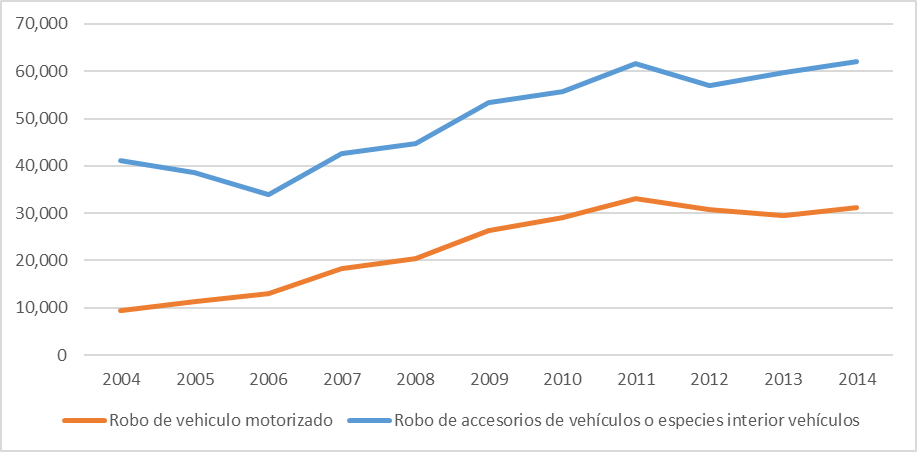
\includegraphics[width=0.45\textwidth]{business/cantidad_robos.png} &
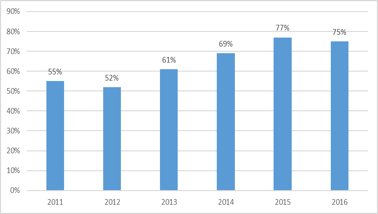
\includegraphics[width=0.40\textwidth]{business/tasa_robos_violencia.png}\\
\centering{(a)} & \centering{(b)}\\
\end{tabular}
\caption{(a) Cantidad de robos de vehículos y robos de accesorios de vehículos anuales en Chile (2004-2014). Fuente: Informe anual Carabineros, 2004-2014, INE. (b) Tasa de robos con violencia del total de robo de autos de lujo 2011-2016.} %Fuente?
\label{fig:antecedente}
\end{figure}

Bajo este contexto la Universidad de Chile junto a la Pontificia Universidad Católica de Chile se adjudicó el 2017 un proyecto Fondef para desarrollar un proyecto que lleva por nombre \quotes{Observatorio Digital de Delincuencia en Chile: Un sistema inteligente de apoyo a la industria automotriz chilena, en el robo de vehículos y accesorios} cuyo director es Richard Weber Haas y la institución beneficiaria es la Asociación de Aseguradores de Chile (AACH).\\

Para este problema se cuenta con las fuentes de datos de la AACH, lo que corresponde a relatos de las víctimas del robo de sus vehículos desde el 2011 hasta el 2016, lo cual corresponde a 49.015 relatos. Cabe destacar que se estima que un tercio del parque automotriz se encuentra asegurado, por lo que se trabaja con una muestra del parque automotriz.
%fuente

\section{Objetivo, Resultados esperados y Alcances}
El objetivo del trabajo de tesis es caracterizar los \textit{modus operandi} de los delincuentes a partir de los relatos de víctimas de robo de vehículo entregados por la AACH.\\

El resultado esperado es descubrir los \textit{modus operandi} ocultos en los relatos de las víctimas y caracterizarlos a partir de las palabras, como también ver su evolución a través del tiempo, siendo capaz de detectar cuando nacen y mueren, y como cambian en el tiempo.\\

El presente trabajo tiene un propósito académico, puesto que no cuenta con un cliente particular y tiene por objetivo estudiar ténicas de \textit{clustering} dinámico para detectar patrones en el contexto de robo de vehículos, sin embargo, potenciales beneficiarios del trabajo podrían ser las aseguradoras, los asegurados, carabineros de Chile y la sociedad.

\section{Metodología de trabajo}
%CRISP-DM
El trabajo se realizó bajo la metodología CRISP-DM (Cross Industry Standard Process for Data mining)\citep{chapman2000crisp}, la cual posee las siguientes seis etapas:
\begin{enumerate}
    \item Comprensión del negocio:
    %This initial phase focuses on understanding the project objectives and requirements from a business perspective, then converting this knowledge into a data mining problem definition and a preliminary plan designed to achieve the objectives.
    \item Comprensión de los datos
    %The data understanding phase starts with initial data collection and proceeds with activities that enable you to become familiar with the data, identify data quality problems, discover first insights into the data, and/or detect interesting subsets to form hypotheses regarding hidden information.
    \item Preparación de los datos
    %The data preparation phase covers all activities needed to construct the final dataset [data that will be fed into the modeling tool(s)] from the initial raw data. Data preparation tasks are likely to be performed multiple times and not in any prescribed order. Tasks include table, record, and attribute selection, as well as transformation and cleaning of data for modeling tools.
    \item Modelamiento
    %In this phase, various modeling techniques are selected and applied, and their parameters are calibrated to optimal values. Typically, there are several techniques for the same data mining problem type. Some techniques have specific requirements on the form of data. Therefore, going back to the data preparation phase is often necessary.
    \item Evaluación
    %At this stage in the project, you have built a model (or models) that appears to have high quality from a data analysisperspective. Before proceeding to final deployment of the model, it is important to thoroughly evaluate it and review the steps executed to create it, to be certain the model properly achieves the business objectives. A key objective isto determine if there is some important business issue that has not been sufficiently considered. At the end of this phase, a decision on the use of the data mining results should be reached.
    \item Implementación
    %Creation of the model is generally not the end of the project. Even if the purpose of the model is to increase knowledge of the data, the knowledge gained will need to be organized and presented in a way that the customer can use it. It often involves applying “live” models within an organization’s decision making processes—for example, real-time personalization of Web pages or repeated scoring of marketing databases. Depending on the requirements, the deployment phase can be as simple as generating a report or as complex as implementing a repeatable data mining process across the enterprise. In many cases, it is the customer, not the data analyst, who carries out the deploymen steps. However, even if the analyst will carry out the deployment effort, it is important for the customer to understand up front what actions need to be carried out in order to actually make use of the created models.
\end{enumerate}

Dentro de los alcances del trabajo no está contemplado la puesta en producción de una solución basada en \textit{machine learning}, el alcance es hasta la evaluación e interpretación de los resultados arrojados por el modelo.

\chapter{Revisión bibliográfica}

El problema planteado consiste en un problema de \textit{clustering}, puesto que no se cuenta con una etiqueta del \textit{modus operandi} al que corresponde cada relato, siendo el propósito del trabajo descubrirla. Dentro de los métodos de \textit{clustering} que involucran texto el modelamiento de tópicos es el enfoque más prometedor.% Fuente/Justificación
El modelamiento de tópicos es una herramienta estadística que busca encontrar los temas (tópicos) presentes en un conjunto de documentos (corpus), permitiendo organizar, buscar, indexar, explorar y comprender grandes colecciones de documentos. %Fuente
Los modelos de tópicos asumen que los documentos pueden ser representados por una mezcla de tópicos, donde los tópicos son distribuciones sobre las palabras, los tópicos son latentes y la inferencia tiene por objetivo descubrir la mezcla de tópicos que originó cada documento y la distribución sobre las palabras de cada tópico. En modelamiento de tópicos las personas son las que le dan una interpretación a los tópicos inferidos a partir de las palabras más relevantes y en base a esa información los etiquetan, por ejemplo, para un tópico, dentro de sus cinco palabras más probables se halla la siguiente secuencia: \quotes{llaves}, \quotes{domicilio}, \quotes{individuos}, \quotes{casa} y \quotes{portón}, una etiqueta valida para este tópico podría ser \quotes{portonazo}.\\

Algunas de las técnicas de modelamiento de tópicos están basadas en factorización matricial como LSI (Latent Semantic Indexing) \citep{dumais2004latent} o NMF (Non-negative Matrix Factorization)\citep{xu2003document}, pero en este trabajo se utilizarán técnicas basadas en modelos probabilísticos generativos, como LDA (Latent Dirichlet Allocation)\citep{blei2003latent} o HDP (Hierarchical Dirichlet Process)\citep{teh2005sharing}. Ambos enfoques tienen sus pros y contras, en este trabajo se prefiere el enfoque probabilísticos ya que es capaz de expresar incertidumbre en la asignación de un tópico a un documento y en la asignación de palabras a los tópicos, además, este enfoque suele aprender tópicos más descriptivos \citep{stevens2012exploring}.\\

El presente trabajo busca capturar el dinamismo que puede presentar el fenómeno del robo de vehículos. El aspecto dinámico del problema considera:
\begin{enumerate}
    \item Nacimiento, muerte, fusión y división de tópicos: En el contexto de robos es natural que en el tiempo aparezcan nuevos \textit{modus operandi} como también que desaparezcan aquellos que ya no parecen tan atractivos.
    \item Dinámismo en la mezcla de tópicos: esto permite capturar la popularidad de los tópicos en el tiempo.
    \item Evolución de los tópicos: la evolución de los tópicos se refleja en el cambio en la distribución sobre las palabras, esto permite detectar cambios en cómo se comete un mismo tipo de delito, por ejemplo, el \quotes{portonazo} en un determinado momento se comete en grupos de 2-3 personas con arma blanca, luego evoluciona de arma blanca a arma de fuego y lo perpetran jóvenes menores de edad.
\end{enumerate}

Dentro de los modelos de tópicos probabilísticos existen modelos estáticos y dinámicos:
\begin{enumerate}
    \item Dentro de los modelos estáticos destaca LDA y HDP. La diferencia principal en estos dos modelos es que el primero necesita de antemano fijar el número de tópicos a descubrir y el segundo lo infiere a partir del corpus.
    \item Dentro de los modelos dinámicos están aquellos que mantienen el número de tópicos fijos durante el tiempo y los que no:
    \begin{enumerate}
        \item En el primer grupo destaca Dynamic Topic Modelling (DTM)\citep{blei2006dynamic} junto Topic Over Time (TOC)\citep{wang2006topics}, la gran desventaja des estos modelos es que si aparece un nuevo tópico este quedará clasificado dentro de un tópico que existía desde el comienzo, por lo que solo es capaz de capturar el punto 2 y 3.
        \item Dentro de los modelos que no mantienen el número fijo de tópicos en el tiempo existen de dos tipos, aquellos que modelan todo el problema bajo un modelo monolítico, en este grupo destaca Dynamic Hierarchical Dirichlet Process (DHDP)\citep{ahmed2012timeline}, el cual modela el problema de dinamismo de una forma elegante pero a la vez acompañada de una inferencia bastante complicada, de los dinamismos mencionados captura los puntos 2, 3 y el 1 parcialmente, ya que no es capaz de capturar fusión y división de tópicos, uno de los principales contras de esta solución es que no se trata de una tecnología madura, puesto que no cuenta con una implementación disponible a diferencia de los otros modelos mencionados, los cuales se encuentran disponibles en múltiples lenguajes de programación y cuentan con una amplia adopción de la comunidad científica.El segundo tipo de modelos que no mantienen fijo el número de tópicos utilizan modelos de tópicos estáticos de forma iterativa, lo que hacen es dividir el corpus en épocas, luego entrenan de forma independiente un modelo de tópico para cada época y luego unen los resultados obtenidos, un ejemplo utilizando LDA en \citep{wilson2011tracking}  y con HDP en \citep{beykikhoshk2018discovering}.
    \end{enumerate}

En este trabajo se utilizarán técnicas de modelado dinámico de tópicos como las presentadas en \citep{wilson2011tracking,beykikhoshk2018discovering}, debido a que son capaces de modelar los tres puntos mencionados sobre dinamismo y se basan en tecnologías maduras.
\end{enumerate}

\chapter{Marco teórico}
\section{Modelos de tópicos}
%soft clustering vs hard clustering
\subsection{Latent Dirichlet Allocation}
\subsubsection{Distribución Dirichlet}
La distribución Dirichlet es una generalización multivariada de la distribución beta, la cual tiene soporte sobre un símplice, definido por:
\begin{equation}
    S_{K} = \{x: 0\leq x_{k} \leq 1, \sum_{k=1}^{K}x_{k}=1\}
\end{equation}
Luego, su función de densidad de probabilidad (pdf):

\begin{equation}
    Dir(x|\alpha)=\frac{1}{B(\alpha)}\prod_{k=1}^{K}x_{k}^{\alpha_{k}-1}
\end{equation}

La distribución Dirichlet es una distribución útil para generar distribuciones de probabilidades categóricas. En general se asume simetría en los parámetros de la distribución, es decir, $\alpha_{k}=\frac{\alpha}{K}$. En la Figura \ref{img:dirichlet_distribution} se observa el efecto de los parámetros de una Dirichlet en la muestra generada, para $\alpha_{k}=1$ se tiene una distribución uniforme en el dominio $S_{K}$, $\alpha_{k}$ controla la \textit{sparsity}, mientras más se acerca a 0 los vectores generados tienen más componentes nulos y se concentra la masa en unas pocas coordenadas, mientras más grande $\alpha_{k}$ la masa tiende a distribuirse uniformemente en las coordenadas de los vectores generados, por último, cuando $\alpha$ no es simétrico la masa se concentra en aquellas coordenadas cuyo $\alpha_{k}$ es más grande.

\begin{figure}
    \centering
    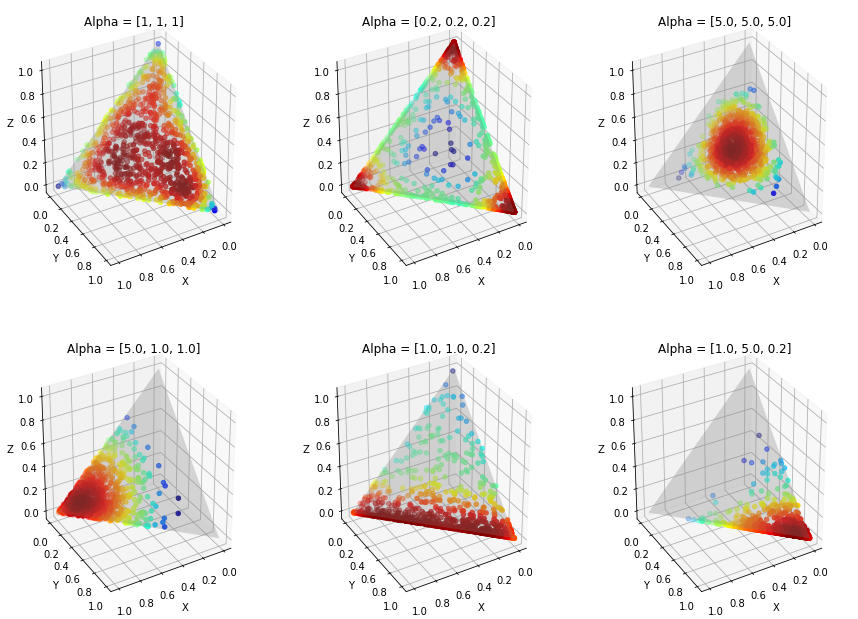
\includegraphics[width=1\textwidth]{math/dirichlet_distribution.png}
    \caption{Efecto de los parámetros de una distribución Dirichlet en el muestreo para $K=3$.}
    \label{img:dirichlet_distribution}
\end{figure}
% citar ilustración o crear
\subsubsection{LDA}
A continuación se describe el proceso generativo de Latent Dirichlet Allocation (LDA). Sean \textit{K} tópicos, $\phi_{1:K}$ distribuciones de probabilidad sobre un vocabulario fijo, dibujadas por una $Dir(\frac{\eta}{|V|}1_{|V|})$. Para cada documento $d$ del corpus $D$ se asume que es dibujado por el siguiente proceso generativo (ver representación gráfica del modelo en la Figura \ref{img:lda}):
\begin{enumerate}
    \item Dibujar una mezcla de tópicos $\pi_{d}\sim Dir(\frac{\alpha}{K}1_{K})$
    \item Para cada palabra:
    \begin{enumerate}
        \item Escoger un tópico $z_{d,n}\sim Mult(\pi_{d})$
        \item Escoger una palabra $w_{d,n}\sim Mult(\phi_{z_{d,n}})$
    \end{enumerate}
\end{enumerate}

\begin{figure}
  \centering
  \tikz{ %

    \node[latent, dashed] (alpha) {$\alpha$} ; %
    \node[latent, right=of alpha] (pi) {$\pi_{d}$} ; %
    \node[latent, right=of pi] (z) {$z_{d,n}$} ; %
    \node[obs, right=of z] (w) {$w_{d,n}$}   ; %
    \node[latent, right=of w] (phi) {$\phi_{k}$} ; %
    \node[latent, right=of phi, dashed] (eta) {$\eta$} ;%
    \plate[inner sep=0.25cm, xshift=-0.12cm, yshift=0.12cm] {plate1} {(z) (w)} {$N_{d}$}; %
    \plate[inner sep=0.25cm, xshift=-0.12cm, yshift=0.12cm] {plate2} {(pi) (plate1)} {$D$}; %
    \plate[inner sep=0.25cm, xshift=-0.12cm, yshift=0.12cm] {plate3} {(phi)} {$K$}; %
    \edge {alpha} {pi} ; %
    \edge {pi} {z} ; %
    \edge {z,phi} {w} ; %
    \edge {eta} {phi} ; %
  }
\caption{Representación gráfica de LDA: círculos denotan variables aleatorias, círculos abiertos denotan parámetros, círculos sombreados denotan variables observadas y los platos indican replicación.}
\label{img:lda}
\end{figure}

La probabilidad conjunta del modelo:
\begin{equation}
    p(\phi, \pi, z, w|\alpha, \eta)= \prod_{k=1}^{K}p(\phi_{k}|\eta)\prod_{d=1}^{D}p(\pi_{d}|\alpha)\prod_{n=1}^{N_{d}}p(z_{n,d}|\pi_{d})p(w_{d,n}|\phi_{1:K}, z_{d,n})
\end{equation}

La distribución a posterior:
\begin{equation}
    p(\phi, \pi, z|w, \alpha, \eta) = \frac{p(\phi, \pi, z, w|\alpha, \eta)}{p(w|\alpha, \eta)}
\end{equation}

La distribución posterior es computacionalmente intratable para inferencia exacta, debido a que para normalizar la distribución debemos marginalizar sobre todas las variables ocultas y escribir la constante de normalización en términos de los parámetros del modelo. Para poder computar la posterior es necesario utilizar algoritmos de inferencia aproximada, donde el enfoque habitual es Markov Chain Monte Carlo (MCMC), en \citep{griffiths2004finding} se propone un algoritmo basado en Gibbs Sampling para la inferencia. Los métodos basados en MCMC entregan una estimación empírica de la distribución posterior llamada (traza), es decir, representan la posterior a través de muestras que distribuyen como esta, luego para estimación puntual, como por ejemplo obtener el valor esperado de la posterior se utiliza integración de Monte Carlo para aproximar la esperanza, esto es promediar los valores de la traza.

\subsection{Hierarchical Dirichlet Process}
\subsubsection{Proceso Dirichlet}

En los modelos probabilísticos de \textit{clustering} existen aquellos basados en mezcla finita de componentes que utilizan como \textit{prior} la distribución Dirichlet y aquellos basados en mezcla infinita de componentes que utilizan como \textit{prior} el proceso Dirichlet, un \textit{prior} no paramétrico que no impone una cota en el número de \textit{clusters} a encontrar ($K$).\\

Una representación equivalente en LDA sería generar cada palabra de un documento $d$ a partir de una multinomial sobre un tópico dibujado por una distribución $G_{d}$, formalmente, $w_{d,n}\sim Mult(\phi_{d,n})$, donde $\phi_{d,n} \sim G_{d}$ con $\phi_{d,n} \in \{\phi_{k}\}_{k=1}^{K}$, y $G_{d}(\phi)=\sum_{k=1}^{K}\pi_{d, k}\delta_{\phi_{k}}(\phi)$, donde $\delta_{\phi_{k}}(\phi) = \begin{cases}
    1 & \text{si $\phi_{k}=\phi$}  \\
    0 & \text{si no}
  \end{cases}$.\\\\

Un proceso Dirichlet (DP) es una distribución sobre medidas de probabilidad $G: \Theta \rightarrow \mathbf{R}^{+}$, donde $G(\theta)\geq 0$ y $\int_{\Theta}G(\theta)d\theta=1$. Un DP se define implícitamente por cumplir que para cualquier partición finita $(T_{1}, \ldots, T_{k})$ de $\Theta$, una medida base $H$ y un parámetro de concentración $\alpha$ se  tiene que $(G(T_{1}), \ldots, G(T_{K})) \sim Dir(\alpha H(T_{1}), \ldots, \alpha H(T_{k}))$.

\subsubsubsection{Stick breaking construction}
En esta sección describiremos una construcción para el DP conocida como \textit{stick breaking construction}. Sea $\pi=\{\pi_{k}\}_{k=1}^{\infty}$ una secuencia de mezcla de pesos derivadas a partir del siguiente proceso:
\begin{equation}
    \beta_{k}\sim Beta(1, \alpha)
\end{equation}
\begin{equation}
    \pi_{k} = \beta_{k}\prod_{l=1}^{k-1}(1-\beta_{l}) = \beta_{k}(1-\sum_{l=1}^{k-1}\pi_{l})
\end{equation}

Esto se suele denotar como $\pi \sim GEM(\alpha)$, donde GEM representa Griffiths, Engen y McCloskey. Algunos ejemplos de este proceso son mostrados en la Figura \ref{img:stick_breaking}.

\begin{figure}
    \centering
    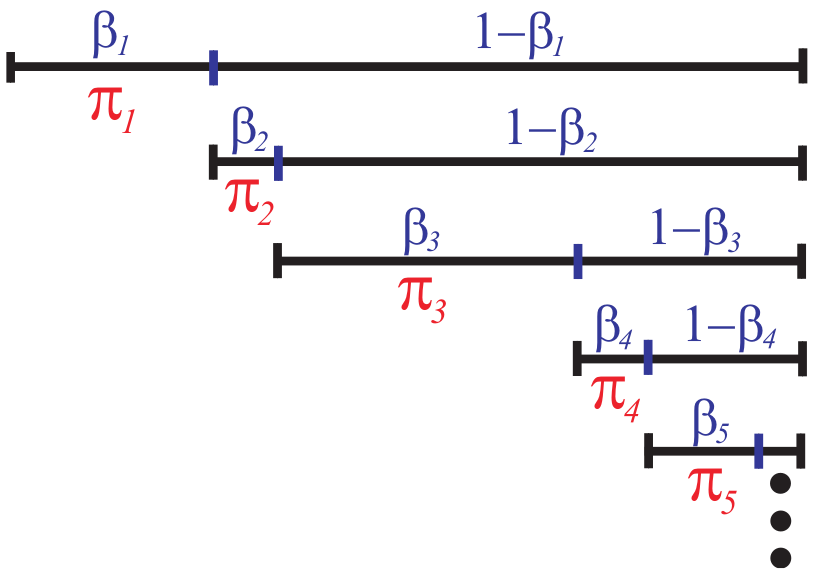
\includegraphics[width=1\textwidth]{math/stick_breaking.png}
    \caption{Ilustración de \textit{stick breaking construction}. (a) Tenemos una barra de largo 1, el cual se rompe en un punto aleatorio $\beta_{1}$, el largo de la pieza que conservamos es llamada $\pi_{1}$, luego recursivamente rompemos la barra restante, así generando $\pi_{2}, \pi_{3}, \ldots$. (b) Muestras de $\pi_{k}$ para $\alpha=2$ y $\alpha=5$.}
    \label{img:stick_breaking}
\end{figure}
% citar ilustración

Se puede demostrar que este proceso terminará con probabilidad 1 (convergencia casi segura), a pesar que el número de elementos que este genera incrementa con $\alpha$. Además, el tamaño del componente $\pi_{k}$ decrece en promedio.
Ahora definamos

\begin{equation}
    G(\phi) = \sum_{k=1}^{\infty}\pi_{k}\delta_{\phi_{k}}(\phi)
\end{equation}
donde $\pi \sim GEM(\alpha)$ y $\phi_{k} \sim H$, se puede demostrar que $G \sim DP(\alpha, H)$. Como consecuencia de esta construcción, las muestras de un DP son discretas con probabilidad uno. En otras palabras, al ir muestreando se tendrán mas repeticiones de valores generados previamente, por lo que la mayoría de los datos vendrán de los $\phi_{k}$ con $\pi_{k}$ mayor.

\subsubsection{HDP}

Hierarchical Dirichlet Process (HDP) es una colección de DP que comparten una distribución base $G_{0}$, la cual además es dibujada a partir de un DP (ver representación gráfica del modelo en la Figura \ref{img:hdp}). Matemáticamente, a nivel corpus se tiene que la distribución base $H \sim Dir(\frac{1}{|V|}1_{|V|})$ y $G_{0} \sim DP(\gamma, H)$, luego, para cada documento $d$ del corpus $D$ se asume que es dibujado por el siguiente proceso generativo:
\begin{enumerate}
    \item Dibujar un DP $G_{d} \sim DP(\alpha_{0}, G_{0})$
    \item Para cada palabra:
    \begin{enumerate}
        \item Dibujar un tópico $\phi_{d,n}\sim G_{d}$
        \item Escoger una palabra $w_{d,n} \sim Mult(\phi_{d,n})$
    \end{enumerate}
\end{enumerate}

\begin{figure}
  \centering
  \tikz{ %
    \node[latent, dashed] (H) {$H$} ; %
    \node[latent, right=of H] (G0) {$G_{0}$} ; %
    \node[latent, above= of G0, dashed] (gamma) {$\gamma$} ; %
    \node[latent, right=of G0] (Gd) {$G_{d}$} ; %
    \node[latent, above= of Gd, dashed] (alpha0) {$\alpha_{0}$} ; %
    \node[latent, right= of Gd] (phi) {$\phi_{d,n}$} ; %
    \node[obs, right=of phi] (w) {$w_{d,n}$}   ; %
    \plate[inner sep=0.25cm, xshift=-0.12cm, yshift=0.12cm] {plate1} {(phi) (w)} {$N_{d}$}; %
    \plate[inner sep=0.25cm, xshift=-0.12cm, yshift=0.12cm] {plate2} {(Gd) (plate1)} {$D$}; %
    \edge {H, gamma} {G0} ; %
    \edge {G0, alpha0} {Gd} ; %
    \edge {Gd} {phi} ; %
    \edge {phi} {w} ; %
  }
\caption{Representación gráfica de HDP: círculos denotan variables aleatorias, círculos abiertos denotan parámetros, círculos sombreados denotan variables observadas y los platos indican replicación.}
\label{img:hdp}
\end{figure}

La discretitud a nivel corpus de $G_{0}$ asegura que todos los documentos comparten el mismo conjunto de tópicos (\textit{mixture components}). A nivel documento $G_{d}$ hereda los tópicos de $G_{0}$, pero los pesos de cada tópico (\textit{mixture proportions}) es específica del documento.\\

Aplicando \textit{stick breaking construction} se tiene que para el DP dibujado a nivel corpus la siguiente representación:

\begin{align}
    \beta_{k}^{'} \sim Beta(1, \gamma) \\
    \beta_{k} = \beta_{k}^{'}\prod_{l=1}^{k-1}(1-\beta_{l}^{'})\\
    \phi_{k} \sim H  \\
    G_{0}(\phi)=\sum_{k=1}^{\infty}\beta_{k}\delta_{\phi_{k}}(\phi)
\end{align}


Así, $G_{0}$ es discreto y tiene soporte en los átomos $\phi = \{\phi\}_{k=1}^{\infty}$ con pesos $\beta=\{\beta_{k}\}_{k=1}^{\infty}$, siendo la distribución de $\beta$ escrita como $\beta \sim GEM(\gamma)$. La construcción a nivel documento de $G_{d}$ es:

\begin{align}
    \pi_{d,k}^{'}\sim Beta\big(\alpha_{0}\beta_{k}, \alpha_{0}\big(1-\sum_{l=1}^{k}\beta_{l}\big)\big)\\
    \pi_{d,k} = \pi_{d,k}^{'}\prod_{l=1}^{k-1}(1-\pi_{d,l}^{'})\\
    G_{d}(\phi)=\sum_{k=1}^{\infty}\pi_{d,k}\delta_{\phi_{k}}(\phi)
\end{align}

Donde $\phi = \{\phi_{k}\}_{k=1}^{\infty}$ son los mismos átomos de $G_{0}$. En la Figura \ref{img:hdp_sbc} se muestra la representación gráfica de esta construcción.

%stick breaking
\begin{figure}
  \centering
  \tikz{ %
    \node[latent] (beta) {$\beta$} ; %
    \node[latent, above= of beta, dashed] (gamma) {$\gamma$} ; %
    \node[latent, right=of beta] (pi) {$\pi_{d}$} ; %
    \node[latent, above= of pi, dashed] (alpha0) {$\alpha_{0}$} ; %
    \node[latent, right= of pi] (z) {$z_{d,n}$} ; %
    \node[obs, right=of z] (w) {$w_{d,n}$}   ; %
    \node[latent, right=of w] (phi) {$\phi$} ; %
    \node[latent, above=of phi, dashed] (H) {$H$} ; %
    \plate[inner sep=0.25cm, xshift=-0.12cm, yshift=0.12cm] {plate1} {(z) (w)} {$N_{d}$}; %
    \plate[inner sep=0.25cm, xshift=-0.12cm, yshift=0.12cm] {plate2} {(pi) (plate1)} {$D$}; %
    \plate[inner sep=0.25cm, xshift=-0.12cm, yshift=0.12cm] {plate3} {(phi)} {$K (\infty)$}; %
    \edge {gamma} {beta} ; %
    \edge {beta, alpha0} {pi} ; %
    \edge {pi} {z} ; %
    \edge {z, phi} {w} ; %
    \edge {H} {phi} ; %
  }
\caption{Representación gráfica de la construcción stick-breaking de HDP: circulos denotan variables aleatorias, circulos abiertos denotan parámetros, círculos sombreados denotan variables observadas y los platos indican replicación.}
\label{img:hdp_sbc}
\end{figure}

Al igual que LDA la distribución posterior es intratable, por lo que en \citep{teh2005sharing} se marginaliza $G_{0}$ y $G_{d}$'s afuera, obteniéndose así un nuevo proceso generativo denominado \textit{Chinese restaurant franchise process} (CRF), esta representación permite construir algoritmos eficientes basados en Gibbs Sampling, como en la implementación utilizada disponible en \citep{HDP}.

\subsubsection{LDA versus HDP}
HDP es un modelo no paramétrico similar en estructura a LDA, la principal desventaja de LDA frente a HDP es que LDA requiere escoger el número de tópicos $K$ por adelantado, por otro lado, en HDP el número de tópicos no está acotado y es inferido a partir de los datos. En un enfoque tradicional, se requiere de entrenar múltiples veces LDA para diferentes valores de $K$ y se escoge el que tiene mejor la configuración con mejor desempeño en un conjunto de validación, por lo que LDA termina siendo computacionalmente más costoso que HDP, además este enfoque se vuelve impracticable cuando el conjunto de datos es grande. En el aspecto cualitativo ambos modelos entregan tópicos igual de consistentes, en cuanto a métricas de desempeño como $\textit{perplexity}$ HDP suele tener mejor desempeño \citep{teh2005sharing}.

\subsection{Interpretación de tópicos}
Los modelos de tópicos se caracterizan por tener un alto poder interpretativo, esto se debe a que la distribución de probabilidad de cada tópico sobre el vocabulario nos da una idea del tema al que pertenece, por otro lado la mezcla de tópicos de cada documento muestra que tan importante es cada tópico en la generación de estos, como también dentro del corpus. En este sentido, las visualizaciones nos ayudan a interpretar mejor los resultados de los modelos de tópicos, respondiendo a las siguientes preguntas, ¿Cuál es el significado de cada tópico?¿Cuán predonimnante es cada tópico?¿Cómo se relacionan los tópicos entre sí?\\

En \citep{sievert2014ldavis} desarrollaron una herramienta de visualización web para responder a estas preguntas. Para responder la pregunta 1 se incorpora un gráfico de barras que muestra las palabras más relevantes del tópico seleccionado dado un parámetro $\lambda \in [0,1]$. A través de una visualización espacial responde la pregunta 2 y 3. La visualización espacial consiste en aplicar técnicas de reducción de dimensionalidad como TSNE \citep{maaten2008visualizing} o PCA \citep{wold1987principal} (en este caso se utilizó TSNE) a la matriz de distancia entre tópicos, usando Jensen-Shannon divergence \citep{endres2003new} como médida de distancia. Una vez cada tópico es mapeado a un punto en un espacio de dos dimensiones se dibuja un círculo con centro en este punto y con radio proporcional a la cantidad de tokens generados por el tópico.\\

Para interpretar un tópico, uno típicamente examina una lista ordenada de los palabras más probables en el tópico, usando ya sea desde cinco a treinta términos. Un problema frecuente que se presenta en este caso es que los términos que son comunes al corpus frecuentemente aparecen en el top de las palabras más probables de un tópico, haciendo difícil discernir el significado de estos.
Para esto en \citep{sievert2014ldavis} se define una métrica denominada \textit{relevance}, la cual define la relevancia de una palabra no solo por su probabilidad dentro del tópico sino también por su exclusivad dentro del corpus. La \textit{relevance} de una palabra $w$ en el tópico $k$ dado $\lambda$ está dada a través de la siguiente expresión:

\begin{align}
    r(w,k|\lambda) = \lambda log (\phi_{kw})+ (1-\lambda)\lambda log\bigg(\frac{\phi_{kw}}{p_{w}}\bigg)
\end{align}

, donde $\lambda$ determina el peso que se le da a la probabilidad de la palabra $w$ dentro del tópico $k$ ($\phi_{kw}$) relativo a su \textit{lift}, el cual se define por el ratio entre la probabilidad de la palabra dentro del tópico y su probabilidad marginal a lo largo del corpus ($p_w$). Fijando $\lambda=1$ se obtiene el ranking de términos decrecientes en orden de su probabilidad dentro del tópico, y fijando $\lambda=0$ el ranking se basa solo en el \textit{lift}.

\section{Modelamiento de la evolución de los tópicos en el tiempo}

Nuestro objetivo es modelar la evolución en el tiempo de los tópicos, para esto el corpus es divido en $T$ épocas, en cada época se entrena un modelo de tópicos estático, obteniéndose así $T$ conjuntos de tópicos $\phi=\{\phi_{1}, \ldots, \phi_{T}\}$, donde $\phi_{t}=\{\phi_{t,1}, \ldots, \phi_{t,K_{t}}\}$ es el conjunto de tópicos que describen la época $t$, y $K_{t}$ el número de tópicos inferido en esa época.

\subsection{Gráfo de similitud temporal}
Para relacionar los tópicos de una época necesitamos una medida de similitud $\rho \in [0,1]$, con esta médida de similitud se puede construir un gráfo, donde los nodos son los tópicos de una época y los arcos relacionan tópicos de una época con la siguiente, siendo el peso del arco la similitud entre los tópicos. Una vez construido el grafo se eliminan las conexiones débiles en base a un umbral $\zeta \in [0,1]$ a definir, reteniendo solo aquellas conexiones entre tópicos suficientemente similares entre épocas adyacentes, matemáticamente podamos el arco entre los tópicos $\phi_{t,i}$ y $\phi_{t+1,j}$ si $\rho(\phi_{t,i}, \phi_{t+1,j})\leq \zeta$. Una ilustración conceptual del grafo de similitud es mostrado en la Figura \ref{img:graph}, este muestra tres épocas consecutivas.

\begin{figure}
    \centering
    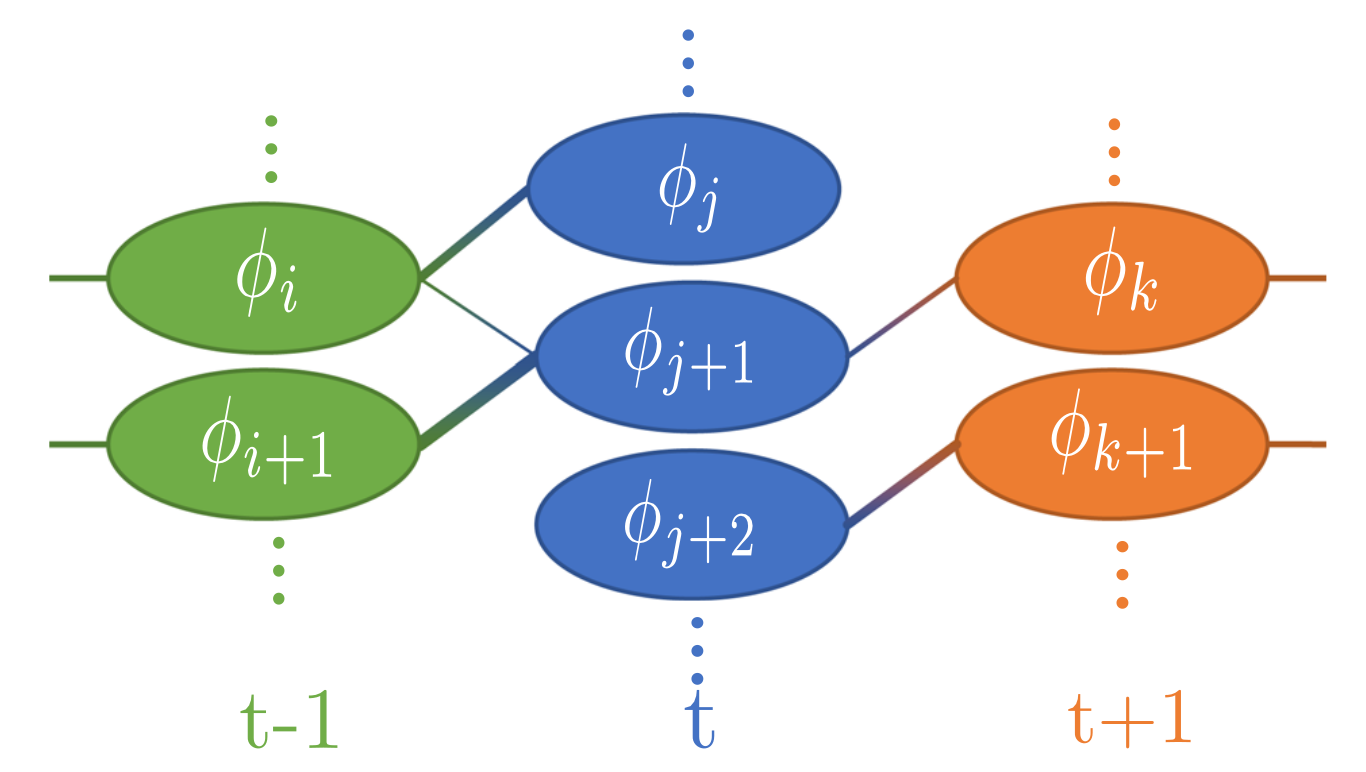
\includegraphics[width=0.8\textwidth]{math/similarity_graph.png}
    \caption{Ilustración conceptual del grafo de similitud que modela la dinámica de los tópicos en el tiempo. Un nodo corresponde a un tópico en una época específica; el ancho de los arcos es proporcional a la similitud entre los tópicos, arcos ausentes fueron eliminados por presentar una similitud menor a un umbral.}
    \label{img:graph}
\end{figure}

Está metodología permite fácilmente detectar desaparición de un tópico, nacimiento de un nuevo tópico, como también dividir o fusionar diferentes tópicos, a continuación se define en detalle cada uno de estos dinamismos:

\begin{itemize}
    \item \textbf{Nacimiento de un tópico:} Si un tópico no tiene ningún arco entrante, por ejemplo, en la Figura \ref{img:graph} el tópico $\phi_{j+2}$ en $t$.
    \item \textbf{Muerte de un tópico:} Si un tópico no tiene ningún arco saliente, por ejemplo, en la Figura \ref{img:graph} el tópico $\phi_{j}$ en $t$.
    \item \textbf{Evolución de un tópico:} Cuando un tópico tiene exactamente un arco de entrada y salida, por ejemplo, en la Figura \ref{img:graph} entre las épocas $t$ y $t+1$ se tiene que el tópico $\phi_{j+2}$ evoluciona del tópico $\phi_{k+1}$.
    \item \textbf{División de un tópico:} Si un tópico tiene más de un arco saliente, por ejemplo, en la Figura \ref{img:graph} el tópico $\phi_{i}$ de $t-1$ se divide en $t+1$ en los tópicos $\phi_{j}$ y $\phi_{j+1}$.
    \item \textbf{Fusión de un tópico:} Cuando un tópico tiene más de un arco entrante, este tipo de tópicos también pueden ser entendidos como un nuevo tópico, por ejemplo, en la Figura \ref{img:graph} los tópicos $\phi_{i}$ y $\phi_{i+1}$ de $t-1$ forman al tópico $\phi_{j+1}$ en $t$.
\end{itemize}

Un aspecto relevante de esta metodología es definir el úmbral de corte, el cual no es fácilmente interpretable, además el úmbral depende de la médida de similitud escogida, dificultando así la comparación entre médidas de similitud. En \cite{beykikhoshk2018discovering} proponen una alternativa más interpretable para definir el úmbral, para esto estiman la función de distribución acumulada (cdf) del grafo inicial, donde todos los nodos de una época están conectados con todos los nodos de la época adyacente, sea $F_{p}$ la cdf sobre las similitudes del grafo inicial, luego sea $\zeta \in [0,1]$ el punto operante de la cdf, luego eliminamos el arco entre los tópicos $\phi_{t,i}$ y $\phi_{t+1,j}$ si $\rho(\phi_{t,i}, \phi_{t+1,j})\leq F_{p}^{-1}(\zeta)$, donde  $F_{p}^{-1}(\zeta)$ es el cuantil $\zeta$ de $F_{p}$.

\subsection{Medidas de similitud}
Los tópicos son distribuciones de probabilidad sobre un vocabulario fijos de términos. La gran mayoría de medidas de similitud comparan vectores con el mismo dominio y dimensión, esto significa que los tópicos de épocas adyacentes deben compartir el mismo vocabulario, matemáticamente, sea $\phi_{t, i}$ un tópico de la época $t$ y $V_{t}$ su vocabulario, sea  $\phi_{t+1, j}$ un tópico de la época $t+1$ y $V_{t+1}$ su vocabulario, lo más probables es que existan palabras en $V_{t}$ que no existan en $V_{t+1}$ y viceversa, para poder comparar tópicos en estas épocas adyacentes se debe construir el vocabulario $V_{t+1}^{'}=V_{t}\cup V_{t+1}$, luego se aplica $padding$ a los vectores $\phi_{t, i}$ y $\phi_{t+1, j}$, es decir, se rellenan con ceros las posiciones de palabras que no están en el vocabulario de su dominio.\\

La gran desventaja del enfoque anterior es que no captura similitud entre palabras, es decir, dos palabras diferentes que pueden llegar a ser sinónimos ocuparan una posición diferente dentro del vector, siendo no robusta a cuando una palabra esta presente en la época $t$ y no en $t-1$ por lo que no hay forma de compararla por ejemplo con la palabra de $t-1$ más símil, por lo que se compara la palabra consigo misma, donde en $t$ tiene un peso distinto de cero y en $t-1$ un peso nulo. El peor caso sería considerar los vocabularios $V_{t}$ y $V_{t+1}$, donde $V_{t}\cap V_{t+1} =  \emptyset$, a pesar de que cada palabra en $V_{t}$ tiene un sinónimo en $V_{t+1}$ la similitud entre tópicos entre las épocas $t$ y $t+1$ sería cero.\\

Para lidiar con el problema anterior en \citep{kusner2015word} se propone una medida de distancia llamada Word Mover's Distance (WMD) para comparar dos documento bajo una representación \textit{bag of words}, donde $i$ y $j$ son los documentos, $V_{i}$ y $V_{j}$ los vocabularios, y el peso asociado a cada palabra de un documento  es igual a la frecuencia normalizada. Generalizar al caso de tópicos es bastante sencillo, puesto a que estos se construyen bajo una representación bag of words, por ejemplo, para comparar el tópico $i$ de la época $t$ con el tópico $j$ de la época $t+1$, se usan los pesos $\phi_{t,i}$ y $\phi_{t+1,j}$ sobre el vocabulario $V_{t}$ y $V_{t+1}$ respectivamente. WMD calcula el costo mínimo de transformar un documento en otro, en esto caso particular sería el costo mínimo de llevar un tópico a otro, para esto se resuelve el problema de transporte, donde los flujos son los pesos $\phi_{t,i}$ y $\phi_{t+1,j}$ y la matriz de costos es una matriz de distancia euclidiana entre los \textit{word embedding} (\cite{mikolov2013distributed}) de todas las palabras de $V_{t}$ con $V_{t+1}$. Para resolver este problema se utilizó la implementación de \citep{PyEMD}. En la Figura \ref{img:wmd_obama} se ilustra el espacio en el que viven las palabras de dos tópicos.

\begin{figure}
    \centering
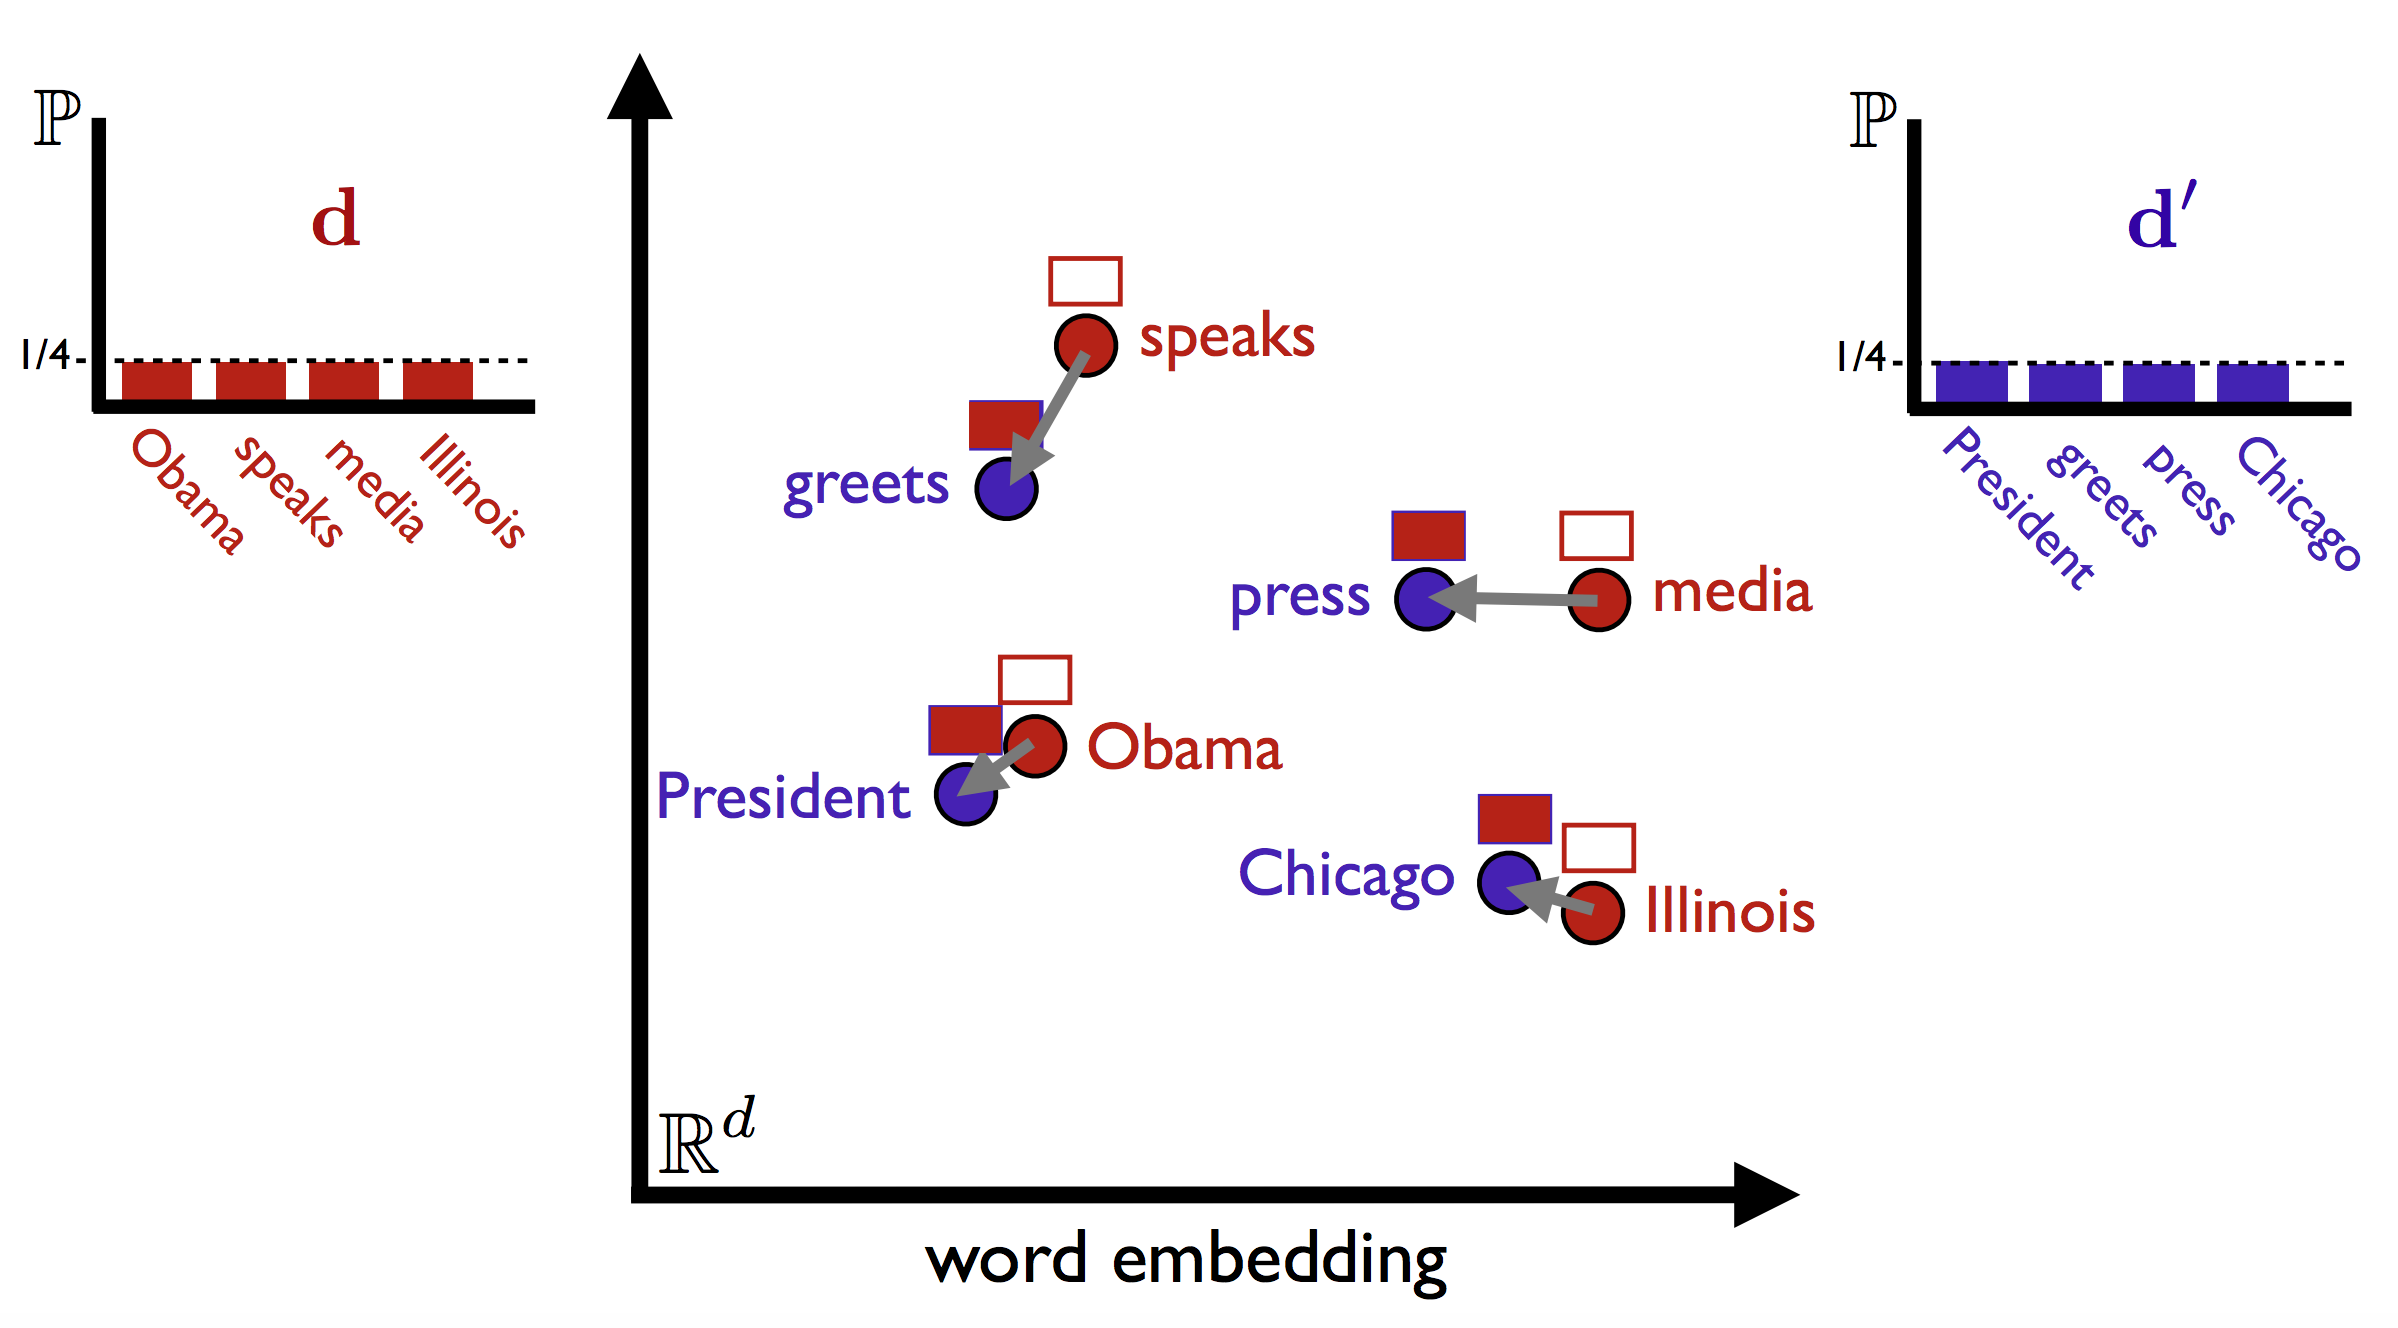
\includegraphics[width=1\textwidth]{math/wmd-obama.png}
    \caption{Espacio vectorial de los \textit{word embeddings} de las palabras de dos tópicos con un vocabulario de tamaño 4.}
    \label{img:wmd_obama}
\end{figure}

Matemáticamente, la WMD entre el tópico $i$ de la época $t$ y el tópico $j$ de la época $t+1$ viene dado por $WMD(\phi_{i,t}, \phi_{j,t+1})$:

\begin{align}
\underset{T}{\text{minimize}}&\sum_{u \in V_{t}}\sum_{v \in V_{t+1}} c_{u,v}T_{u,v} \\ 
\textrm{s.t.}\qquad &\sum_{v \in V_{t+1}}T_{u,v}= \phi_{i,t,u} \;, u \in V_{t}\\ 
& \sum_{u \in V_{t}}T_{u,v}= \phi_{j,t+1,v} \;, v\in V_{t+1}\\
& T_{u,v} \geq 0,\; u \in V_{t} \;, v \in V_{t+1}\\ \nonumber
\end{align}

Donde $T_{u,v}$ es el flujo que va de la palabra $u$ del tópico $i$ de la época $t$ a la palabra $v$ del tópico $j$ de la época $t+1$, $\phi_{i,t,u}$, es la probabilidad de la palabra $u$ en el tópico $i$ de la época $t$, $c_{u,v}$ es el costo de mover una unidad de flujo por el arco $(u,v)$, el costo entre palabras se mide como la distancia euclidiana entre los \textit{word embedding} de dichas palabras. La primera restricción indica que el flujo que se mueve de una palabra $u$ del tópico $i$ a todas las palabras del tópico $j$ debe sumar su peso ($\phi_{i,t,u}$), la segunda restricción significa que el flujo que se mueve de una palabra $v$ del tópico $j$ a todas las palabras del tópico $i$ debe sumar su peso ($\phi_{j,t+1,v}$). Esta médida de distancia se puede fácilmente transformar en una médida de similitud $\rho(\phi_{i,t}, \phi_{j,t+1}) = \frac{1}{1+WMD(\phi_{i,t}, \phi_{j,t+1})}$, notar que si la WMD es 0 la similitud es 1 y si es $\infty$ la similitud es 0. \\

WMD es una medida de distancia intensiva en recursos computacionales, para entender mejor esto utilizaremos la representación poliedral del problema, sea $N$ el tamaño del vocabulario entre dos épocas adyacentes, luego la región factible del problema anterior se puede representar como $\{x| Ax=b, x\geq 0\}$, con $A\in \mathbb{R}^{2N\times N^{2}}$ la matriz de costos, $b\in \mathbb{R}^{2N}$ el flujo disponible y $x\in \mathbb{R}^{N}$ el flujo a enviar por cada uno de los arcos, la complejidad del mejor tiempo promedio de resolver este problema de optimización escala $\mathcal{O}(N^{2}log N)$ \citep{pele2009fast}, por lo que si se reduce el vocabulario a un décimo esto trae una reducción de al menos unas 200 veces (en el peor caso promedio). Los tópicos siguen una distribución de ley de potencia sobre el vocabulario, donde una fracción de las palabras concentran la mayor parte de la masa de la distribución. Además, en la práctica la interpretación de los tópicos se basa en los top $T$ palabras más probables (o relevantes) con $T \in [5, 30]$, entonces, podemos aprovechar esta estructura para efectos de computar la WMD de un forma más eficiente, por ejemplo, utilizando solo las palabras que capturan un 95\% de la distribución acumulada del tópico.

\chapter{Experimento}

\section{Datos}

Para este experimento se cuenta con las fuentes de datos de la Asociación de Aseguradores de Chile (AACH), corresponde a los relatos que las víctimas del robo de sus vehículos dan a las aseguradoras, lo cual corresponde a 49.015 relatos entre el 2011 y 2016.\\

% descripción detallada del conjunto de datos
% gráficos del Informe_1_fondef?
% hablar del nivel de granularidad, justificar en base facilidad de análisis de resultados, interpretación, largo del grafo, combinatoria, etc


Para el uso de WMD es necesario contar con \textit{words embeddings}, para esto se utilizaron los \textit{embeddings} de \citep{fastextSBWC}, estos \textit{embeddings} fueron obtenidos utilizando el algoritmo FastText \citep{bojanowski2017enriching} sobre el corpus Spanish Billion Word Corpus (SBWC) \citep{cardellinoSBWCE}. FasText en comparación a otros enfoques para extraer \textit{embeddings} representa los \textit{tokens} a través de n-gramas de caracteres, de esta manera se pueden obtener \textit{embeddings} de \textit{tokens} no vistos durante el entrenamiento a partir de los \textit{embeddings} de los caracteres que lo componen.

\section{Procesamiento}

En minería de texto con el objetivo de extraer el core de palabras del corpus se recurre métodos para reducir el vocabulario, la reducción del vocabulario mejora la significancia estadística de los modelos, puesto que se obtiene un mejor balance entre cantidad de parámetros y cantidad de observaciones, por otro lado puede verse fácilitada la interpretación de los tópicos al remover palabras que aportan poca información. \\

El paso cero en el procesamiento de textos es tokenizar, la tokenización es una operación sobre una cadena de carácteres (\textit{string}) que consiste en dividir el \textit{string} en un conjunto de términos, en este caso la división se hizo por el carácter espacio, como resultado de esto se obtiene una lista de elementos, a cada elemento de esta lista se le denomina \textit{token} que en términos simples puede considerarse como una palabra para el ejemplo mencionado. \\

Luego, en el primer nivel de procesamiento no interesa hacer distinción entre mayúsculas o minúsculas\footnote{En análisis de sentimiento puede ser interesante ya que las personas suelen expresar mensajes de enfado con letras capitales, por lo que las letras capitales añaden información al análisis.}, por ende, los carácteres de cada token son llevados a minúscula, también se eliminaron carácteres y tokens que no aportan información, como símbolos de puntuación, correos electrónicos y tokens que contienen números. En la figura \ref{img:cum_dist1} se observa la distribución acumulada de los tokens del corpus a este nivel de procesamiento, adicionalmente se tiene que el 50\% de los \textit{tokens} del vocabulario ocurren una sola vez, el 80\% tiene una ocurrencia menor o igual a 5 y el 95\% de la distribución acumulada puede ser explicada con 4199 \textit{tokens} (9\%) del vocabulario, se concluye que la distribución es sumamente pesada y es necesario recurrir a métodos adicionales para su reducción.\\

\begin{figure}
    \centering
    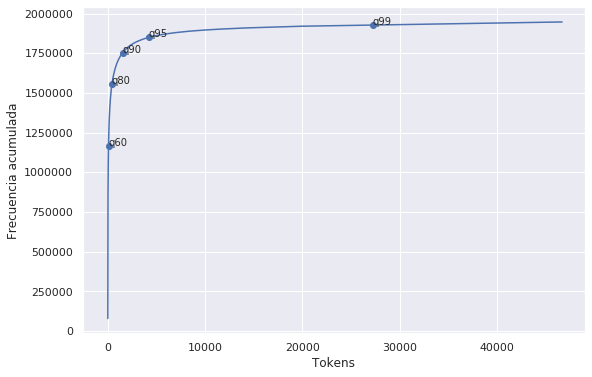
\includegraphics[width=0.8\textwidth]{experiments/cum_dist_1.png}
    \caption{Frecuencia acumulada de los tokens únicos aplicando hasta el primer nivel de procesamiento. El eje horizontal es el acumulado de tokens únicos en orden decreciente de ocurrencia. Los puntos corresponden a los cuantiles 60\%, 80\%, 90\%, 95\% y 99\%.}
    \label{img:cum_dist1}
\end{figure}

En el segundo nivel de procesamiento se eliminaron las \texit{stopwords}, palabras que aportan poca información, como artículos, preposiciones y conectores, para esto se utilizó la lista de \textit{stopwords} disponible en el paquete NLTK de Python \citep{bird2009natural} la cual cuenta con 313 palabras. Además, esta lista de \textit{stopwords} se alimentó con \textit{stopwords} contextuales, palabras específicas del corpus que aportan poca información, para esto se hizó un etiquetado de las 1000 palabras más frecuentes del corpus incorporando 417 nuevas palabras, algunos ejemplos son palabras que hacen referencia a vehículo y robo, puesto que todos los documentos corresponden a robos de vehículos.\\

El tercer nivel de procesamiento consiste en normalizar los tokens para reducir aún más el vocabulario, como métodos de normalización los más utilizados son \textit{stemming}  y lematización. \textit{Stemming} es el proceso de llevar una palabra a su raíz (\textit{stem}), en la práctica \textit{stemming} consiste en aplicar un algoritmo basado en ciertas reglas gramáticales para extraer sufijos \citep{porter1980algorithm}, como desventaja es que stemming no tiene en cuenta el contexto de la palabra por lo que la raíz obtenida puede no corresponder a la raíz verdadera de la palabra, además, para el caso de modelamiento de tópicos los tópicos se vuelve más difícil de interpretar, ya que palabras con significado completamente distinto terminan con la misma raíz o bien la raíz encontrada no tiene un significado claro. Por otro lado, lematización es el proceso de agrupar juntas las formas flexionadas de una palabra para que puedan analizarse como un elemento, identificado como lema, su diferencia principal con \textit{stemming} es que opera con conocimiento del contexto de la palabra para discriminar entre palabras que tienen significado diferente dependiendo del \textit{part of speech tagging} (POST) y de una tabla de búsqueda (\textit{lookup table}). Como método de normalización se decidió utilizar lematización en vez de \texit{stemming} debido a que tiene menos impacto en la interpretación de los tópicos, sin embargo es una operación más intensiva debido a que \texit{stemming} es un algoritmo basado en reglas simples mientras que en lematización se suele usar redes neuronales recurrentes (RNNs) para el POST y una vez determinadas las etiquetas gramaticales de las palabras en un documento se utiliza una \textit{lookup table} para encontrar el lema correspondiente. La implementación de lematización utilizada es la implementación de lematización en español del paquete spaCy de Python \citep{spacy2}.\\

El cuarto y último nivel de procesamiento corresponde a eliminar tokens con baja frecuencia, puesto que el modelo no será capaz de levantar patrones en tokens que aparecen una única vez o con una ocurrencia poco significativa, luego, como el corpus está particionado en épocas, se eliminaron aquellos tokens que aparecen en menos de 5 documentos dentro de una época.

\begin{figure}
    \centering
    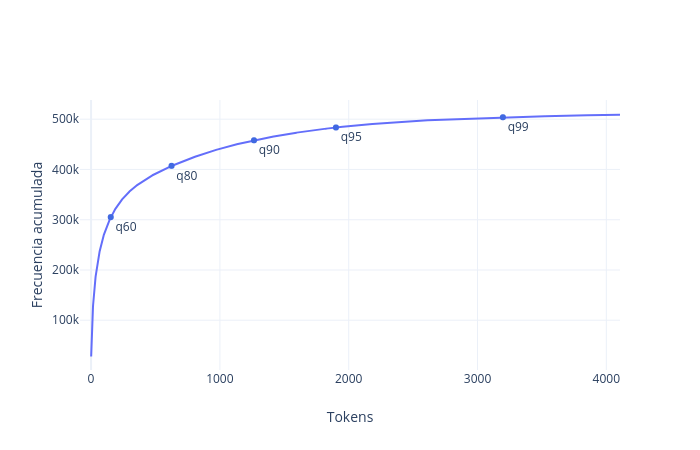
\includegraphics[width=0.8\textwidth]{experiments/cum_dist_2.png}
    \caption{Frecuencia acumulada de los tokens únicos aplicando hasta el cuarto nivel de procesamiento. El eje horizontal es el acumulado de tokens únicos en orden decreciente de ocurrencia. Los puntos corresponden a los cuantiles 60\%, 80\%, 90\%, 95\% y 99\%.}
    \label{img:cum_dist2}
\end{figure}

En la figura \ref{img:cum_dist2} se presenta la distribución acumulada del vocabulario hasta el cuarto nivel de procesamiento, en donde se observa que la cola de distribución es bastante menos pesada que bajo el primer nivel de procesamiento, además, como se observa en la tabla \ref{table:processing_stats} el tamaño del vocabulario se redujo a menos de un décimo del vocabulario obtenido bajo el primer nivel de procesamiento y es menos de un décimo del tamaño del corpus, por lo que bajo este nivel de procesamiento es posible desarrollar modelos con mayor fuerza estadística.

\begin{table}[H]
    \begin{tabular}{|c|r|r|r|}
        \hline
        procesamiento & \multicolumn{1}{c|}{documentos} & \multicolumn{1}{c|}{vocabulario} & \multicolumn{1}{c|}{tokens} \\ \hline
        raw          & 49.015                           & 79.327                            & 2.030.980                     \\ \hline
        ch    & 49.011                           & 46.708                            & 1.947.235                     \\ \hline
        ch+s+l+f      & 47.993                           & 4.106                             & 508.987                      \\ \hline
        \end{tabular}
    \caption{Estadísticas del corpus bajo distintos niveles de procesamientos, \textbf{raw}: sin procesamiento, \textbf{ch}: eliminación de símbolos de puntuación, correos electrónicos y tokens con números, \textbf{ch+s+l+f}: además incluye eliminación de stopwords (s), lemmatización (l) y eliminación de tokens con baja ocurrencia (f).}
    \label{table:processing_stats}
\end{table}


En la tabla \ref{table:innovation_rate} se muestra el detalle del vocabulario para cada una de las épocas tras procesar el corpus, de aquí se extrae que en promedio un 21.28\% del vocabulario se olvida de una época a otra y un 28.19\% es nuevo, es otras palabras, en promedio alrededor de un 50\% del vocabulario no es común entre tópicos de épocas adyacentes, esto justifica la necesidad de utilizar médidas de similitud que capturen la similitud entre palabras de épocas adyacentes ante la renovación que sufre el vocabulario en el tiempo.

\begin{table}[h]
    \begin{tabular}{|r|r|r|r|r|}
    \hline
    \textbf{época} & \textbf{old\_vocab} & \textbf{new\_vocab} & \textbf{\%old\_vocab} & \textbf{\%new\_vocab} \\ \hline
    2              & 1.919                     & 1.986                     & 23,35                 & 26.84                 \\ \hline
    3              & 1.986                     & 2.092                     & 22,61                 & 27.95                 \\ \hline 
    4              & 2.092                     & 2.414                     & 18,21                 & 33.60                 \\ \hline
    5              & 2.414                     & 2.629                     & 19,80                 & 28.71                 \\ \hline
    6              & 2.629                     & 2.666                     & 22,44                 & 23.85                 \\ \hline
    \end{tabular}
    \caption{Evolución del vocabulario en el tiempo, \textbf{old\_vocab}: corresponde al vocabulario del período $t-1$, \textbf{new\_vocab}: corresponde al vocabulario del período $t$, \textbf{\%old\_vocab}: porcentaje de tokens del período $t-1$ que ya no están en el período $t$ y \textbf{\%new\_vocab}: porcentaje de tokens del período $t$ que no están en el período $t-1$.}
    \label{table:innovation_rate}.
\end{table}

\section{Análisis cuantitativo de resultados}

Al aplicar HDP de forma independiente en cada una de los épocas se obtuvo el siguiente número de tópicos [8, 10, 9, 8, 8, 9].

\subsubsection{Distribución acumulada de los tópicos}
En la figura \ref{img:cum_dist3} se muestra la distribución acumulada promedio de los tópicos, se tiene que en promedio un 8.54\% y 21.42\% del vocabulario se puede capturar un 80\% y 95\% respectivamente de la distribución acumulada de los tópicos, además, para un 99\% de los tópicos basta con un 37\% del vocabulario para capturar el 95\% de su distribución acumulada, por tanto, una representación incompleta de los tópicos usando las palabras más probables que capturan el 80\% de la distribución acumulada trae consigo una disminución importante en el tamaño del vocabulario. 

% tabla con tiempos de ejecución

\begin{figure}
    \centering
    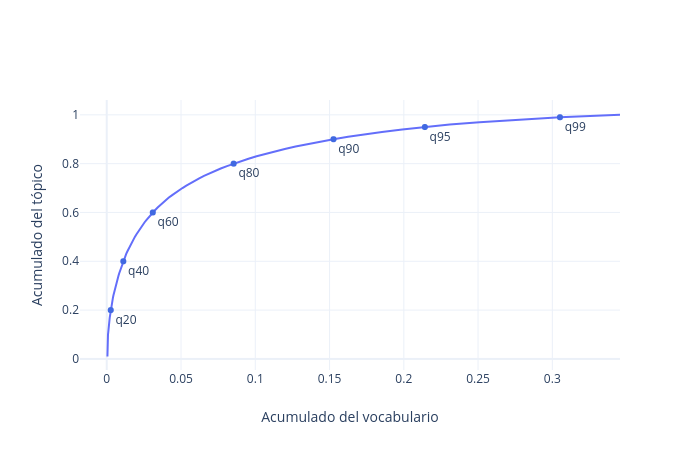
\includegraphics[width=0.8\textwidth]{experiments/cum_dist_3.png}
    \caption{Distribución acumulada promedio de los tópicos en función del vocabulario. El punto (x,y) en el gráfico corresponde a la fracción x del vocabulario que explica la fracción y de la distribución acumulada del tópico. Los puntos corresponden a los cuantiles 60\%, 80\%, 90\%, 95\% y 99\%.}
    \label{img:cum_dist3}
\end{figure}

\subsubsection{Construicción del grafo temporal}

El modelo propuesto considera tres hiperparámetros:
\begin{itemize}
    \item $q \in [0,1]$: para el cálculo de WMD se utilizan las palabras más probables del tópico que explican un 100q\% de la distribución acumulada del tópico. Este parámetro genera un nuevo tópico (se normaliza para sumar 1) con un vocabulario más reducido.
    \item $\lambda \in [0,1]$: este parámetro pondera la probabilidad de la palabra dentro del tópico con su exclusividad. El nuevo tópico generado es normalizado para sumar 1.
    \item $\zeta \in [0,1]$: punto operante de la cdf del grafo inicial, permite definir el cuantil que se usará como úmbral para eliminar arcos con similitud menor a este. 
\end{itemize}

Para entender de mejor manera la influencia de cada uno de estos parámetros se hizó un etiquetado de los arcos del grafo temporal, asignando un 1 a los arcos que deberían estar presente y 0 a los que no. Luego, se hizó una búsqueda a través de la siguiente grilla de parámetros, $\lambda \in \{0.2, 0.4, 0.6, 0.8, 1.0\}$, $q \in \{0.2, 0.4, 0.6, 0.8, 0.9, 0.95\}$ y $\zeta \in \{0.05, 0.10, ..., 0.90, 0.95\}$.\\

Como métrica de evaluación se propone \textit{F-score}, definida por:
\begin{align}
    F-score = 2\times \frac{\text{precision}\cdot \text{recall}}{\text{precision}+\text{recall}}
\end{align}
, donde \textit{recall} es la tasas de acierto sobre la clase positiva (presencia de un arco) y \textit{precision} es la tasa de acierto de las predicciones sobre la clase positiva. Esta métrica permite balancear la acertividad con la precisión, así una configuración que no pode ningún arco tendra un \textit{recall}=1, pero un bajo \textit{precision} (notar que el númerador decrece más rápido que el denominador). \\

De la figura \ref{img:f_score} se observa que \textit{F-score} tiende a ser creciente en función de $\zeta$, esto se debe a que menor $\zeta$ más falsos positivos (pues son más arcos los que sobreviven) empeorando así el \textit{precision} y por consecuencia el \textit{F-score}. Las configuraciones óptimas ocurren en su mayoría en $\zeta=0.95$ con excepción de tres configuraciones de las treinta posibles de $q\times \lambda$, las cuales se dan en $\zeta=0.9$ para los parámetros $q=0.2$ con $\lambda \in \{0.8, 1\}$ y $q=0.4$ con $\lambda=0.2$, sin embargo, el valor óptimo alcanzado es bastante cercano al obtenido con $\zeta=0.95$. En cuanto a $\lambda$ se observa que no existen muchas diferencias entre $\lambda\in\{0.6, 0.8, 1.0\}$ a diferencia de $\lambda \in \{0.2, 0.4\}$ que suele estar significativamente por debajo de las otras curvas, además se observa una dominancia débil en $\lambda$, es decir, en el $\zeta$ óptimo dado un $(q, \lambda)$ un $\lambda$ mayor no es peor. En el caso del parámetro $q$ se observa que para $q\geq 0.6$ el óptimo obtenido para $\lambda\geq 0.4$ es el mismo, en cambio para $q=0.4$ esto se cumple para todo $\lambda\geq 0.6$ y con $q=0.2$ para $\lambda \geq 0.8$. 

\begin{figure}
    \centering
    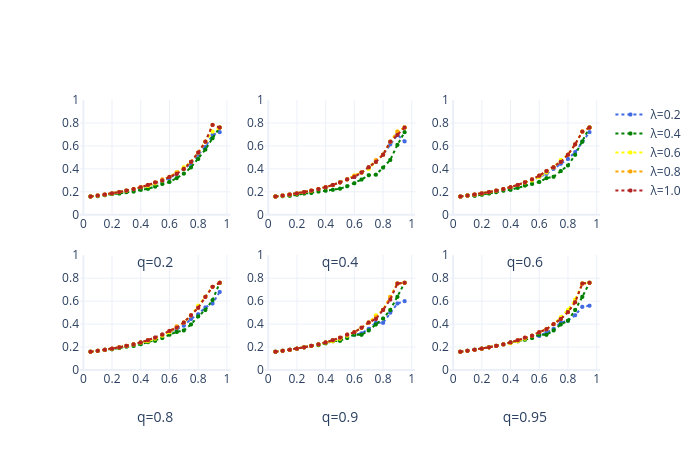
\includegraphics[width=1\textwidth]{experiments/f_score.png}
    \caption{F-score (eje vertical) para diferentes configuraciones de los hiperparámetros $q$, $\zeta$ (eje horizontal) y $\lambda$.}
    \label{img:f_score}
\end{figure}

De la tabla \ref{table:f_score} se observa que la configuración óptima se alcanza con $q=0.2$ con $\zeta=0.9$, además esto ocurre tanto para $\lambda=0.8$ como $\lambda=1.0$, por lo que es escoje la configuración $(q, \zeta, \lambda) = (0.2, 0.9, 1.0)$ para construir el grafo temporal. En la figura \ref{img:cdf} se observa la distribución acumulada de la similitud para el grafo completamente conectado, por lo que el para $zeta=0.9$ el úmbral viene siendo 0.21.

\begin{table}[H]
    \begin{tabular}{|c|c|c|c|c|}
    \hline
    \textbf{q} & \textbf{zeta} & \textbf{recall} & \textbf{precision} & \textbf{f-score} \\ \hline
    0.2        & 0.9           & 0.87            & 0.71               & 0.78             \\ \hline
    0.4        & 0.95          & 0.61            & 1                  & 0.76             \\ \hline
    0.6        & 0.95          & 0.61            & 1                  & 0.76             \\ \hline
    0.8        & 0.95          & 0.61            & 1                  & 0.76             \\ \hline
    0.9        & 0.95          & 0.61            & 1                  & 0.76             \\ \hline
    0.95       & 0.95          & 0.61            & 1                  & 0.76             \\ \hline
    \end{tabular}
    \caption{Configuración de $\zeta$ para cada $q$ que máximiza el \textit{F-score}.}
    \label{table:f_score}
\end{table}


\begin{figure}
    \centering
    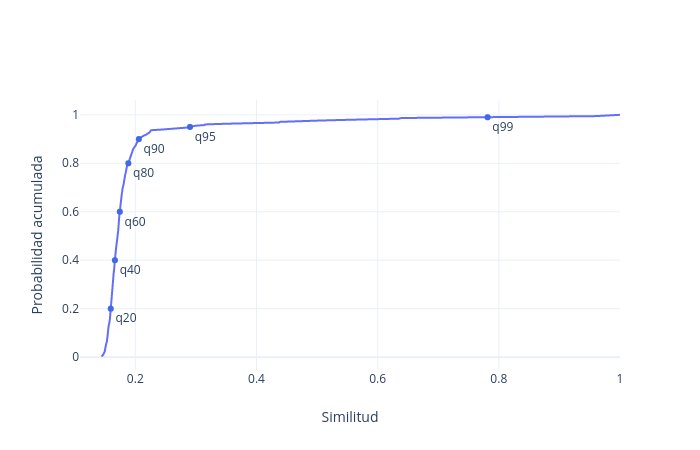
\includegraphics[width=0.8\textwidth]{experiments/cdf.png}
    \caption{Estimación empírica de la función de distribución acumulada (cdf) de la similitud entre tópicos correspondiente al grafo temporal completamente conectado para la configuración óptima $(q, \lambda)=(0.2, 1.0)$.}
    \label{img:cdf}
\end{figure}

% tratar de computar el caso donde q=1.0 (estimación de tiempo =100h)
En la figura \ref{img:speedup} se observa que la configuración óptima es en promedio 184 veces más eficiente que $q=0.95$, esto se debe a que $q=0.2$ es un 0.3\% del vocabulario (6 palabras en promedio) y $q=0.95$ alrededor de un 21\% (488 palabras en promedio).
\begin{figure}
    \centering
    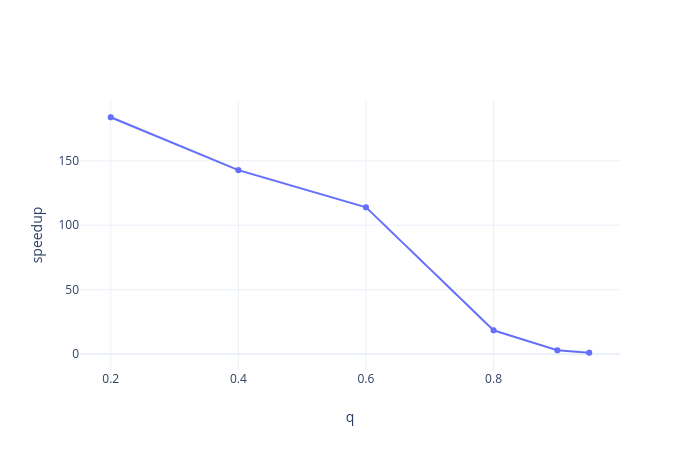
\includegraphics[width=1\textwidth]{experiments/speedup.png}
    \caption{Speedup promedio de la construcción del grafo en función de $q$. El speedup 1 equivale al tiempo más lento el cual está asciado a $q=0.95$ que es el valor de $q$ más grande y por ende con menor reducción de vocabulario de los tópicos a la hora de computar WMD.}
    \label{img:speedup}
\end{figure}

%\ref{img:ground_truth} y \ref{img:pruned_graph}
%conteo de arcos y blabla
%asociacion a tamaño de los topicos 
%no hablar todavía del significado de los tópicos

\begin{figure}
    \centering
    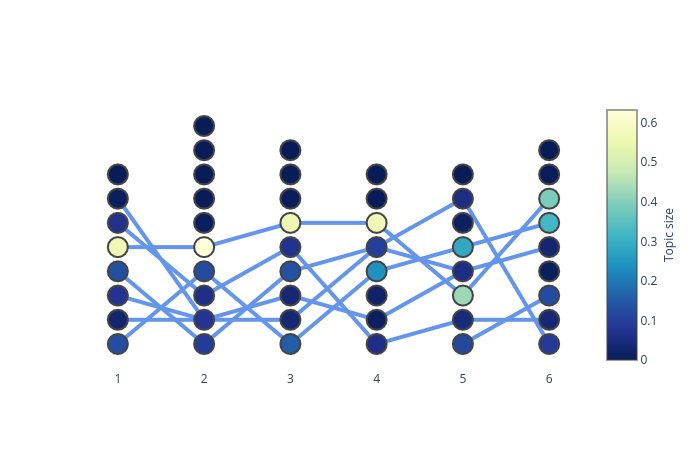
\includegraphics[width=0.8\textwidth]{experiments/ground_truth.png}
    \caption{Grafo temporal etiquetado.}
    \label{img:ground_truth}
\end{figure}

\begin{figure}
    \centering
    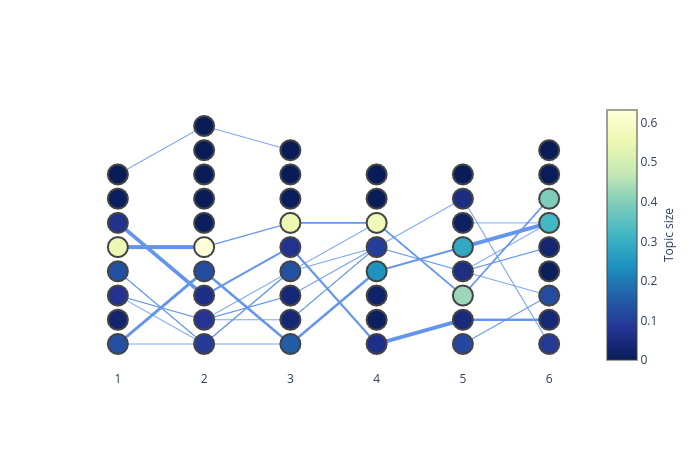
\includegraphics[width=0.8\textwidth]{experiments/pruned_graph.png}
    \caption{Grafo temporal obtenido a partir de la configuración óptima de parámetros $(q, \lambda, \zeta) = (0.2, 1.0, 0.9)$.}
    \label{img:pruned_graph}
\end{figure}
\section{Análisis cualitativo de resultados}


\chapter{Conclusiones}


\bibliography{main}

% FIN DEL DOCUMENTO
\end{document}
